\chapter{Search for new physics via top quark production in dilepton final state}\label{chap:tW}
\textit{This chapter introduced searching for new physics via top quark production in $ee$ and $\mu\mu$ final state. The data-set corresponds to an integrated luminosity of 35.9 \fbinv\ of proton-proton collisions at 13 TeV, and was collected in 2016 by the CMS detector. The search is sensitive to new physics in top quark pair production and in single top quark production in association with a W boson. This is the first search for new physics that uses the tW process.No significant deviation from the standard model expectation is observed.
Results are interpreted in the framework of an effective field theory and constraints on the relevant effective couplings are set using a dedicated multivariate analysis.}

\section{Introduction}
\label{tW_Int}



In this chapter, a search for new physics in top quark production using an EFT framework is reported. Final states with two same flavor opposite-sign isolated leptons (electrons or muons) in association with jets identified as originated from the fragmentation of a b quark (``b jets'') are analysed.
%The purpose of this paper is to search for new physics in tW and \ttbar production in dilepton final state using EFT framework.
The search is sensitive to new physics contributions to the tW and \ttbar ~production, and the six effective couplings, \CG, \Cphiq, \CtW, \CtG, \CuG, and \CcG, are constrained independently.
Kinematic distributions of final state particles and the production rate of the tW and \ttbar ~processes are both affected by the effective couplings. For the \Cphiq, \CtW, \CtG, and \CG effective couplings, the deviation from the SM prediction is dominated by the interference term between SM and new physics diagrams, which is linear with respect to the effective coupling. Therefore, kinematic distributions of final state particles vary as a function of Wilson coefficients and a small value of the effective couplings leads to distributions similar to the SM predictions.
On the other hand, the new physics terms for the \CuG and \CcG effective couplings do not interfere with the SM tW process, and the kinematic distributions of final state particles are determined by the new physics term independently of the SM prediction.
In this analysis, we use the rates of tW and \ttbar ~production for probing the \Cphiq, \CtW, \CtG, and \CG effective couplings, while both variation in rate and kinematic distributions of final state particles are employed  for probing the \CuG and \CcG effective couplings.





The chapter is structured as follows. In Section \ref{tW_Samples}, a description of the data and simulated samples used in the analysis is detailed. The trigger used in this analysis is detailed in Section \ref{tW_Trigger}. The object selection and event selection are presented in Section \ref{tW_Objectselection} and \ref{tW_Eventselection}, respectively. The SM background estimation and data mc distribution are presented in sections \ref{tW_background} and Section \ref{tW_data_mc}, respectively.
Section \ref{signal} presents a description of the signal extraction procedure.
An overview of the systematic uncertainty treatment is given in Section \ref{tW_systematic}. A cross check for measuring SM tW process cross section is provided in appendix \ref{App_tW_XS}.
Finally, the constraints on the effective couplings are presented in Section \ref{tW_Results}, and a summary is given in Section \ref{sec:tW_summary}.

\clearpage
\section{Data-sets and Monte Carlo Samples}
\label{tW_Samples}
\subsection{Data samples}
The primary data sets used in this analysis are summarised in Table \ref{data-samples}. The data from the
Moriond17 rereco campaign (Run2016 03Feb2017 Re-miniAOD) is used for eras 2016B through 2016G and the prompt reconstruction is used for era 2016H (Run2016H-03Feb2017\_ver2 and Run2016H-03Feb2017\_ver3).
The integrated luminosity of the data sample used in this analysis is $35.9$ fb$^{-1}$ collected by the CMS experiment in 2016.
Only certified data recommended for analysis by the PdmV group is used. The corresponding JSON file is the following:\\
Cert\_271036-284044\_13TeV\_23Sep2016ReReco\_Collisions16\_JSON.txt


\begin{table}[htp]
\small
\begin{center}
  \begin{tabular}{llc}
    \hline
    Datasets                &  run range & integrated luminosity (\pbinv)       \\  \hline \hline
    /X/Run2016B-03Feb2017\_ver2-v2/MINIAOD  & $273158 - 275376$ & $5788.348$ \\
    /X/Run2016C-03Feb2017-v1/MINIAOD  & $275657 - 276283$ & $2573.399$ \\
    /X/Run2016D-03Feb2017-v1/MINIAOD  & $276315 - 276811$ & $4248.384$ \\
    /X/Run2016E-03Feb2017-v1/MINIAOD  & $276831 - 277420$ & $4009.132$ \\
    /X/Run2016F-03Feb2017-v1/MINIAOD  & $277981 - 278808$ & $3101.618$ \\
    /X/Run2016G-03Feb2017-v1/MINIAOD  & $278820 - 280385$ & $7540.488$ \\
    /X/Run2016H-03Feb2017\_ver2-v1/MINIAOD & $281613 - 284035$ & $8390.540$ \\
    /X/Run2016H-03Feb2017\_ver3-v1/MINIAOD & $284036 - 284044$ & $215.149$ \\ \hline
    Sum & $273158 - 284044$ & $35.867$ \\ \hline
  \end{tabular}
\end{center}
\caption{Data sets (X) used in this analysis. X = 'DoubleEG' and 'SingleElectron' for the $ee$ channel. X = 'DoubleMuon' and 'SingleMuon' for $\mu\mu$ channel analysis.}
%\caption{Data sets (X) used in this analysis. X = 'DoubleEG' and 'SingleElectron' for the $ee$ channel. X = 'MuonEG','SingleElectron' and 'SingleMuon' for $e\mu$ channel. X = 'DoubleMuon' and 'SingleMuon' for $\mu\mu$ channel analysis. X = 'MET' for trigger efficiency and scale factor study. The run ranges are adjusted to only include good runs.}
\label{data-samples}
\end{table}

\subsection{MC samples}
The analysis uses centrally produced Monte Carlo (MC) samples from  'RunIISummer16 MiniAODv2' campaign as are recommended for  Moriond17.
For the MC samples used, GEN-SIM was produced using CMSSW\_7\_1\_X and the DIGI-RECO was produced using CMSSW\_8\_0\_X.
All the MC are listed in Table \ref{mc-samples}.



\begin{table}[h]

\centering
\small
\smallskip\noindent
\resizebox{\linewidth}{!}{%
\begin{tabular}{llll}
\hline
sample                                                                     & xsection(pb)  & xs precision  \\
\hline
\hline
DYJetsToLL\_M-10to50\_TuneCUETP8M1\_13TeV-amcatnloFXFX-pythia8             & 18610         & NLO             \\
DYJetsToLL\_M-50\_TuneCUETP8M1\_13TeV-amcatnloFXFX-pythia8                 & 5765.4        & NNLO            \\
\hline
WWTo2L2Nu\_13TeV-powheg                                                    & 12.178        & NNLO             \\
WZTo3LNu\_TuneCUETP8M1\_13TeV-powheg-pythia8                               & 4.42965       & NLO              \\
WZTo2L2Q\_13TeV\_amcatnloFXFX\_madspin\_pythia8                            & 5.595         & NLO              \\
ZZTo2L2Nu\_13TeV\_powheg\_pythia8                                          & 0.564         & NLO              \\
ZZTo4L\_13TeV\_powheg\_pythia8                                             & 1.212         & NLO              \\
WGToLNuG\_TuneCUETP8M1\_13TeV-amcatnloFXFX-pythia8                         & 489           & NLO              \\
\hline
ST\_tW\_top\_5f\_NoFullyHadronicDecays\_13TeV-powheg\_TuneCUETP8M1         & 19.47         & app.NNLO         \\
ST\_tW\_antitop\_5f\_NoFullyHadronicDecays\_13TeV-powheg\_TuneCUETP8M1     & 19.47         & app.NNLO         \\
TTTo2L2Nu\_TuneCUETP8M2\_ttHtranche3\_13TeV-powheg                         & 87.31         & NNLO             \\
TTWJetsToQQ\_TuneCUETP8M1\_13TeV-amcatnloFXFX-madspin-pythia8              & 0.4062        & NLO             \\
TTWJetsToLNu\_TuneCUETP8M1\_13TeV-amcatnloFXFX-madspin-pythia8             & 0.2043        & NLO             \\
TTZToLLNuNu\_M-10\_TuneCUETP8M1\_13TeV-amcatnlo-pythia8                    & 0.2529        & NLO             \\
TTZToQQ\_TuneCUETP8M1\_13TeV-amcatnlo-pythia8                              & 0.5297        & NLO             \\
TTGJets\_TuneCUETP8M1\_13TeV-amcatnloFXFX-madspin-pythia8                  & 3.697         & NLO             \\
\hline
WJetsToLNu\_TuneCUETP8M1\_13TeV-madgraphMLM-pythia8                        & 61526.7       & NNLO            \\
\hline
GluGluHToWWTo2L2Nu\_M125\_13TeV\_powheg\_pythia8                           & 2.5           & NLO             \\
VBFHToWWTo2L2Nu\_M125\_13TeV\_powheg\_pythia8                              & 0.175         & NLO             \\
\hline
\hline
\end{tabular}}
\caption{MC samples \tiny{(dataset=/*/RunIISummer16MiniAODv2*PUMoriond17\_80X\_mcRun2\_asymptotic\_2016\_TrancheIV\_v6*/MINIAODSIM)}}
\label{mc-samples}
\end{table}

The pile up distributions for MC and data which is calculated by using 69.2 mb as the minimum bias cross section are shown in left of Figure \ref{fig:Z_pileup}. MC events are re-weighted to account for the pile up difference between data and MC.

%In the 5 flavor scheme,
%the tW single top-quark process overlaps and interferes with \ttbar production
%at NLO where diagrams involving two top quarks are part of the real emission corrections to
%tW production~\cite{Campbell:2005bb,Frixione:2005vw}.
%A calculation in the 4 flavor scheme
%includes tW and \ttbar as well as non-top-quark diagrams~\cite{Cascioli:2013wga} and
%the interference between tW and \ttbar enters already at tree level.
%The diagram removal (DR) scheme \cite{Frixione:2008yi}, in which all next-to-leading order (NLO)
%diagrams that overlap with the \ttbar definition are removed from the calculation of the tW
%amplitude, was employed to handle interference between tW
%and \ttbar diagrams, and was applied to the tW sample.
%
%The DR scheme was employed to handle interference between tW and \ttbar diagrams, and was applied to the tW sample.

%For plotting and comparing pre-fit MC predictions to data, the predicted tW cross-section at a $\sqrt{s}=13$ TeV is set to the NLO value with next-to-next-to-leading logarithmic (NNLL) soft-gluon corrections, calculated as
%$\sigma_{\text{theory}}=71.7\pm1.8\,(scale)\pm{3.4}\,(PDF)$ ~\cite{Kidonakis:2015},
%assuming a top quark mass ($m_{\text{top}}$) of 172.5 GeV.
%The first uncertainty accounts for the renormalisation and factorisation scale variations (from $m_{\text{top}}/2$ to $2 \,m_{\text{top}}$), while the second uncertainty originates from uncertainties in the MSTW2008 NLO parton distribution function (PDF) sets.


\section{Triggers}
\label{tW_Trigger}

In this analysis we use various sets of triggers in order to achieve an optimal selection efficiency.
For each dilepton channel (ee, $\mu\mu$) we take the logical OR of the dilepton triggers listed
in Table \ref{tab:trigger}.
The increase of the instantaneous luminosity delivered by the LHC in Run H needed the (re)introduction of the DZ cut for pure dimuon trigger.

We complement the partially inefficient dilepton triggers by single lepton triggers and remove the overlap between two
primary data sets by vetoing events that fired a dilepton trigger in the single lepton primary
data sets.
%Because the e$\mu$ channel is complemented by two single lepton primary data sets, the
%procedure has two steps: We first add events from the SingleElectron primary data set that
%fired single electron triggers but failed the double lepton triggers that we use to select events
%in the MuonEG primary data set. We furthermore add events from the SingleMuon primary
%data set that fired single muon triggers but fired none of the triggers we use to select events in
%either the MuonEG or the SingleElectron primary data set.
Table \ref{tab:trigger} gives an overview of all triggers used in this analysis.
Using \ttbar ~and tW MC samples, it is found that by adding single lepton triggers, trigger efficiency is increased by around 5\%.


% Please add the following required packages to your document preamble:
%\usepackage{multirow}
\begin{table}[th]
\centering
\begin{tabular}{lll}
\hline
channel               & path                                                      & dataset             \\ \hline \hline
\multirow{2}{*}{ee}   & HLT\_Ele23\_Ele12\_caloIdL\_TrackIdL\_IsoVL\_DZ           & data \& MC          \\
                      & HLT\_Ele27\_WPTight\_Gsf                                  & data \& MC          \\ \hline
%\multirow{7}{*}{e$\mu$}  & HLT\_Mu8\_TrkIsoVVL\_Ele23\_CaloIdL\_TrackIdL\_IsoVL      & data runs B-G \& MC \\
%                      & HLT\_Mu23\_TrkIsoVVL\_Ele12\_CaloIdL\_TrackIdL\_IsoVL     & data runs B-G \& MC \\
%                      & HLT\_Mu8\_TrkIsoVVL\_Ele23\_CaloIdL\_TrackIdL\_IsoVL\_DZ  & data only run H \\
%                      & HLT\_Mu23\_TrkIsoVVL\_Ele12\_CaloIdL\_TrackIdL\_IsoVL\_DZ & data only run H \\
%                      & HLT\_Ele27\_WPTight\_Gsf                                  & data \& MC          \\
%                      & HLT\_IsoMu24                                              & data \& MC          \\
%                      & HLT\_IsoTkMu24                                            & data \& MC          \\ \hline
\multirow{6}{*}{$\mu\mu$} & HLT\_Mu17\_TrkIsoVVL\_Mu8\_TrkIsoVVL                      & data runs B-G \& MC \\
                      & HLT\_Mu17\_TrkIsoVVL\_TkMu8\_TrkIsoVVL                    & data runs B-G \& MC \\
                      & HLT\_Mu17\_TrkIsoVVL\_Mu8\_TrkIsoVVL\_DZ                  & data only run H     \\
                      & HLT\_Mu17\_TrkIsoVVL\_TkMu8\_TrkIsoVVL\_DZ                & data only run H     \\
                      & HLT\_IsoMu24                                              & data \& MC          \\
                      & HLT\_IsoTkMu24                                            & data \& MC          \\ \hline \hline
\end{tabular}
\caption{Summary of the signal triggers}
\label{tab:trigger}
\end{table}


Since the trigger information is available in simulated samples, we require FullSim MC samples to fire the trigger and finally apply corrections for any data/MC disagreement using scale factors.
TOP group recommended trigger scale factor (described in \cite{trSF}) are used.
We also have found trigger scale factors as a cross checked which gives similar result (although they are not used in this analysis).

\clearpage
\section{Object Identification}
\label{tW_Objectselection}
The tW  process in dilepton final states is characterised by the presence of two high \pt leptons associated with missing transverse energy and one b-jet. The identifications for different object are presented in the following.

\subsection{Lepton selection}
\subsubsection{Muon}

The muons used in this analysis  are selected inside the fiducial region of the muon
spectrometer, $\abs{\eta}<  2.4$, with a minimum \pt  of 20 GeV, and using standard identification criteria, suggested by the Muon Physics Object Group (POG). Furthermore, they are required to be particle-flow (see Section \ref{sec:PF_algorithm}) muons.
Cuts are applied on the quality of the track fit, number of hits in the pixel, tracker and number
of matched muon segments for the muons to be considered for the dilepton candidate. These
requirements are summarized in the following and correspond to the so-called Tight muon identification \cite{muonid}.

$\bullet$ $\pt>$ 20 GeV and $\abs{\eta}<  2.4$,

$\bullet$ is a GlobalMuon and PFMuon,

$\bullet$ number of matched Stations $> $1,

$\bullet$ number of pixel hits $>$ 0,

$\bullet$ number of hits in the inner tracker $>$ 5,

$\bullet$ number of muon hits $>$ 0,

$\bullet$ $\frac{\chi^2}{NDF}$ of the global-muon track fit $<$ 10,

$\bullet$ Impact parameter constrains between the muon track and the selected primary vertex dZ $<$ 0.5  and d0 $<$ 0.2 cm.


For the muon isolation, a cone of $\Delta R = 0.4$ is built to
compute the flux of particle flow candidates, the $\Delta\beta$ correction is applied to correct
for pileup (PU) contamination. This correction is achieved by subtracting half the sum of the \pt of
the charged particles in the cone of interest but with particles not originating from the primary
vertex (PV).
The muon isolation is therefore defined as:
\begin{eqnarray}
\label{eq:Irel}
I_{rel}^{\mu} = \frac{1}{\pt^{\mu}} &(&\Sigma \pt(\text{ch-had from PV}) + max(0,\Sigma \et(\text{neut-had}) \nonumber \\
&+&  \Sigma \et(\text{photon}) - 0.5 \Sigma \pt(\text{ch-had from PU}))),
\end{eqnarray}
where ``ch-had'' means charged hadron and ``neut-had'' means neutral hadron.
The factor $0.5$ corresponds to an approximate average of neutral to charged particles and has
been measured in jets in Ref. \cite{CMS:2010eua}. In our analysis the muon candidates must have $I_{rel}^{\mu}<0.15$ to be
considered as isolated \cite{muonid}.
Scale factors are used to correct for differences in the reconstruction, ID and Isolation efficiencies in data and MC. They are evaluated using the tag and probe technique, and both
the scale factors and their uncertainty prescriptions are provided by the Muon POG \cite{muonsf}.
In addition, muon energy scale and smearing is applied  based on Rochester group  recommendations \cite{Rochester}.


\subsubsection{Electron}

Electron candidates are selected from the reconstructed gsf electrons with  $ \pt>$ 20 GeV and $\abs{\eta}<$ 2.4 while the ECAL barrel-endcap gap is removed ($1.4442 < \abs{\eta_{SC}}< 1.566$, the $\eta_{SC}$ is the $\eta$ of super-cluster (see Section \ref{subsec:super-cluster}) corresponding to the electron).
Electrons need to pass the tight cut based POG recommended working point \cite{eleid} which includes the requirement to pass the conversion veto.
The Table \ref{Tab.electrontightidentification} contains the cuts used for the tight electron identification and more details can be found in \cite{eleid}.
%\cite{https://twiki.cern.ch/twiki/bin/viewauth/CMS/CutBasedElectronIdentificationRun2},
%Additionally, we apply cuts on the longitudinal and transverse impact parameter with respect to the primary vertex, which are removed from the official working point variable list. It is shown by TOP Physics Analysis Group (PAG) that electron ID scale factors are not changed by adding these two extra variables with respect to official tight working point \cite{eleid}.

\begin{table}[!h]
\begin{center}
\begin{tabular}{lll}
\hline\hline
                & Barrel$(\abs{\eta_{SC} })<=1.479 $& Endcap$(\abs{\eta_{SC} })>1.479 $  \\
\hline
full5$\times$5 $\sigma_{\mathrm{I}_{\eta} \mathrm{I}_{\eta}} < $ & $0.00998$ & $0.0292$ \\
$\abs {\Delta\eta_{\mathrm{Inseed}}}<$ & $0.00308$ & $0.00605$ \\
$\abs{\Delta \Phi_{\mathrm{In}}}<$ &$0.0816$ &$0.0394$ \\
H/E $<$& $0.0414$ & $0.0641$ \\
relative electron isolation $<$& $0.0588$&$0.0571$\\
$\abs{\mathrm{(1/E-1/P)}}<$ &0.0129&0.0129\\
expected missing inner hits$<=$&1 &1\\
pass conversion veto & yes& yes \\
d0 $<$&  $0.05$ & $0.1$ \\
dZ $<$&  $0.1 $ & $0.2$ \\
\hline
\end{tabular}
\caption{  The cuts for the electron identification in the barrel and endcap.}
\label{Tab.electrontightidentification}
\end{center}
\end{table}


An Multivariate Analysis (MVA) regression technique is used to find the corrections for the super-cluster energy to account for the effects like energy leakage into the gaps between crystals, energy leakage into the HCAL downstream the ECAL, etc \cite{Khachatryan:2015hwa}. In addition, electron energy scale and smearing is applied  based on Egamma POG recommendations \cite{elescale}.
%The regression which is used in RunIISummer16 MiniAODv2 MC samples is trained using CMSSW74X.
%EGamma POG has provided 80 regression which should be applied offline to find the correct electron energy. 80 electron regression is applied as is explained in \cite{elereg}.



\subsection{Jet selection}

Particle candidates found by the PF algorithm are clustered into jets using the anti-$\mathrm{k_T}$ algorithm (see Section \ref{sec:Jets})
 with distance parameter R =0.4. The influence of pileup is mitigated by the Charged
Hadron Subtraction (CHS) technique which removes tracks identified as originating from pileup vertices. Jets are calibrated
in simulation and in data separately, accounting for deposits from pile-up and the imperfect detector response.
Level 1 corrections (which removes the energy coming from pile-up events), Level 2 and Level 3 MC-truth jet energy corrections as well as Level 2 and Level 3 residual corrections (which corrects the remaining small differences for jet response in data and MC, it is applied only for data) are applied using the latest set of Jet Energy Corrections (JECs).
Jets in MC are smeared using the latest set of Jet Energy Resolutions (JERs).
Corrected jets with $\pt >$ 30 GeV and $\abs{\eta} <2.4$ are selected if they pass the
loose jet identification criteria \cite{jetid}, i.e. the neutral electromagnetic and hadron fractions are
 $<$ 99\% and the jet consists of at least two PF candidates. Furthermore, both the charged hadron
fraction and multiplicity are required to be $>$ 0 and the charged electromagnetic fraction has to be $<$ 99\%.

Selected jet may still overlap with the selected leptons. This is possible because the lepton
can be clustered into a jet as well. To prevent such cases, jets that are found within a cone of
R = 0.4 around any of the selected signal leptons are removed from the set of selected jets.

Jets originating from the hadronization of b-quarks are identified using the Combined Secondary Vertex version 2 algorithm (CSVv2). The CSVv2 is based on secondary vertex and track-based lifetime information, it is an updated version of the CSV algorithm (see Section \ref{subsec:b-jet}) by combining the variables with a neural network instead of a likelihood ratio. In this analysis, a jet is b-tagged when its CSVv2 value passes the medium working point (i.e. CSVv2 $>$ 0.8484) \cite{bjet}.


\subsection{Missing Transverse Energy}

Missing transverse energy (MET, see the definition in Section \ref{sec:MET}) is calculated as the negative of the vectorial sum of the transverse
momentum vectors of all PF candidates in an event. To make MET a better estimate of true
invisible particles, so called Type-1 plus smeared corrections are applied, which propagate the jet energy
corrections to the raw MET \cite{metcor}.
%Latest T$_{xy}$-Shift correction is also provided and compared with T1 only corrections.
%Due to corrections related to muons and high energy electrons in reMiniAOD campain, 'slimmedMETsMuEGClean' collection is used.


In order to reduce the instrumental noise in the detector, MET filters are applied as are recommended by Jet-MET POG \cite{metfilter}.
These filters are summarized below:

$\bullet$ HBHENoiseFilter (data and MC),

$\bullet$ HBHENoiseIsoFilter (data and MC),

$\bullet$ globalTightHalo2016Filter (data and MC),

$\bullet$ goodVertices (data and MC),

$\bullet$ EcalDeadCellTriggerPrimitiveFilter (data and MC),

$\bullet$ BadChargedCandidateFilter (data and MC),

$\bullet$ BadPFMuonFilter (data and MC),

$\bullet$ eeBadScFilter (only data)

\subsection{Scale factors}

In the following, object related scale factors used in this analysis are listed:
\medskip

Muon: {\small\url{https://twiki.cern.ch/twiki/bin/view/CMS/MuonWorkInProgressAndPagResults#Results\_on\_the\_full\_2016\_data}}

$\bullet$ Tracking efficiency
{\small\url{https://test-calderona.web.cern.ch/test-calderona/MuonPOG/2016dataReRecoEfficiencies/tracking/Tracking\_EfficienciesAndSF\_BCDEFGH.root}}

$\bullet$ Identification efficiency
{\small\url{https://gaperrin.web.cern.ch/gaperrin/tnp/TnP2016/2016Data\_Moriond2017\_6\_12\_16/JSON/RunBCDEF/EfficienciesAndSF\_BCDEF.root}},
{\small\url{https://gaperrin.web.cern.ch/gaperrin/tnp/TnP2016/2016Data Moriond2017\_6\_12\_16/JSON/RunGH/EfficienciesAndSF\_GH.root}}

$\bullet$ Isolation efficiency
{\small\url{https://test-calderona.web.cern.ch/test-calderona/MuonPOG/2016dataReRecoEfficiencies/isolation/EfficienciesAndSF\_BCDEF.root}},
{\small\url{https://test-calderona.web.cern.ch/test-calderona/MuonPOG/2016dataReRecoEfficiencies/isolation/EfficienciesAndSF\_GH.root}}
\medskip

Electron: {\small\url{https://twiki.cern.ch/twiki/bin/view/CMS/EgammaIDRecipesRun2#Efficiencies\_and\_scale\_factors}}

$\bullet$ Reconstruction efficiency
{\small\url{http://fcouderc.web.cern.ch/fcouderc/EGamma/scaleFactors/Moriond17/approval/RECO/passingRECO/egammaEffi.txt\_EGM2D.root}}

$\bullet$ Identification + isolation efficiency
{\small\url{http://fcouderc.web.cern.ch/fcouderc/EGamma/scaleFactors/Moriond17/approval/EleID/passingTight80X/egammaEffi.txt\_EGM2D.root}}
\medskip

B-tagging: {\small\url{https://twiki.cern.ch/twiki/bin/viewauth/CMS/BtagRecommendation80XReReco}}

$\bullet$ b-tagging efficiency

\subsection{Top \pt reweighting}
In order to better describe the \pt distribution of the top quark in \ttbar events, the top quark \pt spectrum simulated with {\sc Powheg} is reweighted to match the differential top quark \pt distribution at NNLO QCD accuracy and includes EW corrections calculated in Ref. \cite{Czakon:2017wor}.

\clearpage
\section{Event Selection}
\label{tW_Eventselection}
The selection of the events to be used for our search is done in two steps which are explained in the following sections.
\subsection{Event selection (step 1)}
\label{step1_selection}
At the first step, we focus on selecting events by requiring trigger and lepton selection. Events should fire one of the triggers summarized in Table \ref{tab:trigger}.
At least 1 pair of opposite charge leptons with invariant mass $>$ 20 GeV is required while the leading lepton should have \pt $>$ 25 GeV.
The first two selected leptons which are sorted due to the \pt should have the same flavor and opposite sign. If the two highest \pt leptons have different flavors (e.g. e$\mu$ event) or same sign, the event is rejected.
The events are divided in the ee and \mumu channels according to the flavours of the two leptons with the highest \pt
and are further categorised in different bins depending on the number of jets (``n-jets'') in the final state and the number of them which are b-tagged (``m-tags'').
The largest number of  tW events is expected in the category with exactly one  b-tagged jet (1-jet,1-tag) followed by the category with two jets, one of which being a  b jet (2-jets,1-tag). Events in the categories with more than  two jets and exactly two b-tagged jets  are dominated by $\ttbar$ process ($\geq$2-jets,2-tags).

%Some distributions for Data/MC comparison after this step are shown in figures \ref{fig:step1_leading_lepton1}-\ref{fig:step1_Nvtx_jet_bjet}.
%In Figure \ref{fig:step1_MET_phi}, one can see that the  Data/MC agreement for MET distribution in ee and \mumu channels are not good. We have investigated this problem (see Appendix \ref{MET_disagreement_investigation}).
%
%
%Number of events for data and SM prediction using MC simulation after step 1 selection are summarized in Table \ref{tab:cut_flow_step1}.

\subsection{Event selection (step 2)}
\label{step2_selection}
%\subsubsection{Same flavour channels}
%No further cut applied for $e\mu$ channel.
In order to suppress the contribution of Drell-Yan events, we reject events with a dilepton invariant mass around the Z peak [76, 106]. In addition, a MET cut $>60$ GeV is applied. In Figure \ref{fig:step1_MET_phi}, one can see that the  Data/MC agreements for MET distributions in ee and \mumu channels are not good. We have investigated this problem (see Appendix \ref{MET_disagreement_investigation}). Because of that the normalization of the DY background simulation is estimated from data which is described in Section \ref{tW_DY_background}.
The final event selection criteria are shown in Table \ref{tab:Event-selection}.
\begin{table}[h]
\centering
\begin{tabular}{|l|l|c|}
\hline
\multirow{3}{*}{Step 1}         &                                                                                         & ee and \mumu           \\ \cline{2-3}
                                & $\pt^{\text{leading lepton}}>$ 25 GeV and $\pt^{\text{sub-leading lepton}}>$ 20 GeV & $\surd$                     \\ \cline{2-3}
                                & Mass(ll)$>$ 20 GeV                                                                      & $\surd$                     \\ \cline{2-3}
                                & The two highest \pt leptons should have same flavor and opposite charge             & $\surd$                     \\ \hline
\multirow{2}{*}{Step 2}         & MET $>$ 60 GeV                                                                          & $\surd$                     \\ \cline{2-3}
                                & Mass(ll) $<76$ or $>106$ GeV                                                            & $\surd$                     \\ \hline
\end{tabular}
\caption{Event selection criteria for ee and \mumu channels}
\label{tab:Event-selection}
\end{table}

\begin{figure}[ht]
  \begin{center}
    \begin{tabular}{ccc}
      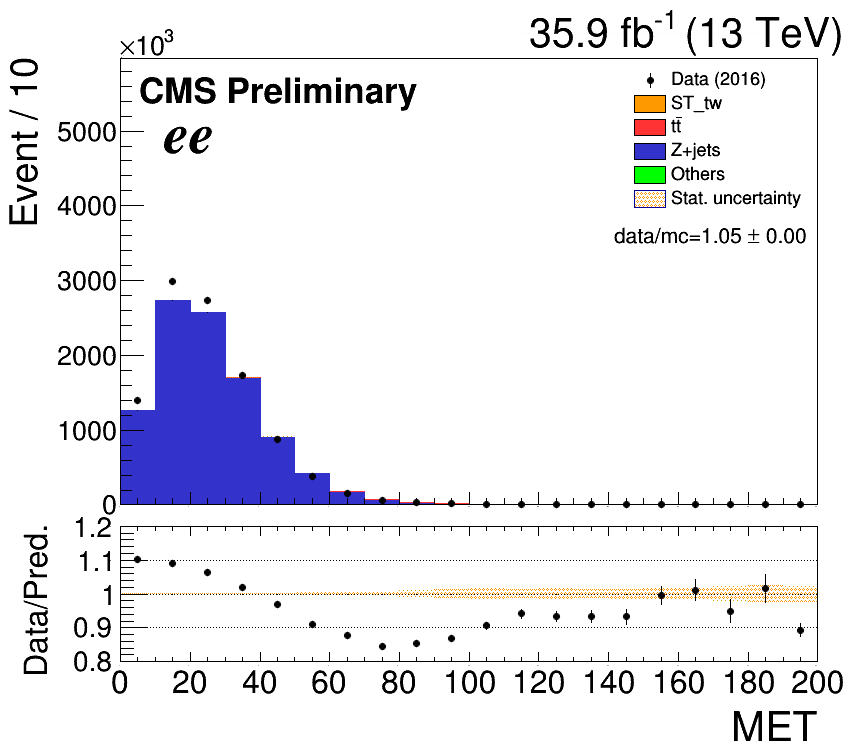
\includegraphics[width=0.49\textwidth]{figures/tW/fig/Step1/ee_noNvtx/H_MET_Et.png}&
      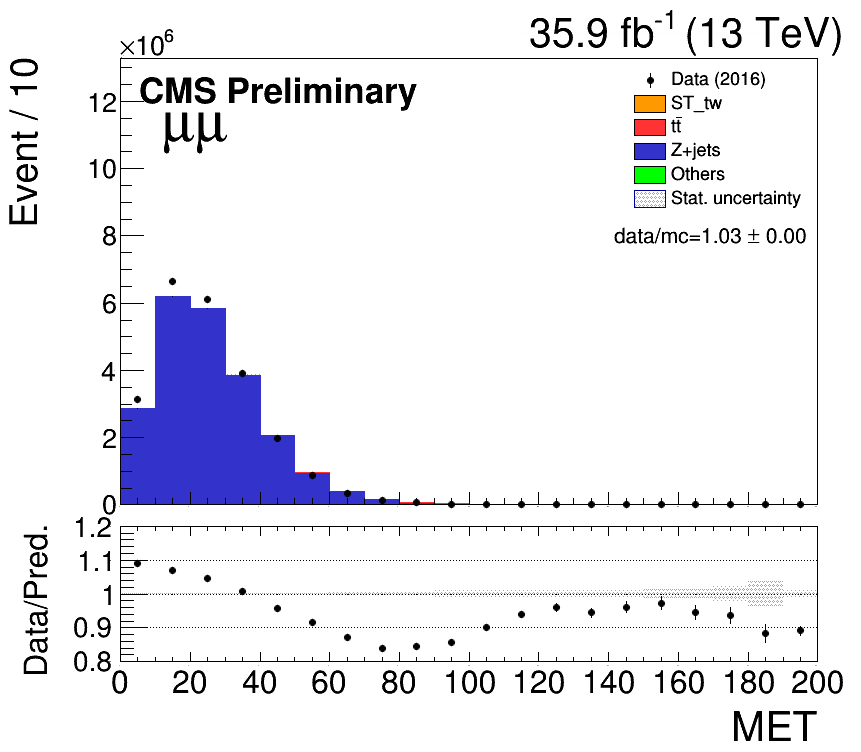
\includegraphics[width=0.49\textwidth]{figures/tW/fig/Step1/mumu_noNvtx/H_MET_Et.png}\\
    \end{tabular}
    \caption{The distributions of MET for ee (left) and \mumu (right) channels after step 1 selection. All backgrounds are estimated from MC simulations.}
    \label{fig:step1_MET_phi}
  \end{center}
\end{figure}

%\begin{table}[h]
%\centering
%\begin{tabular}{|l|l|c|c|}
%\hline
%\multirow{3}{*}{Step 1}         &                                                       & ee and \mumu     & $e\mu$        \\ \cline{2-4}
%                                & $\pt^{\text{leading lepton}}>$ 25 GeV and $\pt^{\text{sub-leading lepton}}>$ 20 GeV & $\surd$               & $\surd$       \\ \cline{2-4}
%                                & Mass(ll)$>$ 20 GeV                                    & $\surd$               & $\surd$       \\ \cline{2-4}
%                                & The two highest \pt leptons should have opoosite charge       & $\surd$               & $\surd$       \\ \hline
%\multirow{2}{*}{Step 2}         & MET $>$ 60 GeV                                        & $\surd$               & -       \\ \cline{2-4}
%                                & Mass(ll) $<76$ or $>106$ GeV                          & $\surd$               & -            \\ \hline
%\end{tabular}
%\caption{Event Selections}
%\label{tab:Event-selection}
%\end{table}

%\begin{table}[ht]
%\centering
%\begin{tabular}{|c|c|c||c|c|}
%\hline
%Channel & ee                   & fraction & \mumu            &fraction \\ \hline
%tW      & 8242      +/- 26       & 0.08\%   & 16259     +/- 37    & 0.07\%  \\ \hline
%TTbar   & 82120     +/- 62       & 0.83\%   & 165203    +/- 90    & 0.73\%  \\ \hline
%DY      & 9822251   +/- 6708     & 98.82\%  & 22325807  +/- 10376 & 98.96\% \\ \hline
%WW      & 8774      +/- 47       & 0.09\%   & 18933     +/- 71    & 0.08\%  \\ \hline
%WG      & 1280      +/- 75       & 0.01\%   & 334       +/- 38    & 0.00\%  \\ \hline
%Wjets   & 2173      +/- 296      & 0.02\%   & 1910      +/- 283   & 0.01\%  \\ \hline
%WZ      & 11056     +/- 23       & 0.11\%   & 22753     +/- 33    & 0.10\%  \\ \hline
%TTG     & 434       +/- 10       & 0.00\%   & 761       +/- 13    & 0.00\%  \\ \hline
%ZZ      & 2712      +/- 3        & 0.03\%   & 5880      +/- 5     & 0.03\%  \\ \hline
%HWW     & 782       +/- 11       & 0.01\%   & 1885      +/- 18    & 0.01\%  \\ \hline
%TTWJets & 38        +/- 4        & 0.00\%   & 72        +/- 5     & 0.00\%  \\ \hline \hline
%data    & 10406970  +/- 3226     &          & 23278344  +/- 4825  &         \\ \hline
%Pred    & 9939863   +/- 6715     &          & 22559798  +/- 10381 &         \\ \hline
%
%\hline
%\hline
%Channel & $e\mu$          & fraction   & $Combined$          &fraction \\ \hline
%tW      & 23057   +/- 43  & 6.43\%     & 47558     +/- 62    & 0.14\%  \\ \hline
%TTbar   & 232161  +/- 106 & 64.76\%    & 479484    +/- 153   & 1.46\%  \\ \hline
%DY      & 64880   +/- 559 & 18.10\%    & 32212938  +/- 12368 & 98.04\% \\ \hline
%WW      & 25864   +/- 82  & 7.21\%     & 53571     +/- 118   & 0.16\%  \\ \hline
%WG      & 1958    +/- 95  & 0.55\%     & 3572      +/- 127   & 0.01\%  \\ \hline
%Wjets   & 4060    +/- 412 & 1.13\%     & 8142      +/- 581   & 0.02\%  \\ \hline
%WZ      & 2369    +/- 14  & 0.66\%     & 36179     +/- 43    & 0.11\%  \\ \hline
%TTG     & 1115    +/- 16  & 0.31\%     & 2310      +/- 23    & 0.01\%  \\ \hline
%ZZ      & 484     +/- 2   & 0.13\%     & 9076      +/- 7     & 0.03\%  \\ \hline
%HWW     & 2430    +/- 20  & 0.68\%     & 5097      +/- 29    & 0.02\%  \\ \hline
%TTWJets & 121     +/- 7   & 0.03\%     & 231       +/- 9     & 0.00\%  \\ \hline \hline
%data    & 356383  +/- 597 &            & 34041697  +/- 5835  &         \\ \hline
%Pred    & 358497  +/- 716 &            & 32858157  +/- 12384 &         \\ \hline
%
%\end{tabular}
%\caption{Cut flow Table after step1 (trigger and lepton selections). Number of background events  are estimated using MC simulated samples and  errors are MC statistical uncertainties only. }
%\label{tab:cut_flow_step1}
%\end{table}
%
%\begin{figure}[ht]
%  \begin{center}
%    \begin{tabular}{ccc}
%      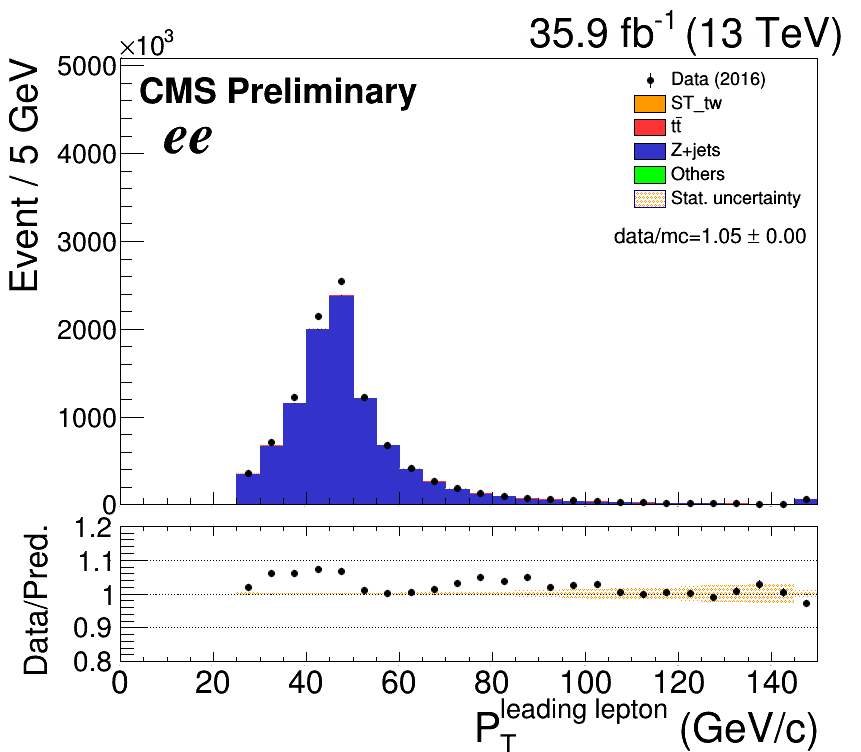
\includegraphics[width=0.32\textwidth]{figures/tW/fig/Step1/ee_noNvtx/H_lepton_led_pt.png}&
%      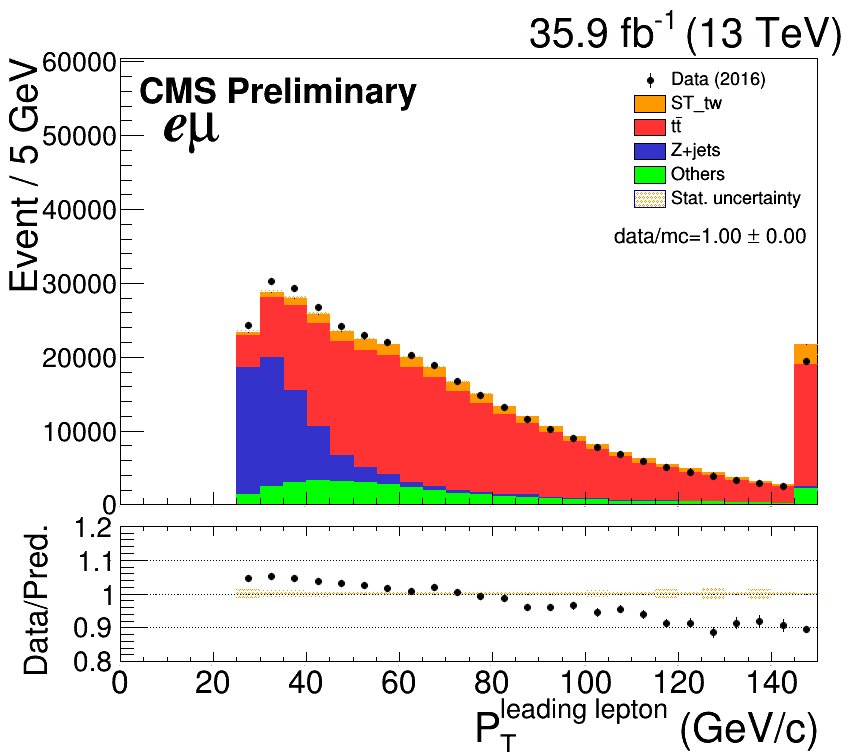
\includegraphics[width=0.32\textwidth]{figures/tW/fig/Step1/emu_noNvtx/H_lepton_led_pt.png}&
%      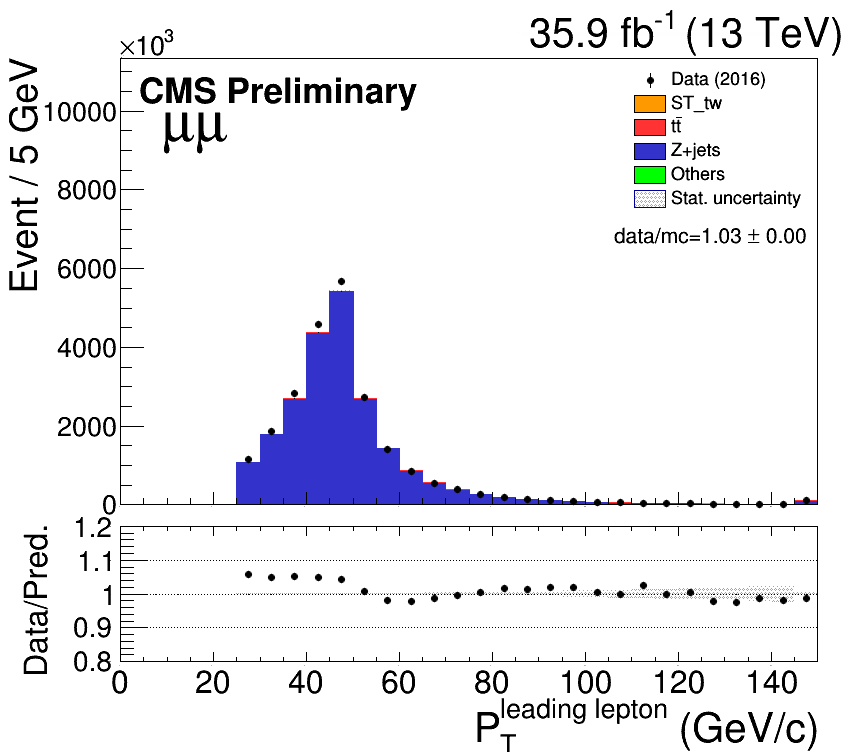
\includegraphics[width=0.32\textwidth]{figures/tW/fig/Step1/mumu_noNvtx/H_lepton_led_pt.png}\\
%      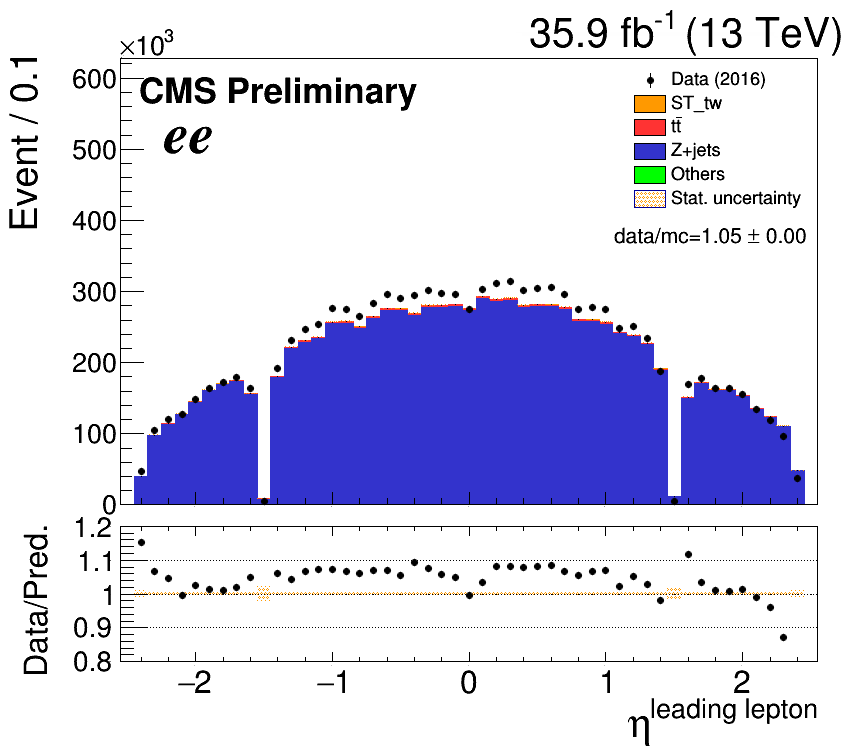
\includegraphics[width=0.32\textwidth]{figures/tW/fig/Step1/ee_noNvtx/H_lepton_led_eta.png}&
%      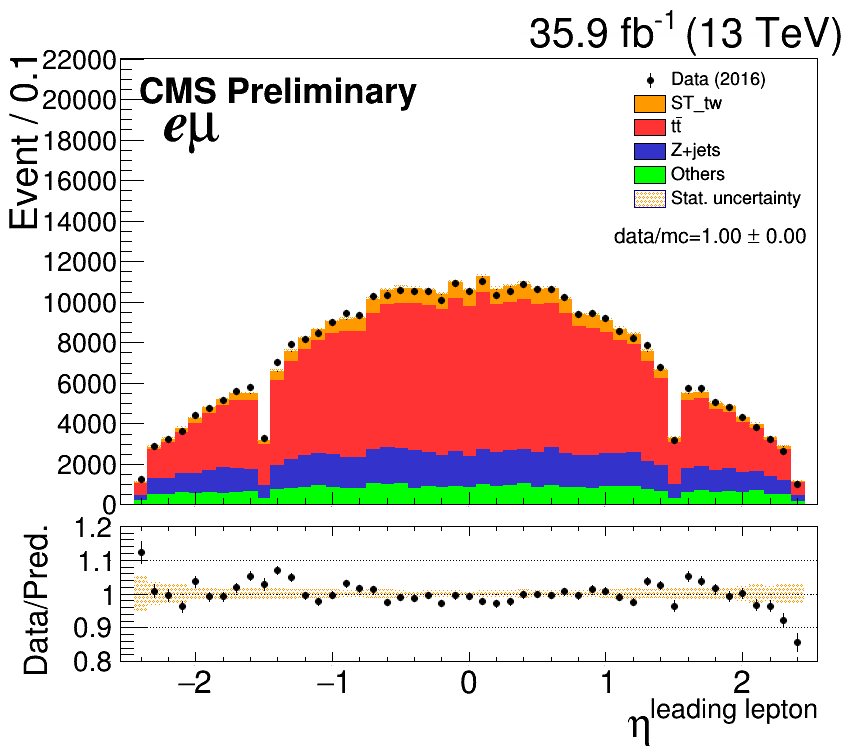
\includegraphics[width=0.32\textwidth]{figures/tW/fig/Step1/emu_noNvtx/H_lepton_led_eta.png}&
%      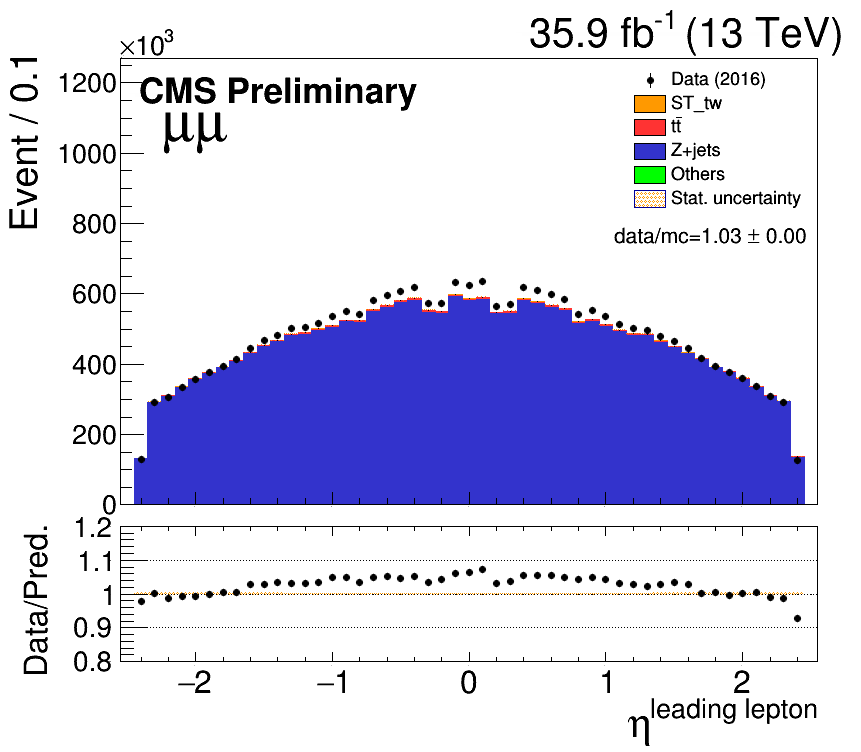
\includegraphics[width=0.32\textwidth]{figures/tW/fig/Step1/mumu_noNvtx/H_lepton_led_eta.png}\\
%      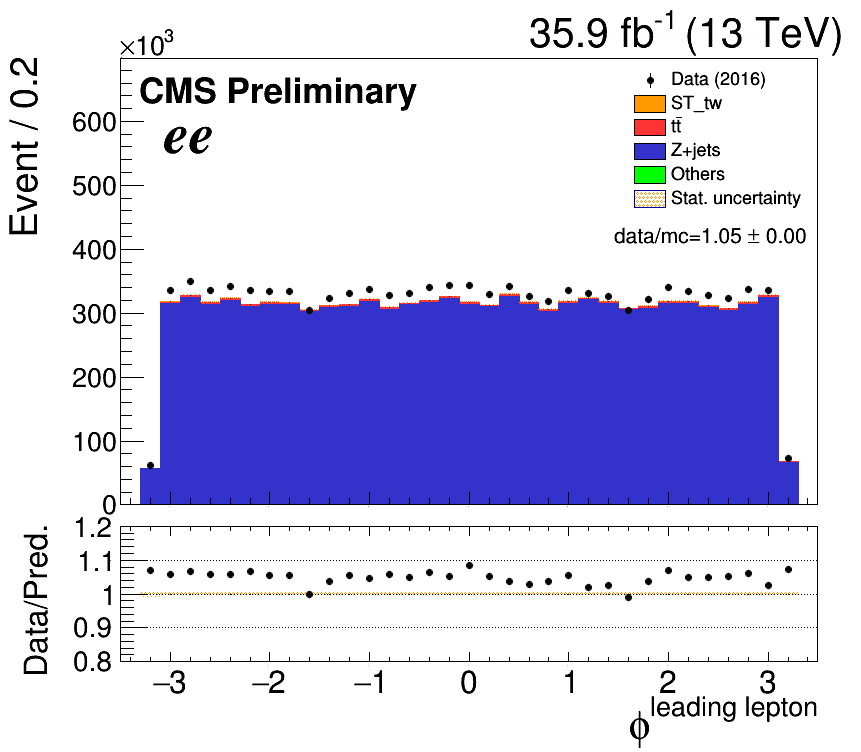
\includegraphics[width=0.32\textwidth]{figures/tW/fig/Step1/ee_noNvtx/H_lepton_led_phi.png}&
%      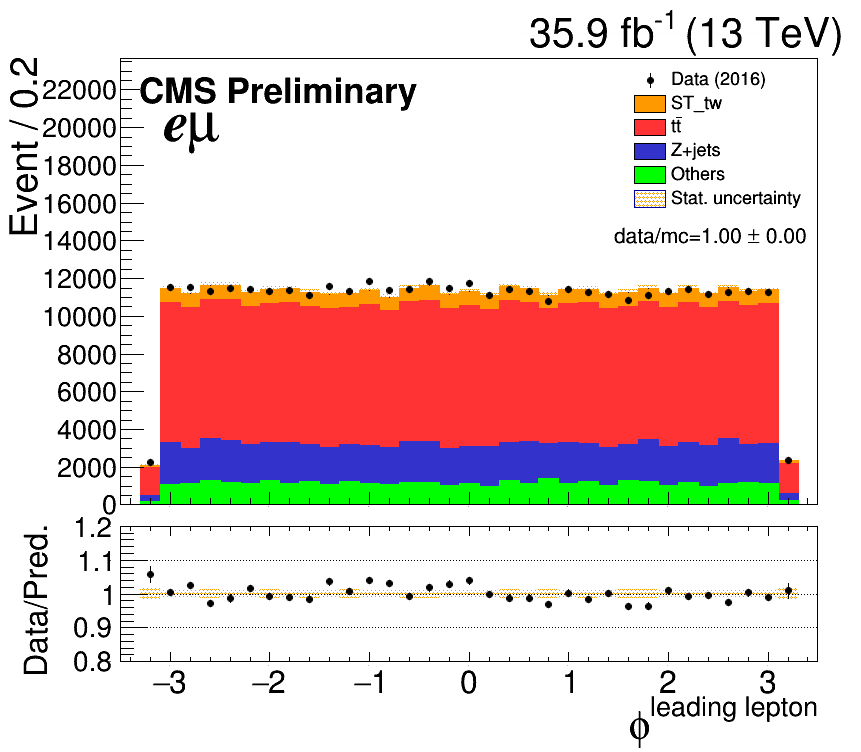
\includegraphics[width=0.32\textwidth]{figures/tW/fig/Step1/emu_noNvtx/H_lepton_led_phi.png}&
%      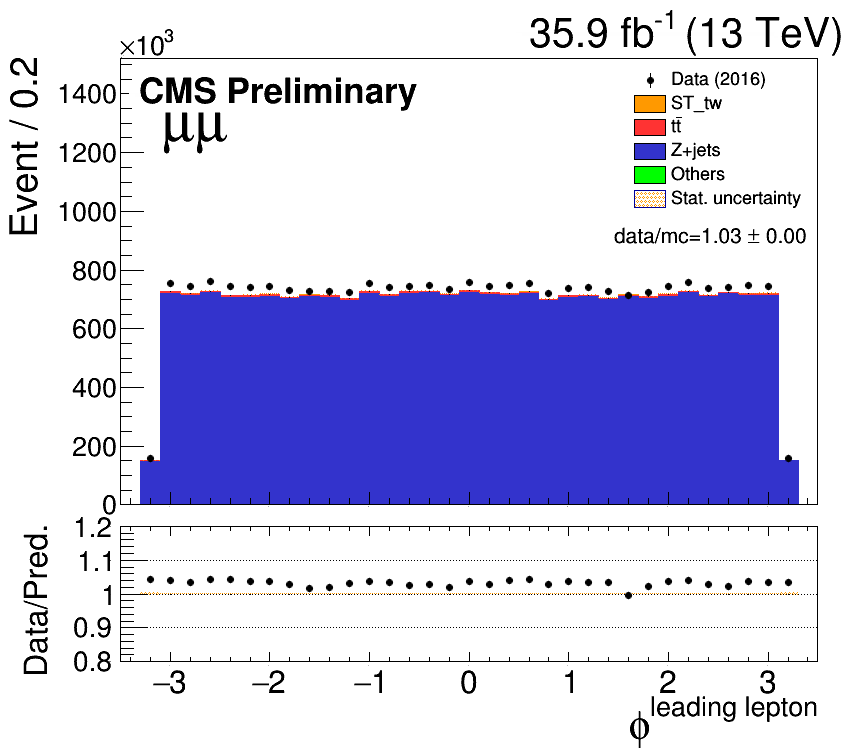
\includegraphics[width=0.32\textwidth]{figures/tW/fig/Step1/mumu_noNvtx/H_lepton_led_phi.png}\\
%    \end{tabular}
%    \caption{The distributions of Pt (top), $\eta$ (middle) and $\phi$ (bottom) of leading lepton for ee (left), $e\mu$ (middle) and \mumu (right) channels after step 1 (trigger and lepton selections). All backgrounds are estimated from MC.}
%    \label{fig:step1_leading_lepton1}
%  \end{center}
%\end{figure}
%
%\begin{figure}[ht]
%  \begin{center}
%    \begin{tabular}{ccc}
%      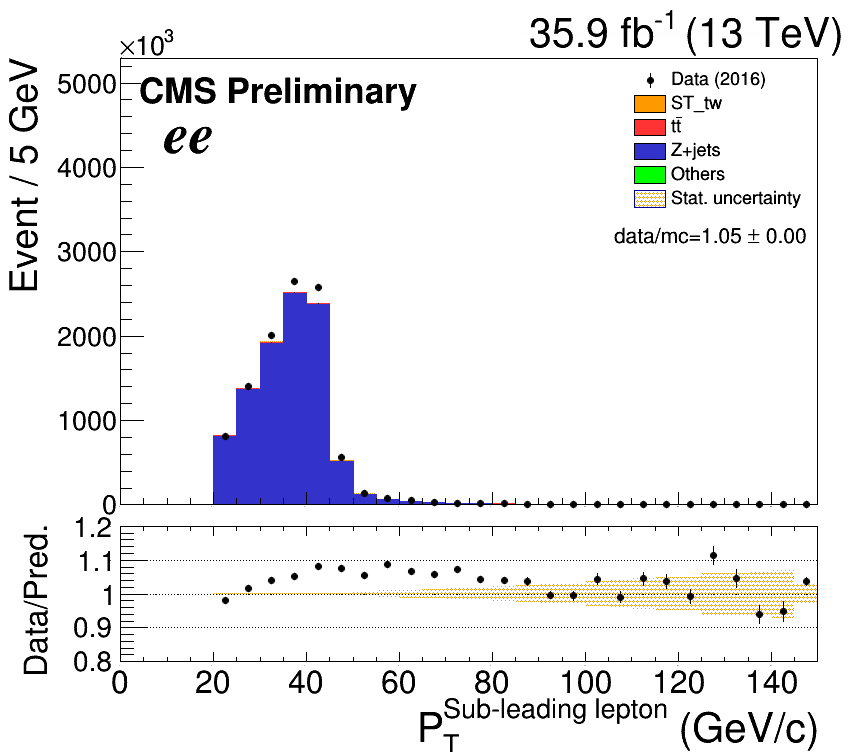
\includegraphics[width=0.32\textwidth]{figures/tW/fig/Step1/ee_noNvtx/H_lepton_sub_pt.png}&
%      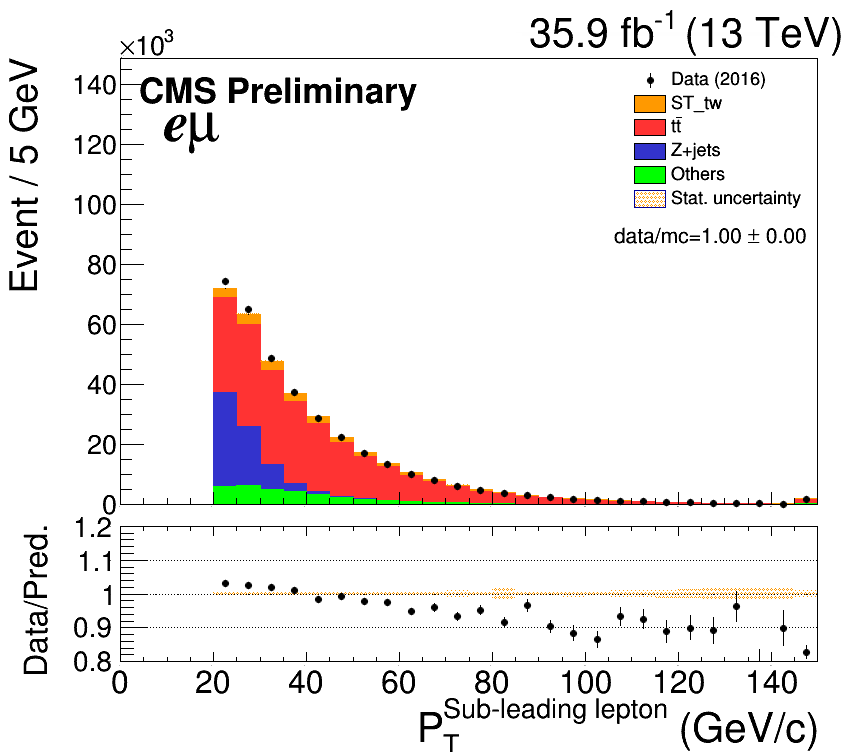
\includegraphics[width=0.32\textwidth]{figures/tW/fig/Step1/emu_noNvtx/H_lepton_sub_pt.png}&
%      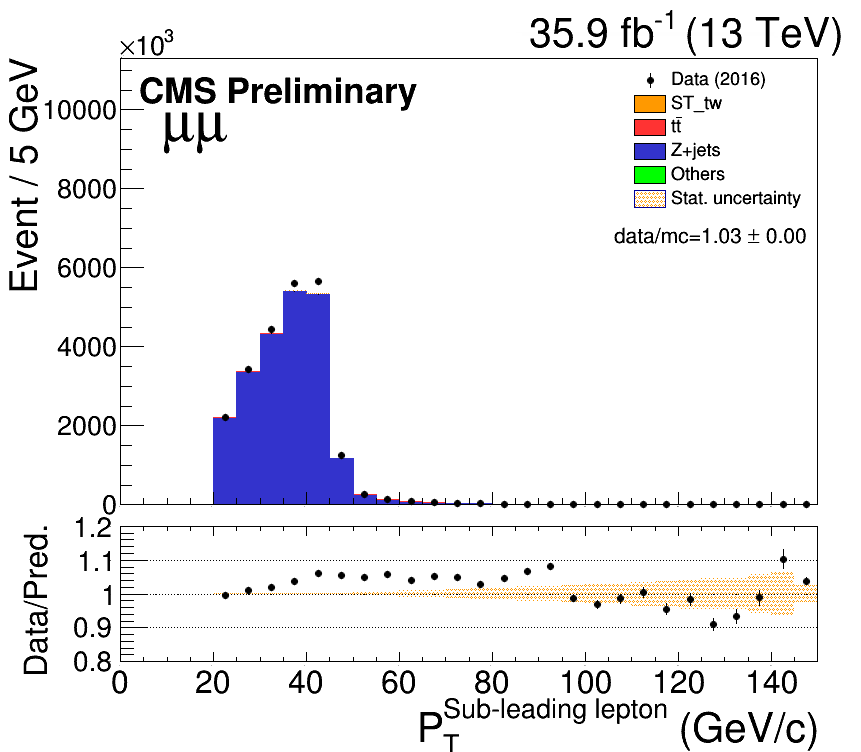
\includegraphics[width=0.32\textwidth]{figures/tW/fig/Step1/mumu_noNvtx/H_lepton_sub_pt.png}\\
%      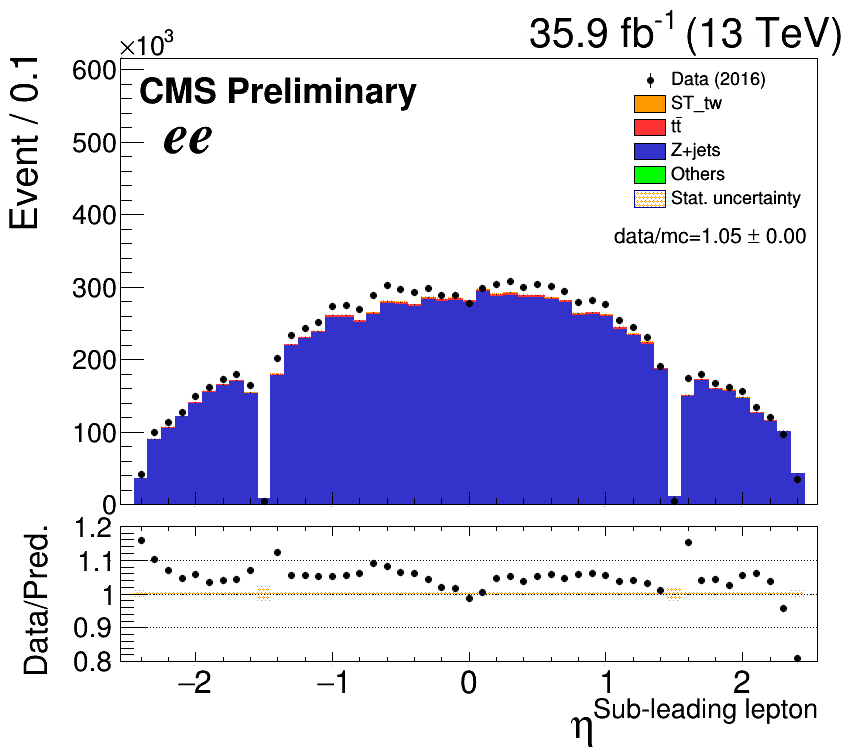
\includegraphics[width=0.32\textwidth]{figures/tW/fig/Step1/ee_noNvtx/H_lepton_sub_eta.png}&
%      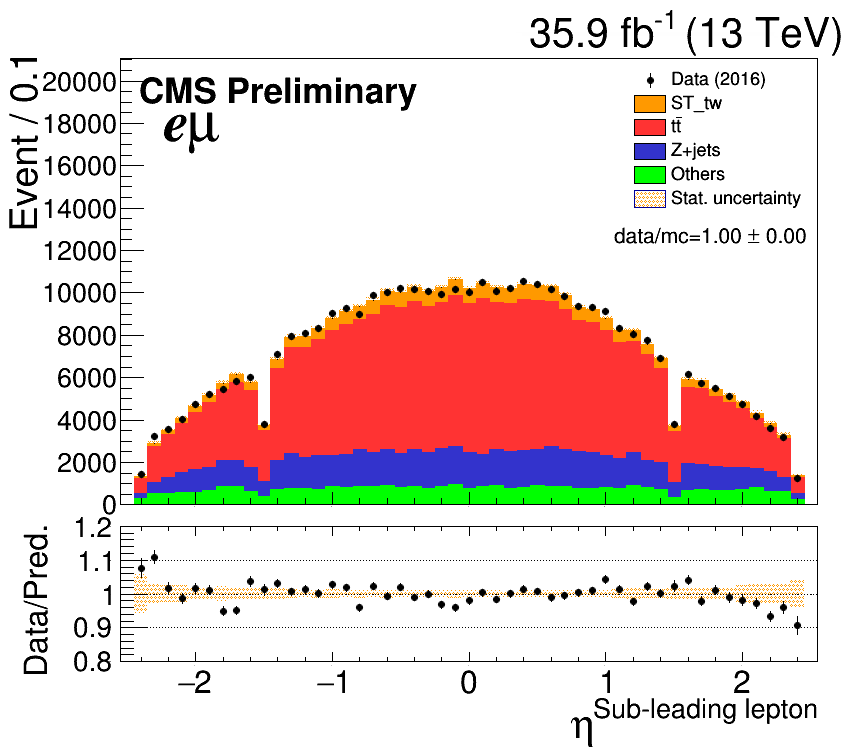
\includegraphics[width=0.32\textwidth]{figures/tW/fig/Step1/emu_noNvtx/H_lepton_sub_eta.png}&
%      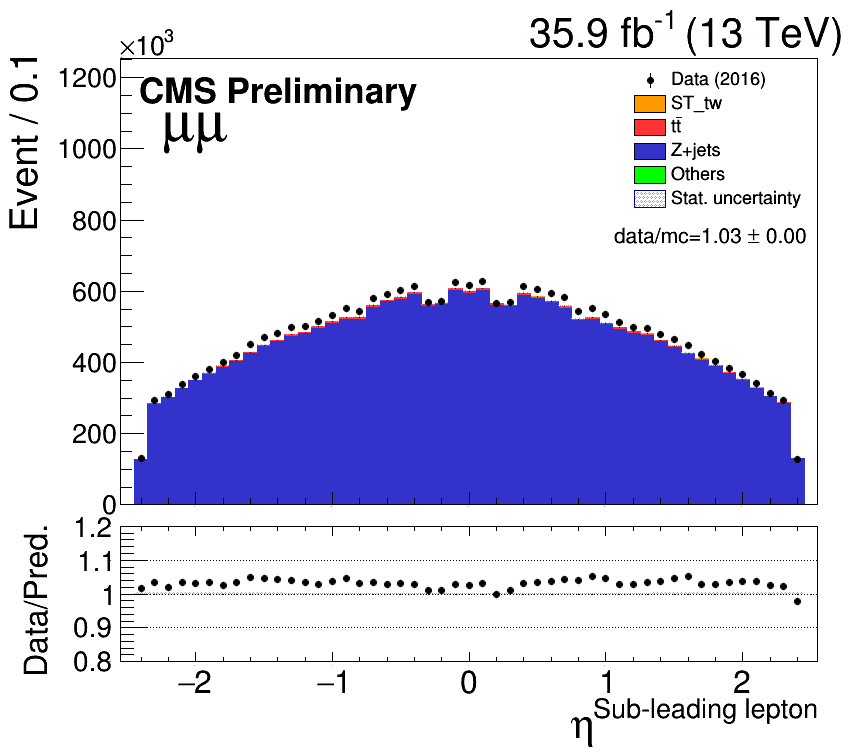
\includegraphics[width=0.32\textwidth]{figures/tW/fig/Step1/mumu_noNvtx/H_lepton_sub_eta.png}\\
%      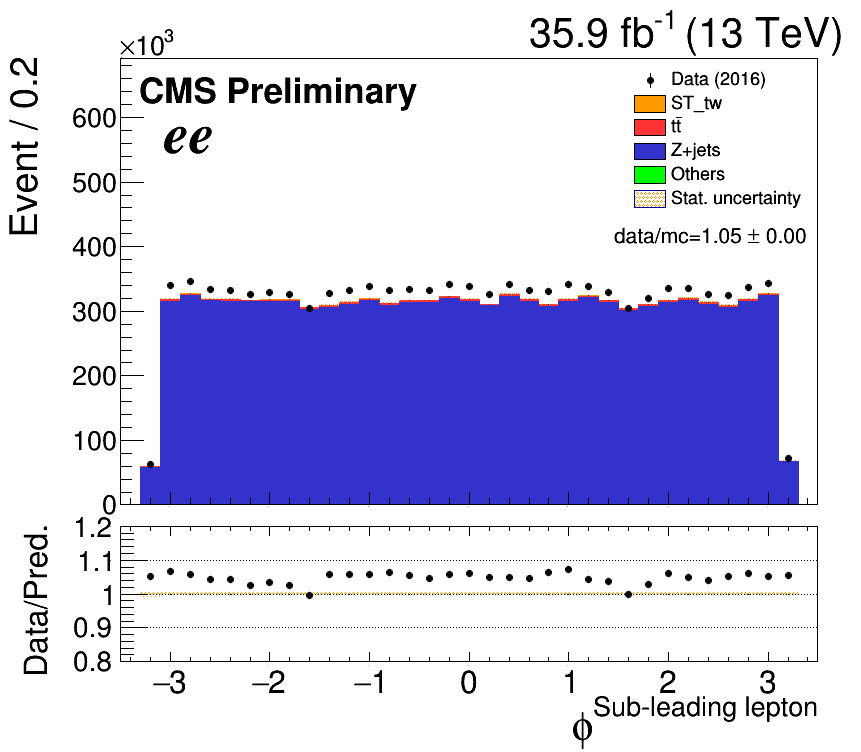
\includegraphics[width=0.32\textwidth]{figures/tW/fig/Step1/ee_noNvtx/H_lepton_sub_phi.png}&
%      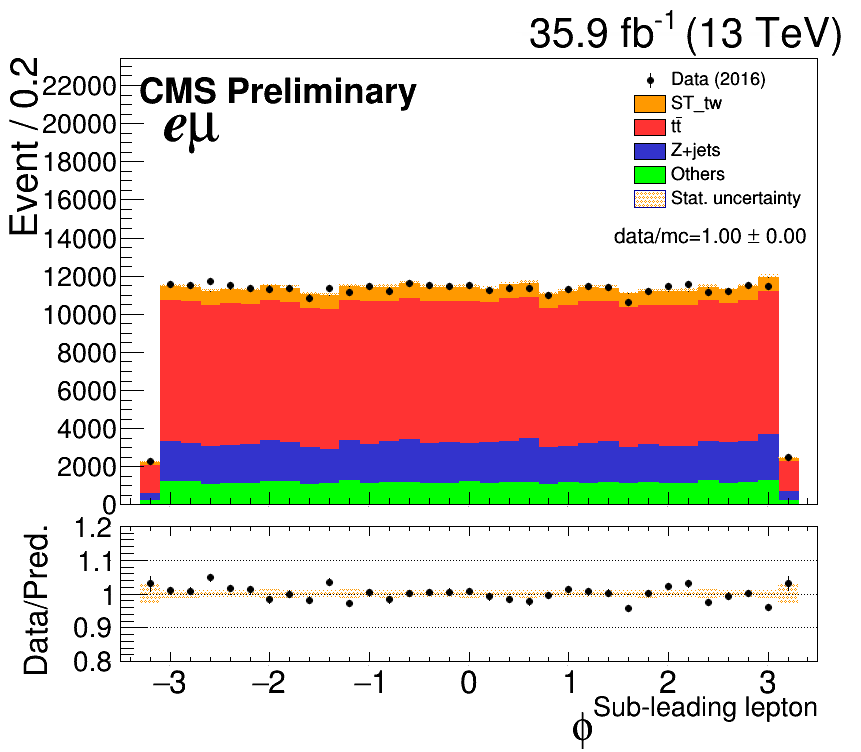
\includegraphics[width=0.32\textwidth]{figures/tW/fig/Step1/emu_noNvtx/H_lepton_sub_phi.png}&
%      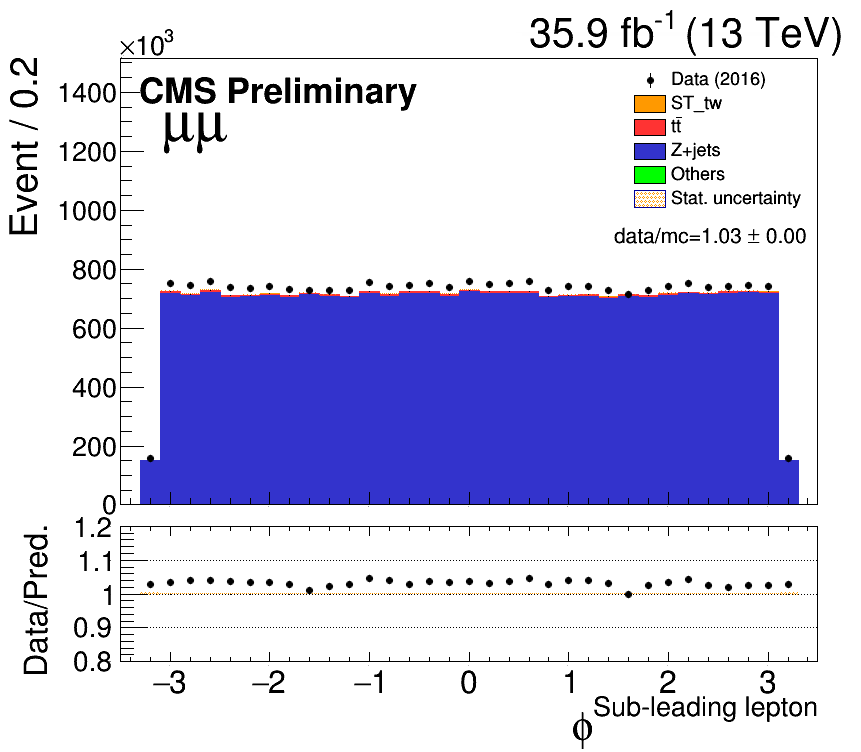
\includegraphics[width=0.32\textwidth]{figures/tW/fig/Step1/mumu_noNvtx/H_lepton_sub_phi.png}\\
%    \end{tabular}
%    \caption{The distributions of Pt (top), $\eta$ (middle) and $\phi$ (bottom) of sub-leading lepton for ee (left), $e\mu$ (middle) and \mumu (right) channels after step 1 (trigger and lepton selections). All backgrounds are estimated from MC.}
%    \label{fig:step1_leading_lepton}
%  \end{center}
%\end{figure}
%
%\begin{figure}[ht]
%  \begin{center}
%    \begin{tabular}{ccc}
%      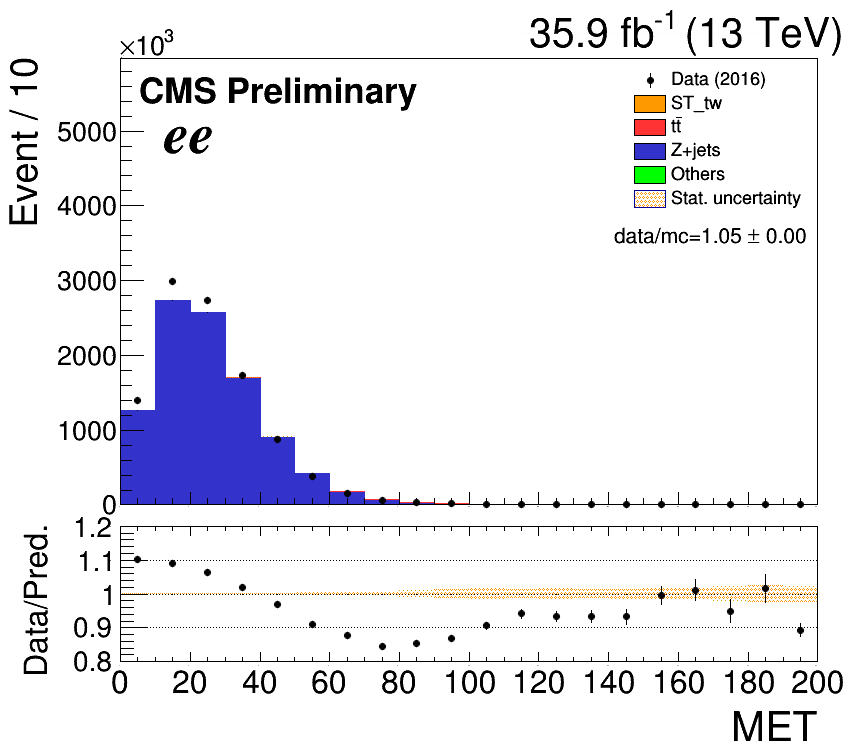
\includegraphics[width=0.32\textwidth]{figures/tW/fig/Step1/ee_noNvtx/H_MET_Et.png}&
%      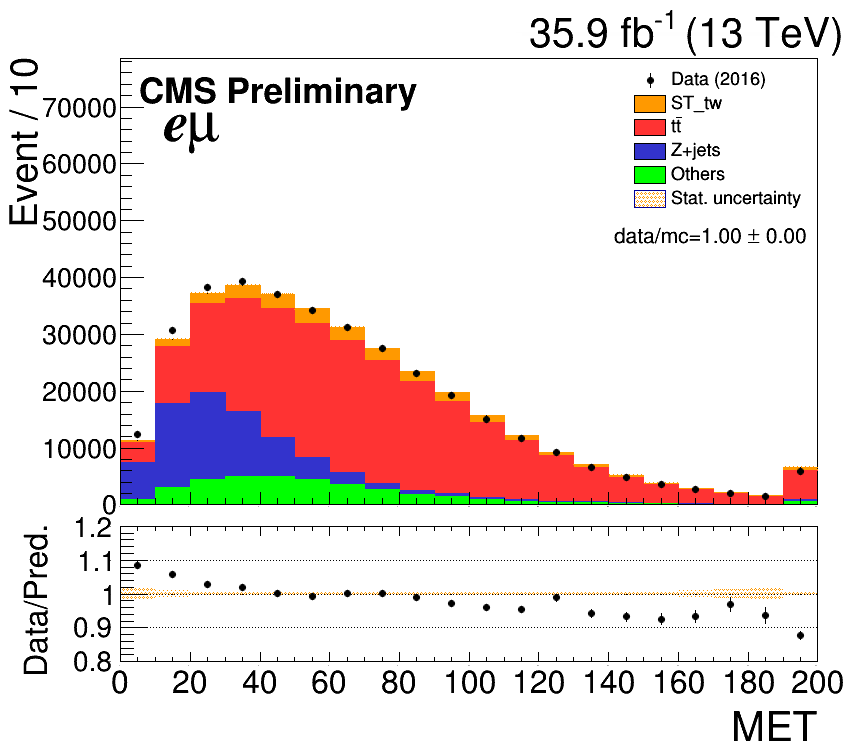
\includegraphics[width=0.32\textwidth]{figures/tW/fig/Step1/emu_noNvtx/H_MET_Et.png}&
%      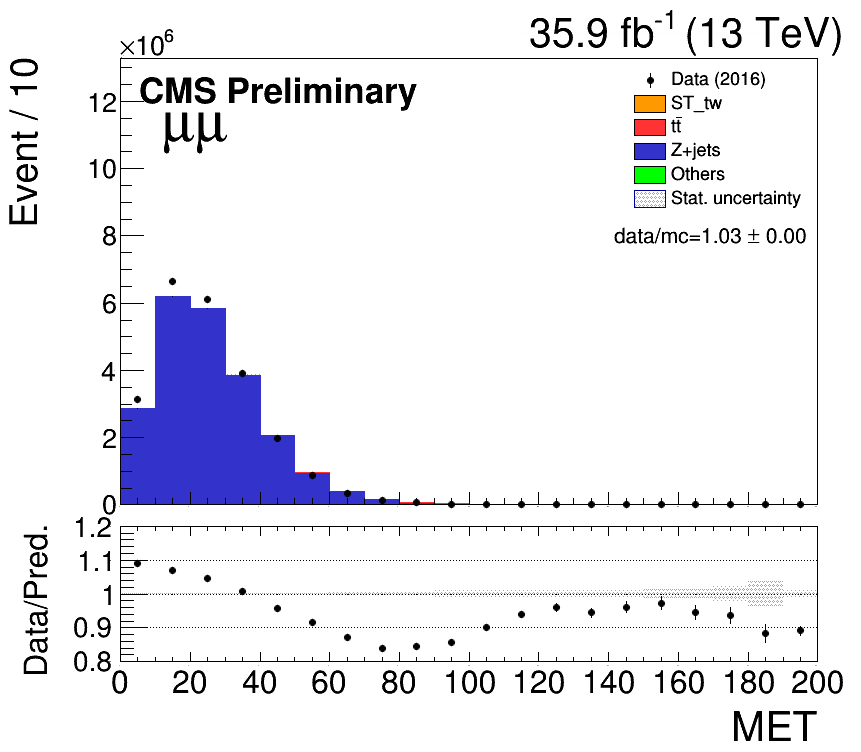
\includegraphics[width=0.32\textwidth]{figures/tW/fig/Step1/mumu_noNvtx/H_MET_Et.png}\\
%      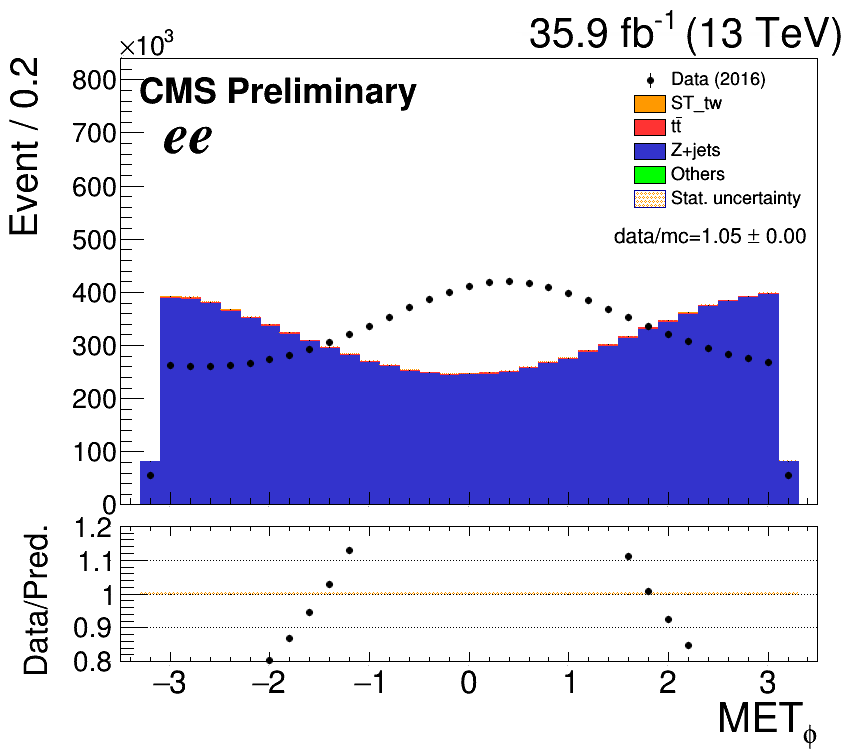
\includegraphics[width=0.32\textwidth]{figures/tW/fig/Step1/ee_noNvtx/H_MET_phi.png}&
%      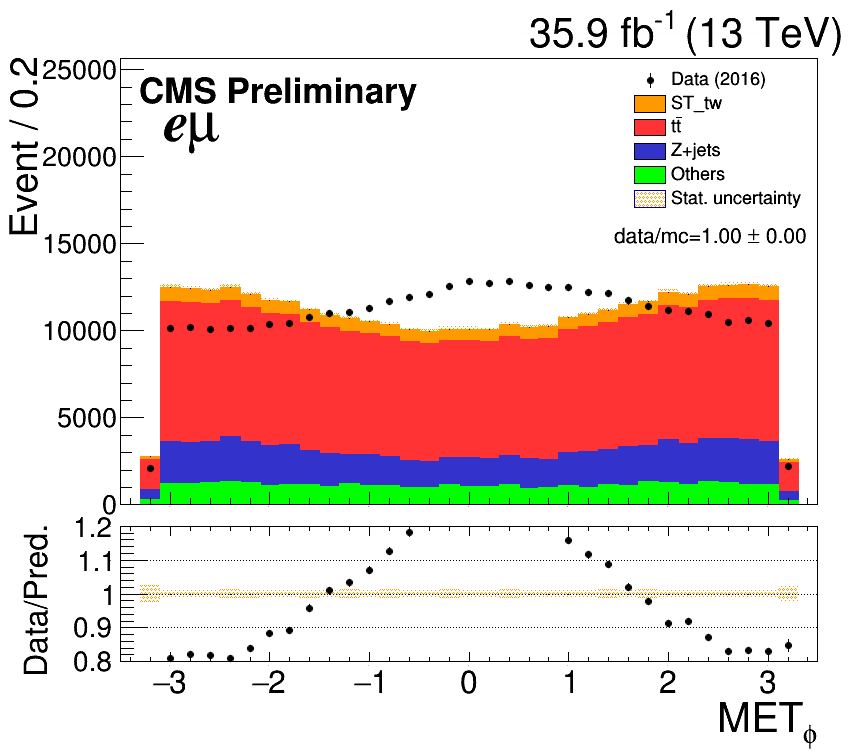
\includegraphics[width=0.32\textwidth]{figures/tW/fig/Step1/emu_noNvtx/H_MET_phi.png}&
%      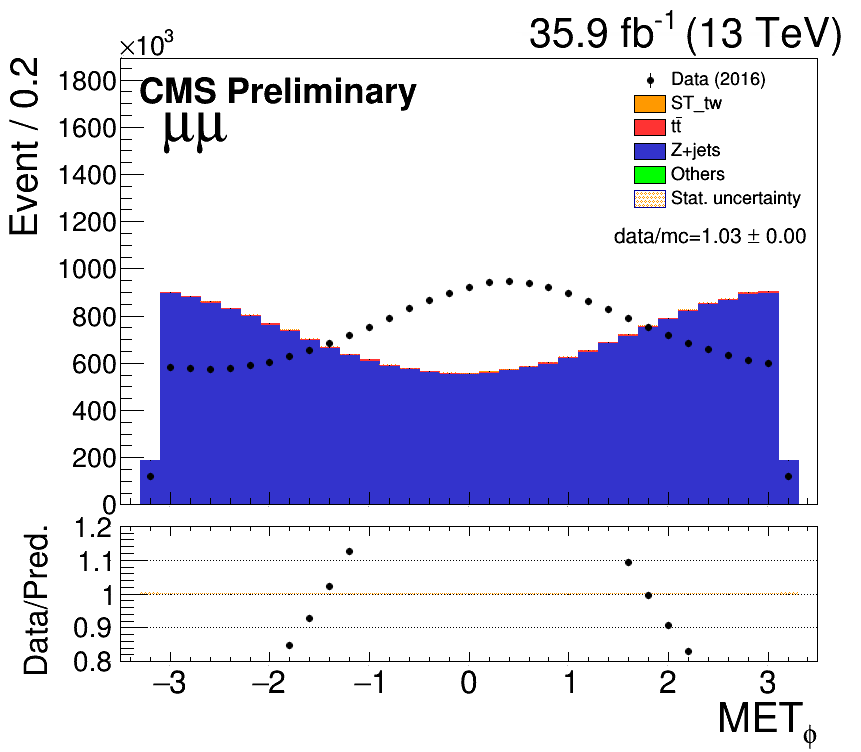
\includegraphics[width=0.32\textwidth]{figures/tW/fig/Step1/mumu_noNvtx/H_MET_phi.png}\\
%      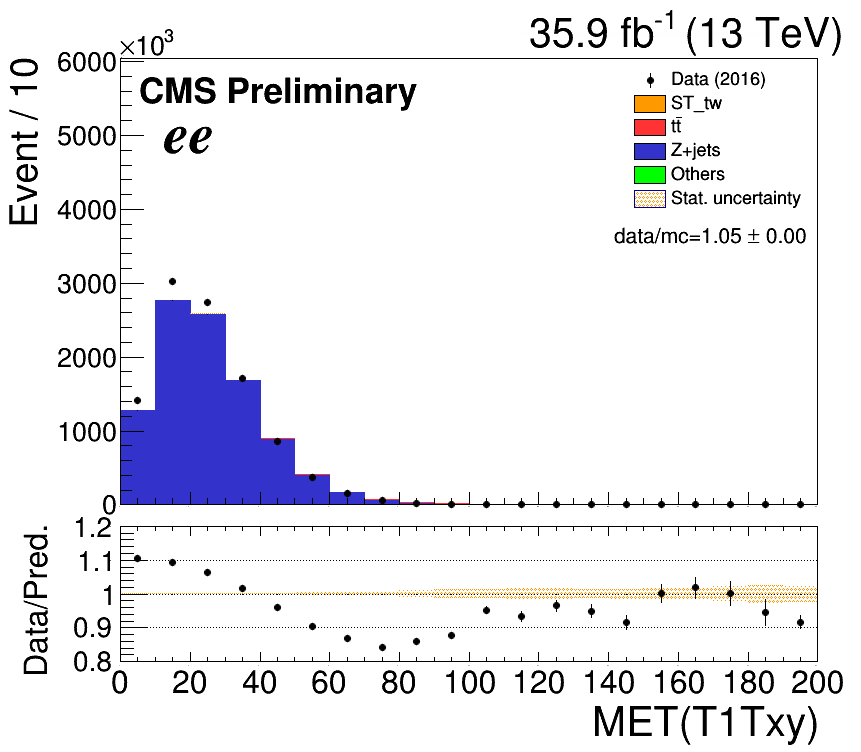
\includegraphics[width=0.32\textwidth]{figures/tW/fig/Step1/ee_noNvtx/H_MET_T1Txy_et.png}&
%      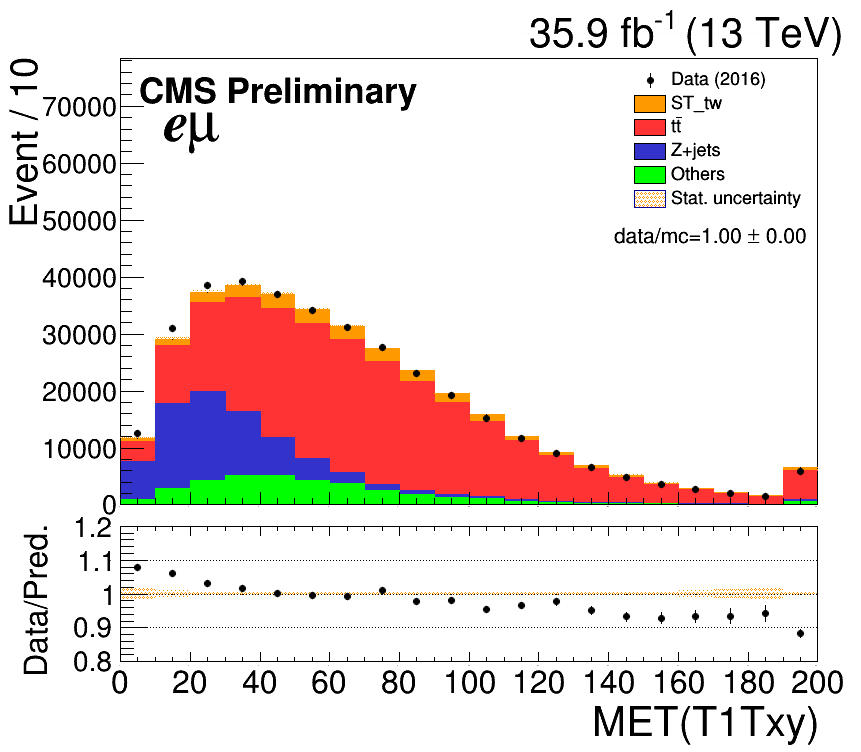
\includegraphics[width=0.32\textwidth]{figures/tW/fig/Step1/emu_noNvtx/H_MET_T1Txy_et.png}&
%      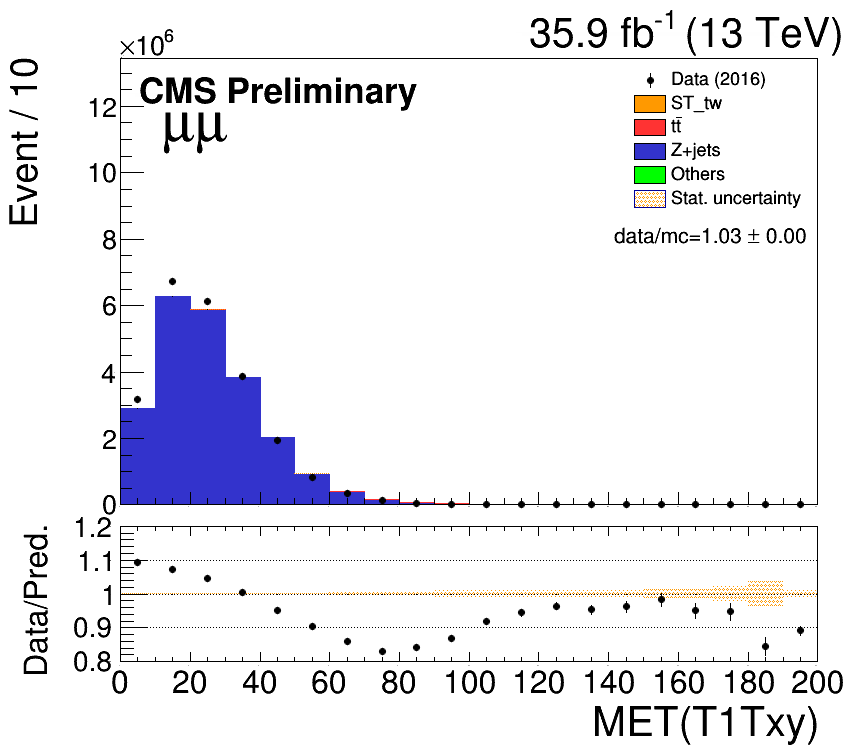
\includegraphics[width=0.32\textwidth]{figures/tW/fig/Step1/mumu_noNvtx/H_MET_T1Txy_et.png}\\
%      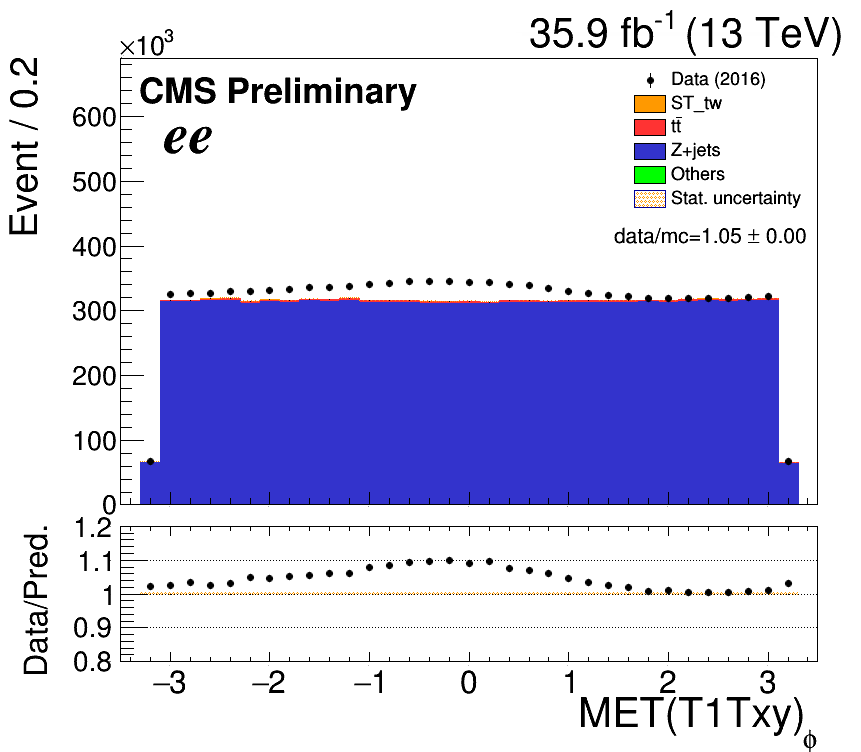
\includegraphics[width=0.32\textwidth]{figures/tW/fig/Step1/ee_noNvtx/H_MET_T1Txy_phi.png}&
%      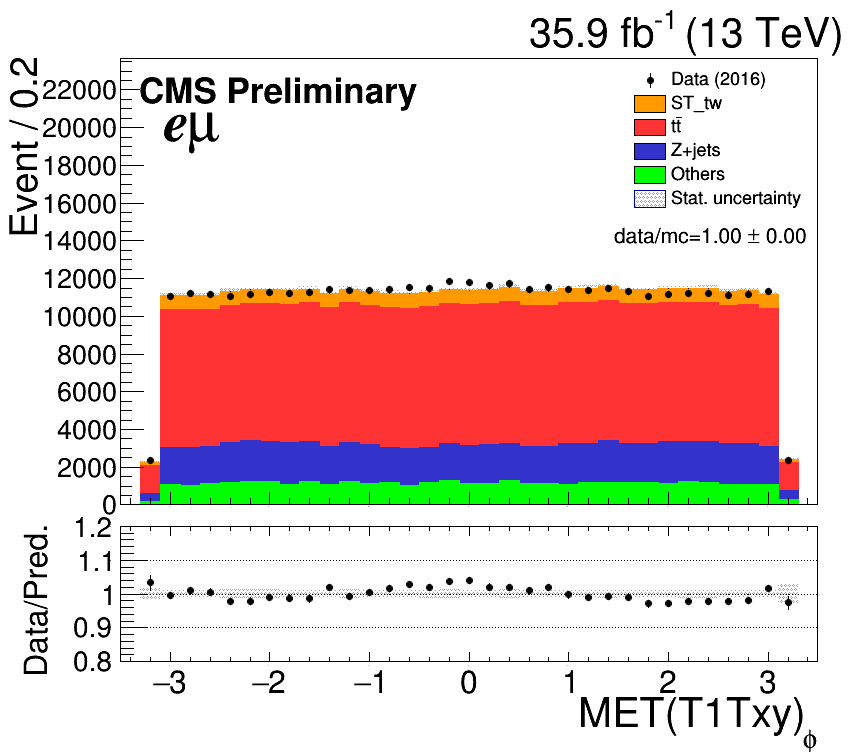
\includegraphics[width=0.32\textwidth]{figures/tW/fig/Step1/emu_noNvtx/H_MET_T1Txy_phi.png}&
%      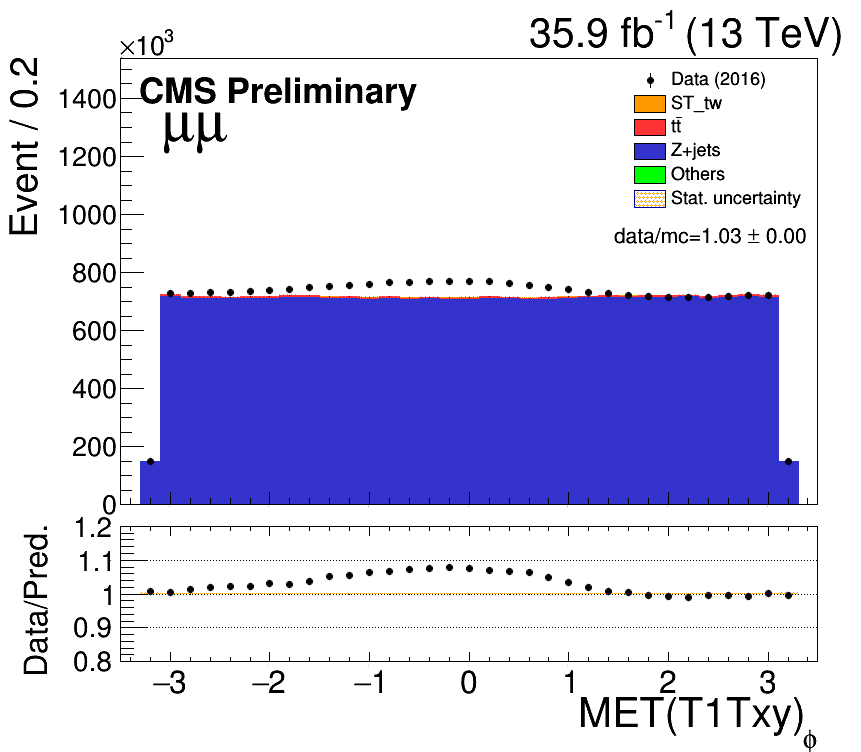
\includegraphics[width=0.32\textwidth]{figures/tW/fig/Step1/mumu_noNvtx/H_MET_T1Txy_phi.png}\\
%    \end{tabular}
%    \caption{The distributions of MET-T1 corrected (first row), $\phi$ of MET (second row), MET-T1-Txy corrected (third row) and $\phi$ of MET-T1-Txy corrected (last row) for ee (left), $e\mu$ (middle) and \mumu (right) channels after step 1 (trigger and lepton selections). All backgrounds are estimated from MC.}
%    \label{fig:step1_MET_phi}
%  \end{center}
%\end{figure}
%
%
%\begin{figure}[ht]
%  \begin{center}
%    \begin{tabular}{ccc}
%      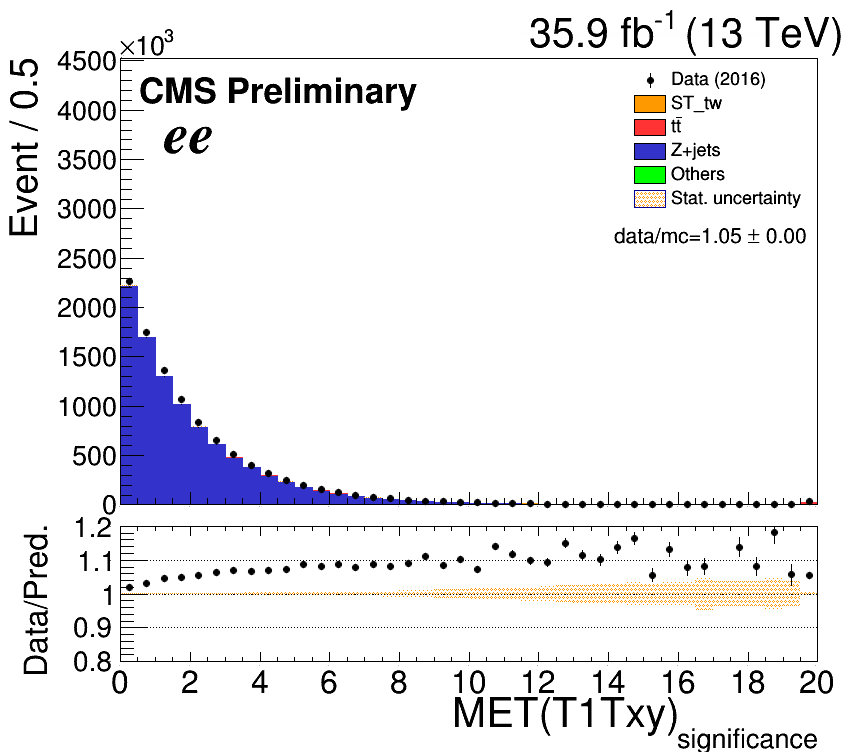
\includegraphics[width=0.32\textwidth]{figures/tW/fig/Step1/ee_noNvtx/H_MET_T1Txy_sf.png}&
%      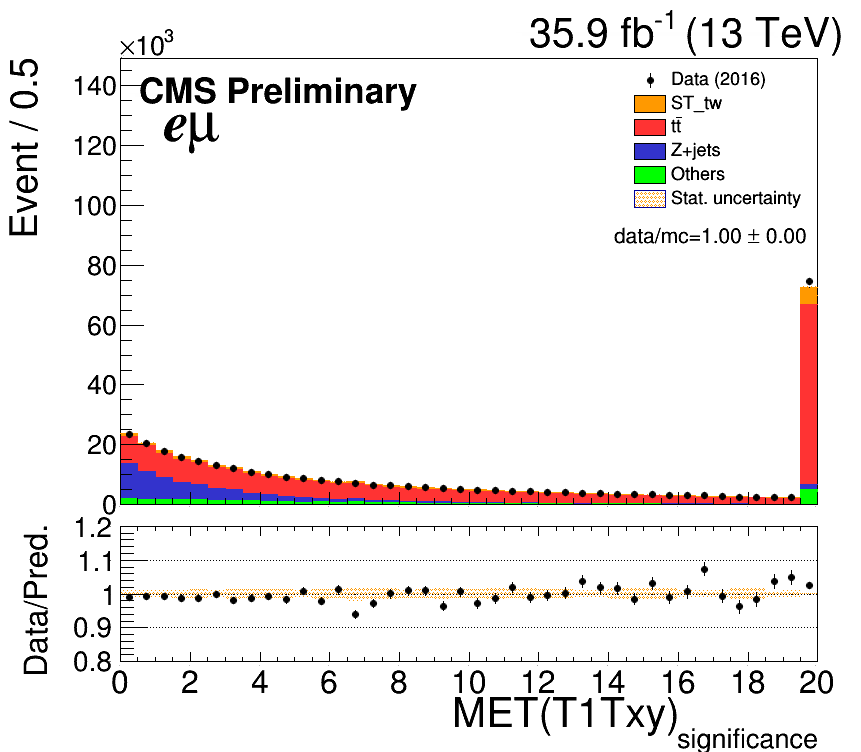
\includegraphics[width=0.32\textwidth]{figures/tW/fig/Step1/emu_noNvtx/H_MET_T1Txy_sf.png}&
%      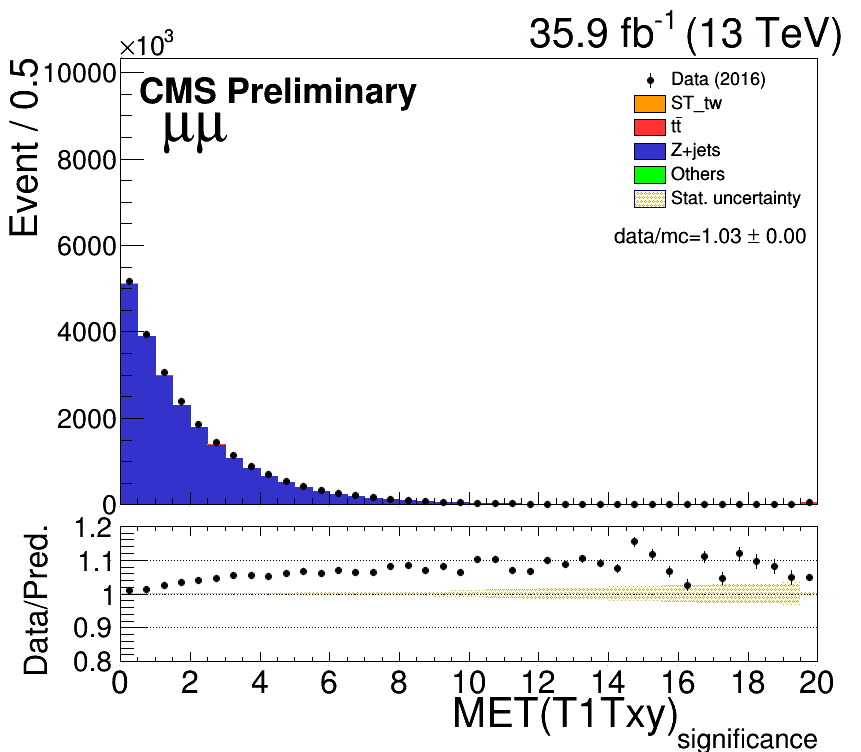
\includegraphics[width=0.32\textwidth]{figures/tW/fig/Step1/mumu_noNvtx/H_MET_T1Txy_sf.png}\\
%      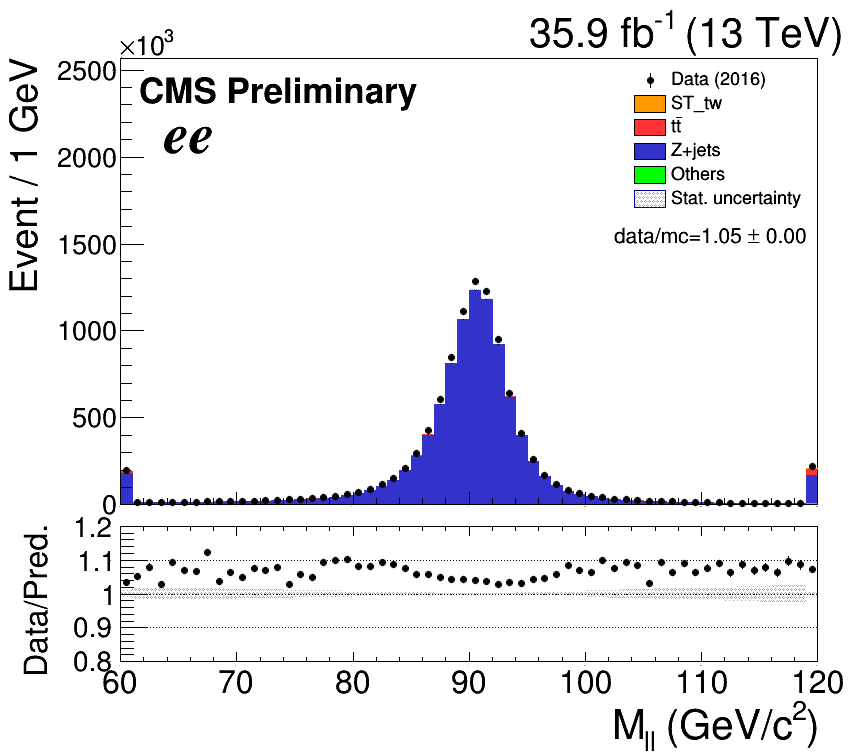
\includegraphics[width=0.32\textwidth]{figures/tW/fig/Step1/ee_noNvtx/H_Mll_Zpeak.png}&
%      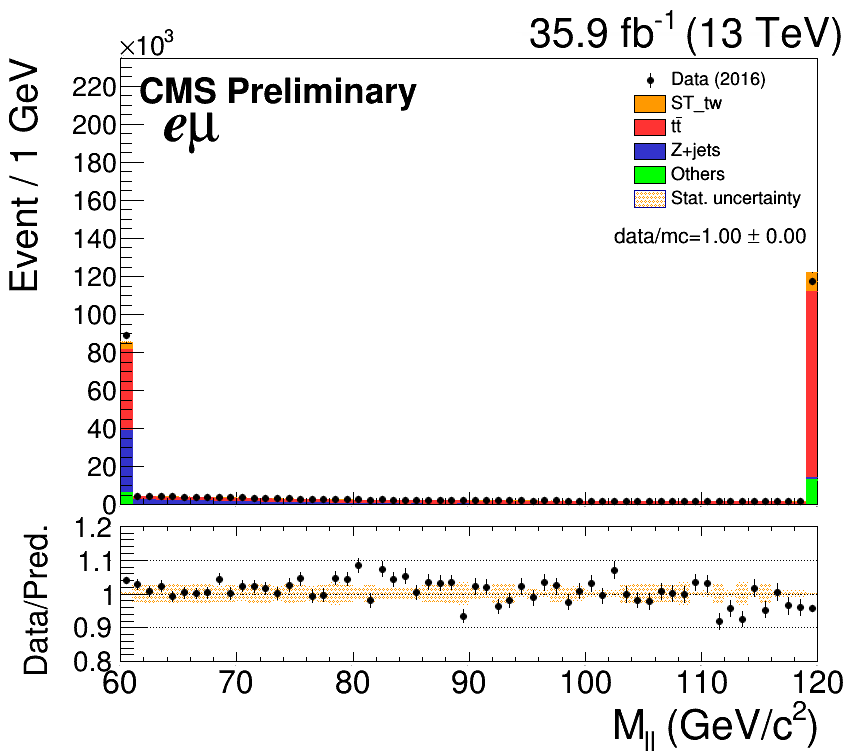
\includegraphics[width=0.32\textwidth]{figures/tW/fig/Step1/emu_noNvtx/H_Mll_Zpeak.png}&
%      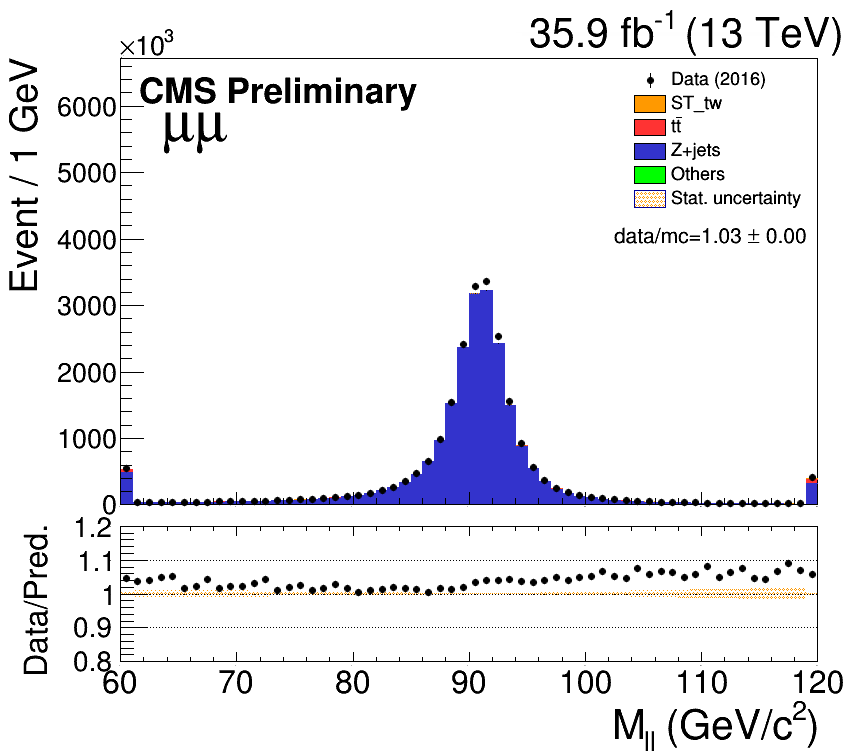
\includegraphics[width=0.32\textwidth]{figures/tW/fig/Step1/mumu_noNvtx/H_Mll_Zpeak.png}\\
%      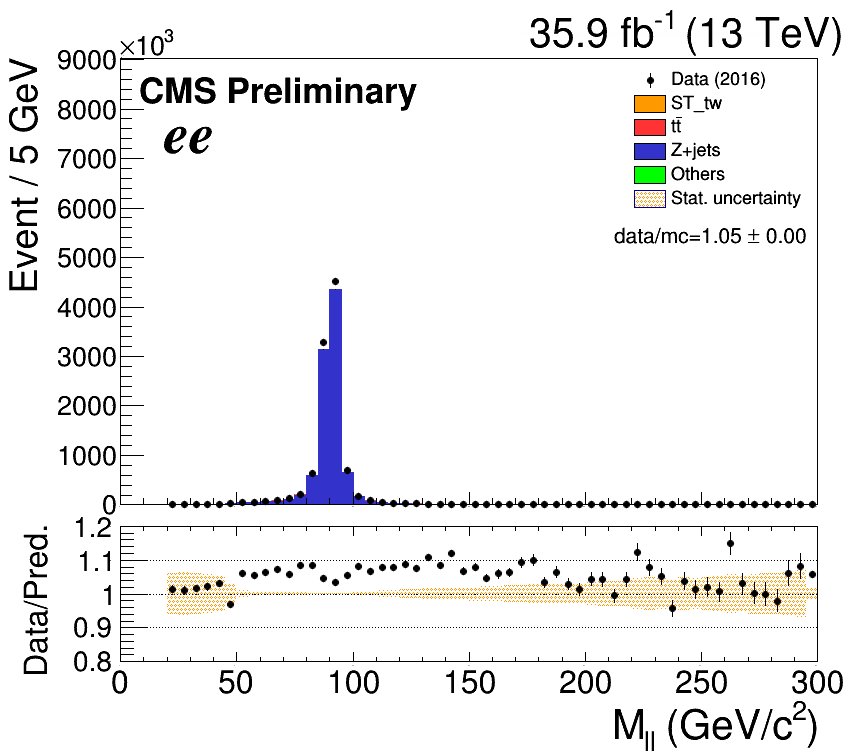
\includegraphics[width=0.32\textwidth]{figures/tW/fig/Step1/ee_noNvtx/H_Mll.png}&
%      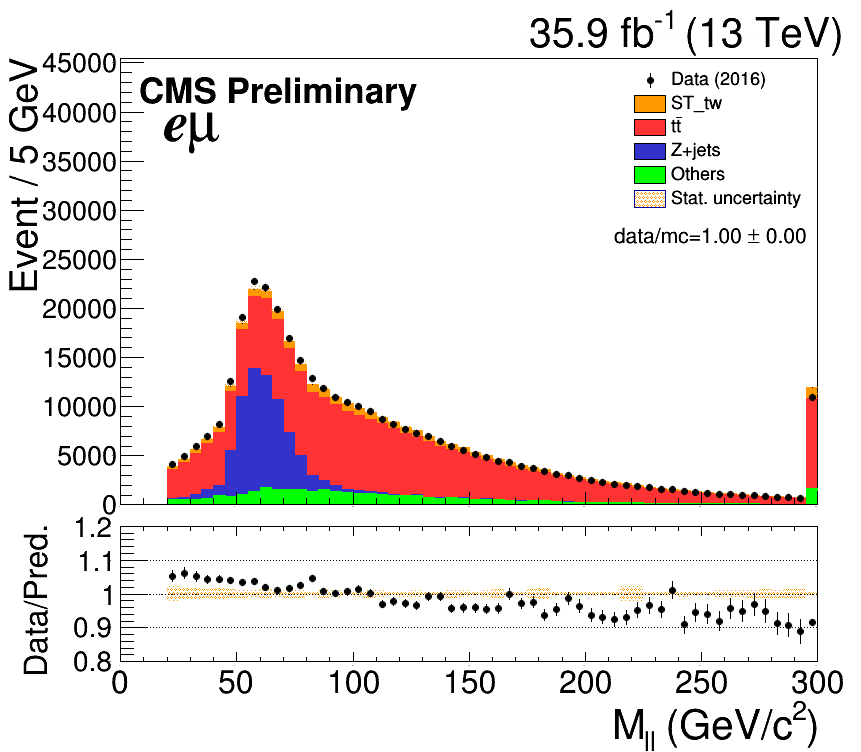
\includegraphics[width=0.32\textwidth]{figures/tW/fig/Step1/emu_noNvtx/H_Mll.png}&
%      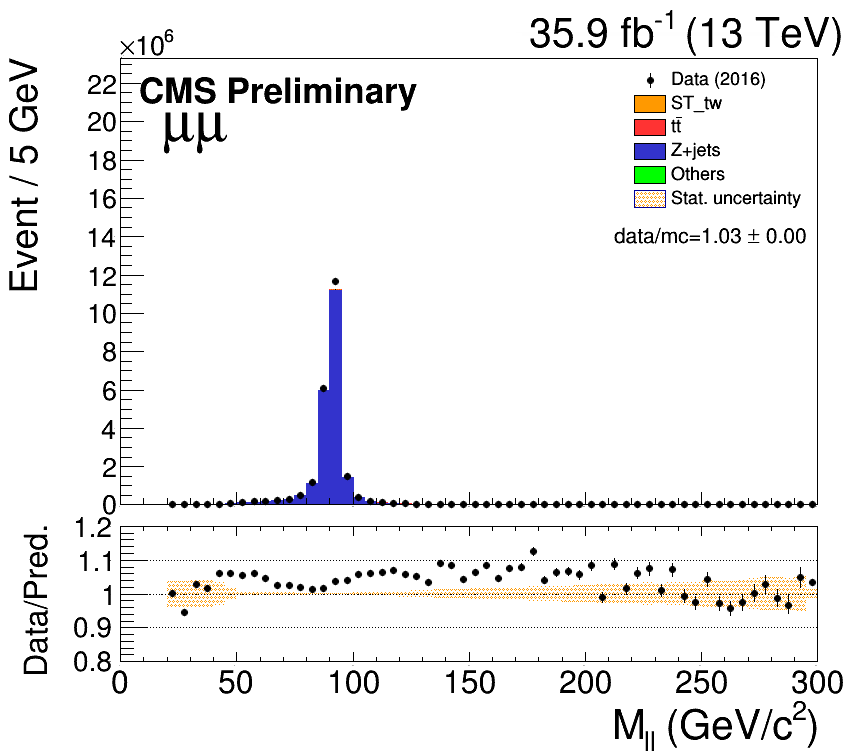
\includegraphics[width=0.32\textwidth]{figures/tW/fig/Step1/mumu_noNvtx/H_Mll.png}\\
%      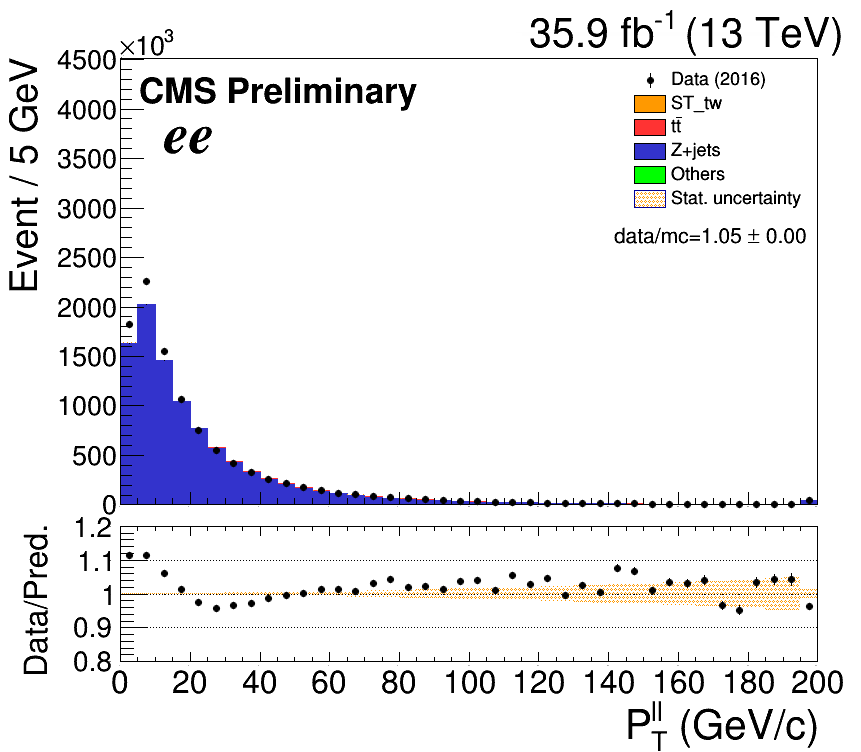
\includegraphics[width=0.32\textwidth]{figures/tW/fig/Step1/ee_noNvtx/H_Ptll.png}&
%      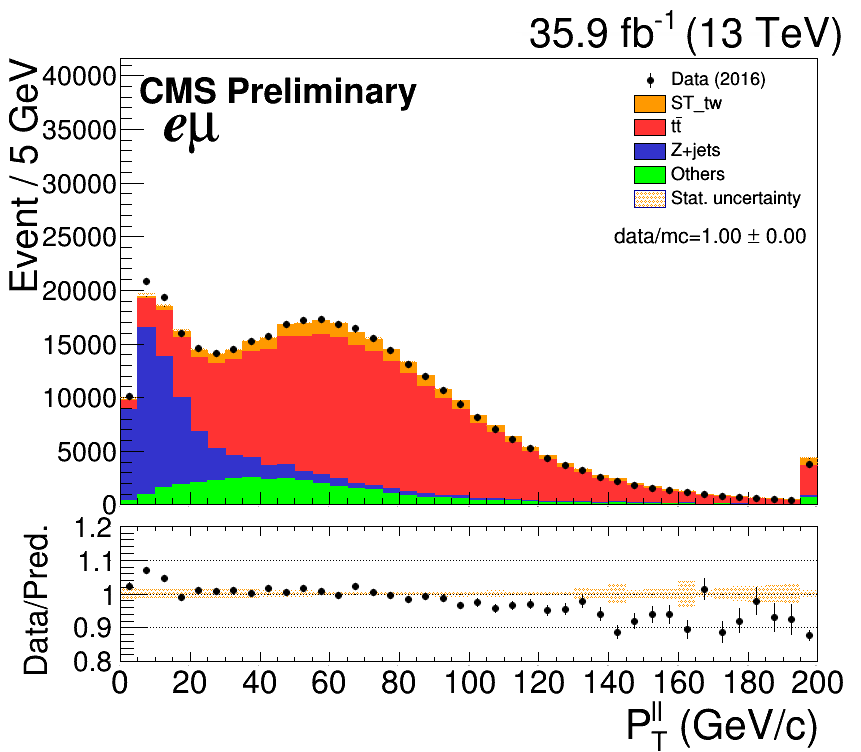
\includegraphics[width=0.32\textwidth]{figures/tW/fig/Step1/emu_noNvtx/H_Ptll.png}&
%      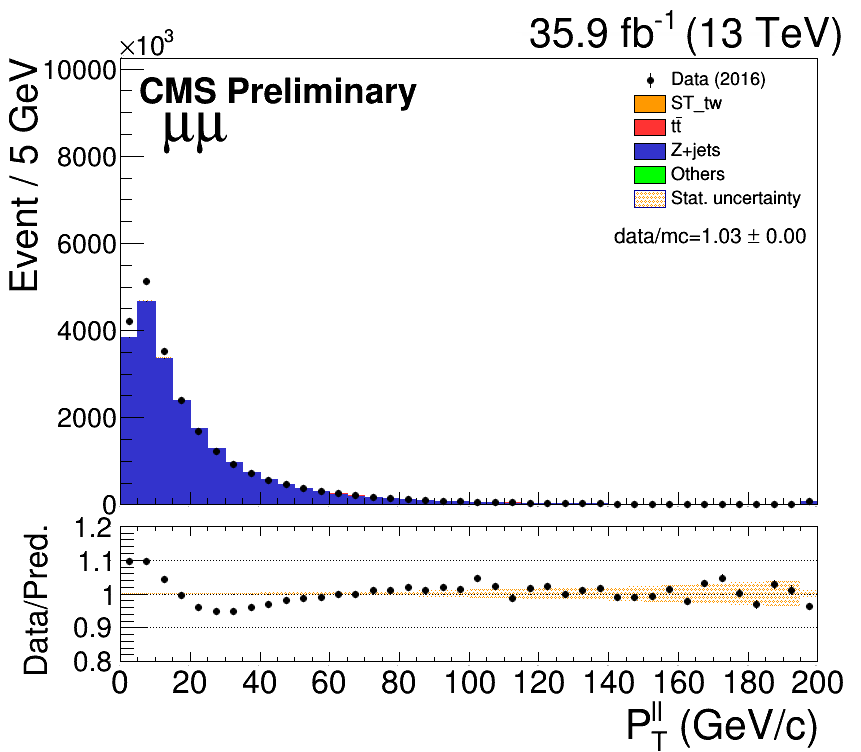
\includegraphics[width=0.32\textwidth]{figures/tW/fig/Step1/mumu_noNvtx/H_Ptll.png}\\
%    \end{tabular}
%    \caption{The distributions of MET significance (first row), invariant mass of two leptons in Z peak region [60-120] (second row), invariant mass of two leptons in wide range (third row) and Pt of two leptons system (last row) for ee (left), $e\mu$ (middle) and \mumu (right) channels after step 1 (trigger and lepton selections). All backgrounds are estimated from MC.}
%    \label{fig:step1_METsf_M_pt}
%  \end{center}
%\end{figure}
%
%\begin{figure}[ht]
%  \begin{center}
%    \begin{tabular}{ccc}
%      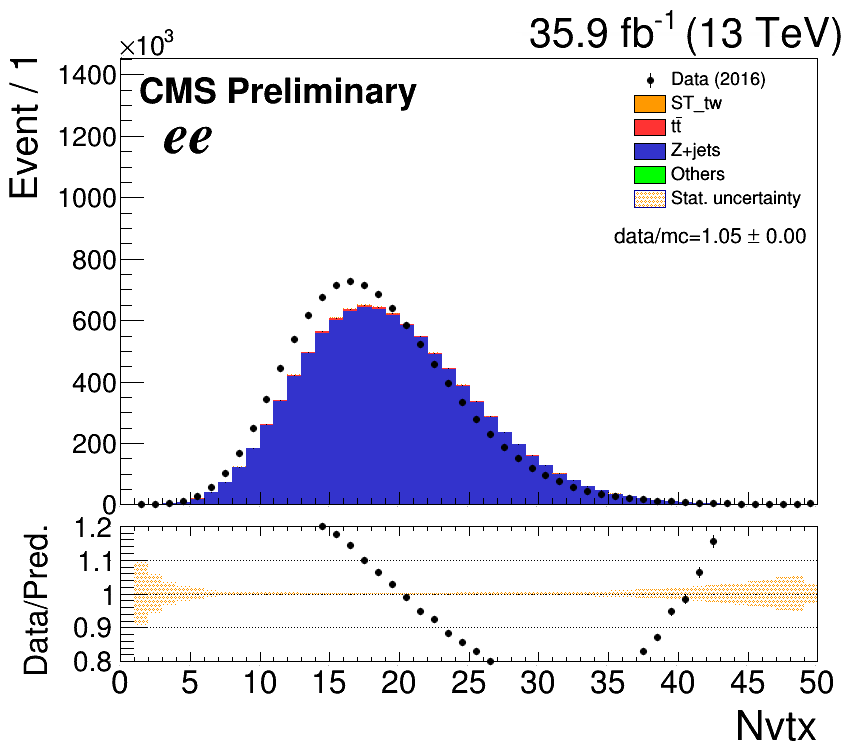
\includegraphics[width=0.32\textwidth]{figures/tW/fig/Step1/ee_noNvtx/H_pv_n.png}&
%      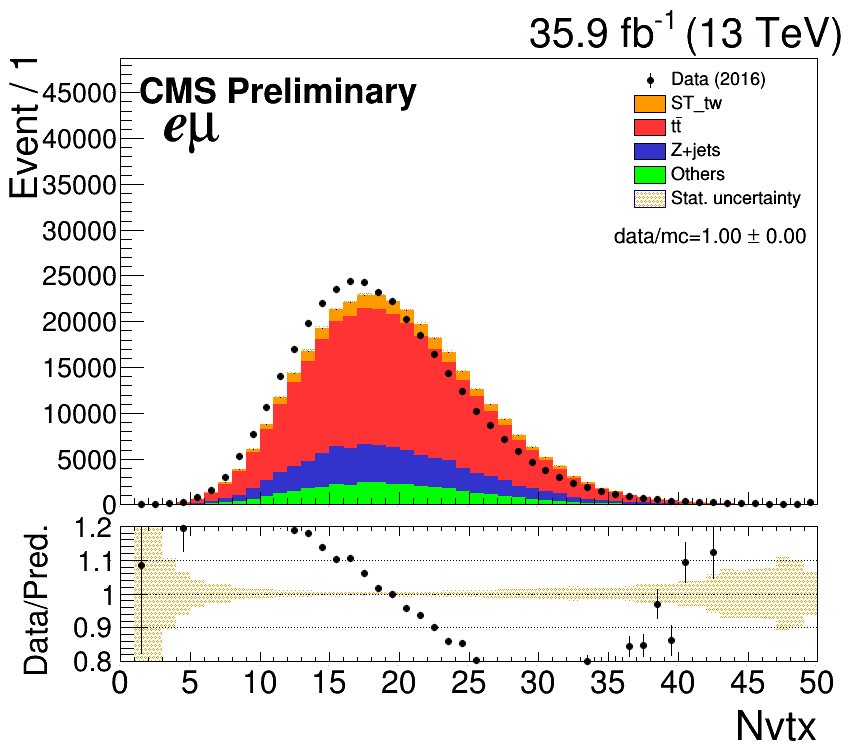
\includegraphics[width=0.32\textwidth]{figures/tW/fig/Step1/emu_noNvtx/H_pv_n.png}&
%      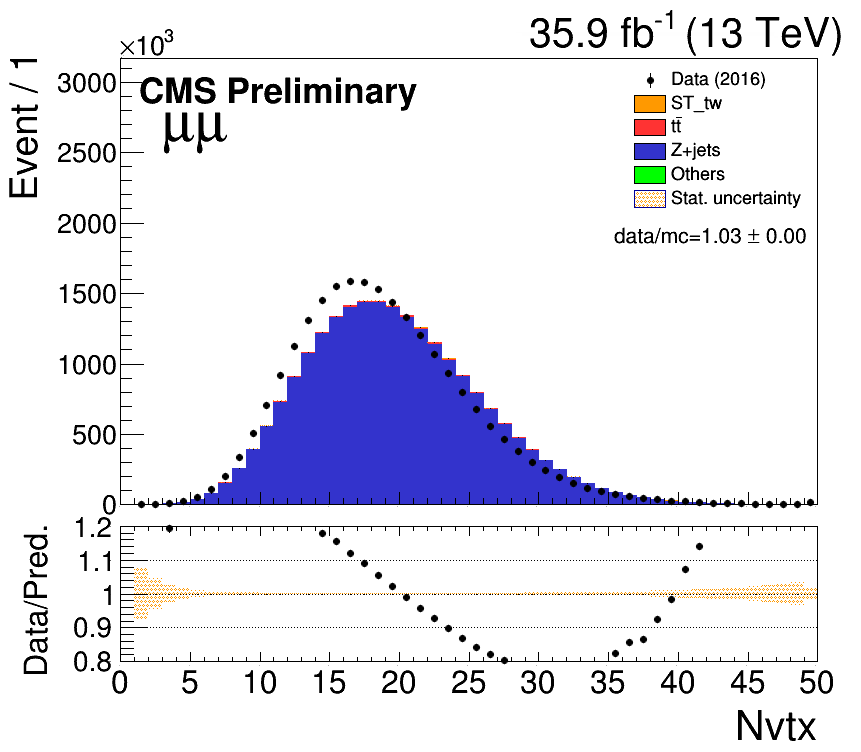
\includegraphics[width=0.32\textwidth]{figures/tW/fig/Step1/mumu_noNvtx/H_pv_n.png}\\
%      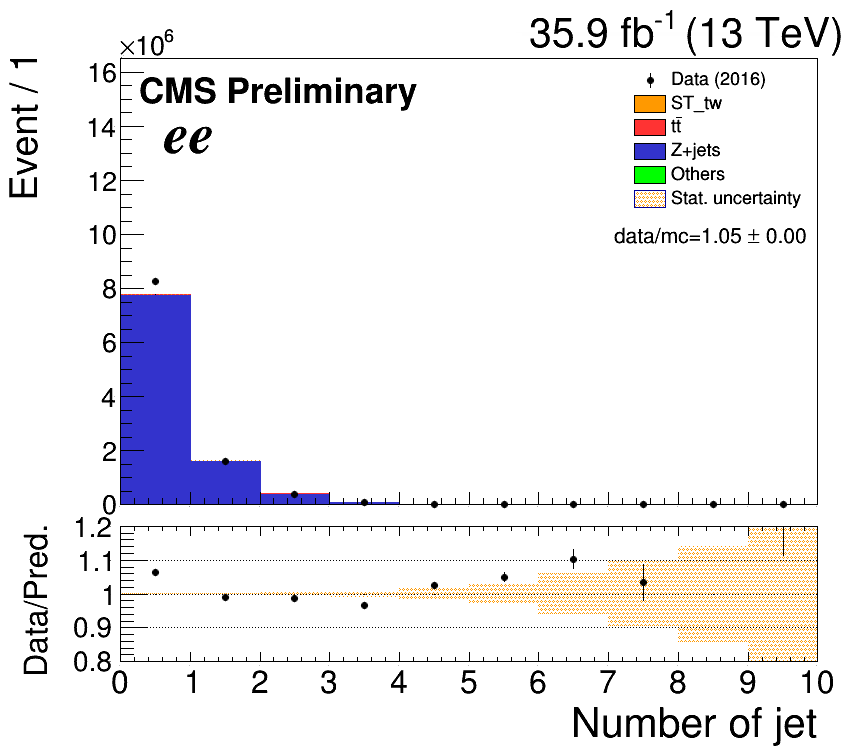
\includegraphics[width=0.32\textwidth]{figures/tW/fig/Step1/ee_noNvtx/H_N_loose_jets.png}&
%      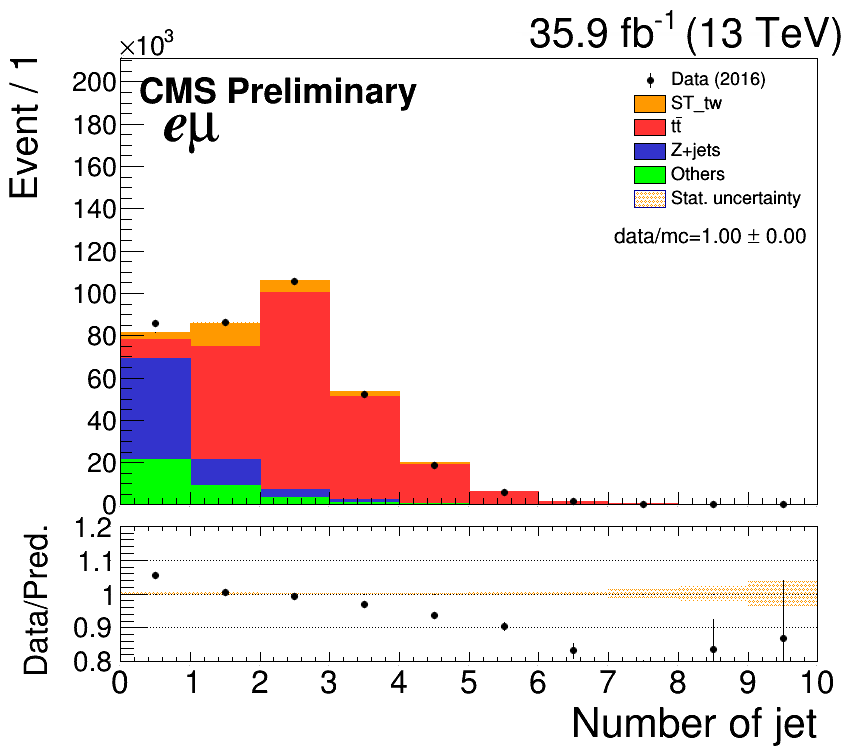
\includegraphics[width=0.32\textwidth]{figures/tW/fig/Step1/emu_noNvtx/H_N_loose_jets.png}&
%      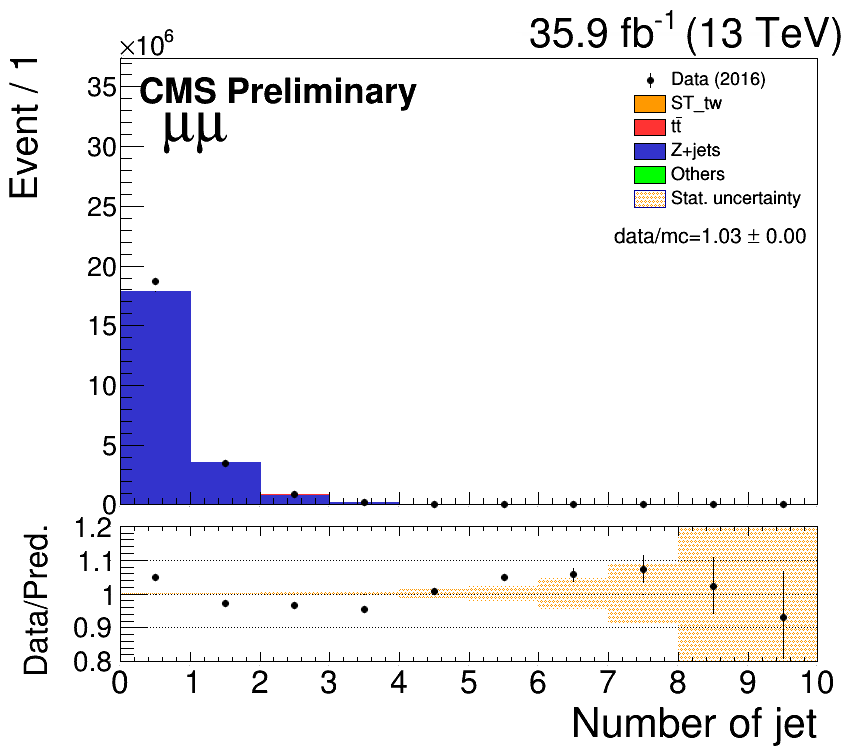
\includegraphics[width=0.32\textwidth]{figures/tW/fig/Step1/mumu_noNvtx/H_N_loose_jets.png}\\
%      \includegraphics[width=0.32\textwidth]{figures/tW/fig/Step1/ee_noNvtx/H_N_b_jets.png}&
%      \includegraphics[width=0.32\textwidth]{figures/tW/fig/Step1/emu_noNvtx/H_N_b_jets.png}&
%      \includegraphics[width=0.32\textwidth]{figures/tW/fig/Step1/mumu_noNvtx/H_N_b_jets.png}\\
%      \includegraphics[width=0.32\textwidth]{figures/tW/fig/Step1/ee_noNvtx/H_njet_bjet.png}&
%      \includegraphics[width=0.32\textwidth]{figures/tW/fig/Step1/emu_noNvtx/H_njet_bjet.png}&
%      \includegraphics[width=0.32\textwidth]{figures/tW/fig/Step1/mumu_noNvtx/H_njet_bjet.png}\\
%    \end{tabular}
%    \caption{The distributions of number of vertices (first row), number of jets (second row), number of b jets (third row) and number of jets-bjets (last row) for ee (left), $e\mu$ (middle) and \mumu (right) channels after step 1 (trigger and lepton selections). All backgrounds are estimated from MC.}
%    \label{fig:step1_Nvtx_jet_bjet}
%  \end{center}
%\end{figure}
%
%\begin{figure}[ht]
%  \begin{center}
%    \begin{tabular}{ccc}
%      \includegraphics[width=0.32\textwidth]{fig/EventSelection/_EE_80_step1_T2/EE_80_step1_T2_hratio_jet_leading_pt.png}&
%      \includegraphics[width=0.32\textwidth]{fig/EventSelection/_EMu_80_step1_T2/EMu_80_step1_T2_hratio_jet_leading_pt.png}&
%      \includegraphics[width=0.32\textwidth]{fig/EventSelection/_MuMu_80_step1_T2/MuMu_80_step1_T2_hratio_jet_leading_pt.png}\\
%      \includegraphics[width=0.32\textwidth]{fig/EventSelection/_EE_80_step1_T2/EE_80_step1_T2_hratio_jet_leading_eta.png}&
%      \includegraphics[width=0.32\textwidth]{fig/EventSelection/_EMu_80_step1_T2/EMu_80_step1_T2_hratio_jet_leading_eta.png}&
%      \includegraphics[width=0.32\textwidth]{fig/EventSelection/_MuMu_80_step1_T2/MuMu_80_step1_T2_hratio_jet_leading_eta.png}\\
%      \includegraphics[width=0.32\textwidth]{fig/EventSelection/_EE_80_step1_T2/EE_80_step1_T2_hratio_jet_leading_CSV.png}&
%      \includegraphics[width=0.32\textwidth]{fig/EventSelection/_EMu_80_step1_T2/EMu_80_step1_T2_hratio_jet_leading_CSV.png}&
%      \includegraphics[width=0.32\textwidth]{fig/EventSelection/_MuMu_80_step1_T2/MuMu_80_step1_T2_hratio_jet_leading_CSV.png}\\
%    \end{tabular}
%    \caption{The distributions of pt (first row), $\eta$ (second row) and csv discriminat (third row) of leading jet for ee (left), $e\mu$ (middle) and \mumu (right) channels after step 1 (trigger and lepton selections). All backgrounds are estimated from MC.}
%    \label{fig:step1_leading_jet_info}
%  \end{center}
%\end{figure}
%
%\begin{figure}[ht]
%  \begin{center}
%    \begin{tabular}{ccc}
%      \includegraphics[width=0.32\textwidth]{fig/EventSelection/_EE_80_step1_T2/EE_80_step1_T2_hratio_jet_sub_leading_pt.png}&
%      \includegraphics[width=0.32\textwidth]{fig/EventSelection/_EMu_80_step1_T2/EMu_80_step1_T2_hratio_jet_sub_leading_pt.png}&
%      \includegraphics[width=0.32\textwidth]{fig/EventSelection/_MuMu_80_step1_T2/MuMu_80_step1_T2_hratio_jet_sub_leading_pt.png}\\
%      \includegraphics[width=0.32\textwidth]{fig/EventSelection/_EE_80_step1_T2/EE_80_step1_T2_hratio_jet_sub_leading_eta.png}&
%      \includegraphics[width=0.32\textwidth]{fig/EventSelection/_EMu_80_step1_T2/EMu_80_step1_T2_hratio_jet_sub_leading_eta.png}&
%      \includegraphics[width=0.32\textwidth]{fig/EventSelection/_MuMu_80_step1_T2/MuMu_80_step1_T2_hratio_jet_sub_leading_eta.png}\\
%      \includegraphics[width=0.32\textwidth]{fig/EventSelection/_EE_80_step1_T2/EE_80_step1_T2_hratio_jet_sub_leading_CSV.png}&
%      \includegraphics[width=0.32\textwidth]{fig/EventSelection/_EMu_80_step1_T2/EMu_80_step1_T2_hratio_jet_sub_leading_CSV.png}&
%      \includegraphics[width=0.32\textwidth]{fig/EventSelection/_MuMu_80_step1_T2/MuMu_80_step1_T2_hratio_jet_sub_leading_CSV.png}\\
%    \end{tabular}
%    \caption{The distributions of pt (first row), $\eta$ (second row) and csv discriminat (third row) of sub-leading jet for ee (left), $e\mu$ (middle) and \mumu (right) channels after step 1 (trigger and lepton selections). All backgrounds are estimated from MC.}
%    \label{fig:step1_subleading_jet_info}
%  \end{center}
%\end{figure}

\clearpage
\section{Background Predictions}
\label{tW_background}

\subsection{Prompt Background}
\label{tW_DY_background}
The background from processes giving two prompt leptons is taken from MC samples and normalized to the luminosity. It consists mostly of events from \ttbar production, Drell-Yan, and WW productions. Other background processes considered are the other diboson processes like WZ and ZZ.

In the \mumu and ee final states, the normalization of the DY background simulation is estimated from data using the method described in~\cite{topPAS11_002,TOP-11-005_paper,TOP-12-007_paper,bib:TOP-15-003_paper}, extracting the events outside the Z-veto region from the events inside.
As described above, events in this region have a dilepton invariant mass between 76 GeV and 106 GeV and are rejected for the analysis.
Since contamination from non-DY background contributions can still be present in the Z-veto region, this contribution is subtracted from the e$\mu$ channel and then scaled according to the event yields in the ee and \mumu channels.

The expected number of events outside the Z-veto can be measured from data as:
%\begin{eqnarray}
$$N^{ll, Z+jets~data}_{out} = R^{ll}_{out/in}( N^{ll,data}_{in} -0.5 N^{e\mu,data}_{in} k_{ll})$$
%\label{eq:dyest}
%\end{eqnarray}
where $ll = \mu\mu$  or ee  and $R_{out/in}$ is the ratio of the number of events outside/inside the Z-veto region taken from the DY simulated sample:
$$R_{out/in}= \frac{N^{ll,Z+jets~MC}_{out}}{N^{ll,Z+jets~MC}_{in}}.$$

Here, $k_{ll}$ is a correction factor that takes into account the differences between electron and muon reconstruction.
This correction can be determined from the number of ee and \mumu events in the Z peak region after applying the MET requirement (labeled as \textit{loose}).
Since $N^{ee_{in, loose}}$ and $N^{\mumu_{in, loose}}$ are proportional to the square of the corresponding single-lepton candidate selection efficiencies, the correction factor can be expressed as: $$k_{ee} = \sqrt{\frac{N^{ee_{in, loose}}}{N^{\mumu_{in, loose}}}}$$
$$k_{\mu\mu} = \sqrt{\frac{N^{\mumu_{in, loose}}}{N^{ee_{in, loose}}}}$$

The values of $k_{ll}$ for different njet-nbjet regions are shown in Table \ref{tab:kll}. We use explicitly $k_{ll}$ for different njet-nbjet regions.
\begin{table}[ht]
\centering
\begin{tabular}{|c|c|c|c|c|}
\hline
Channel                                 & all                                       & 1jet,1tag                 & 2jet,1tag             & \textgreater=2jet,2tag \\ \hline
$N^{ee_{in, loose}}$ (data)             & 220435                                    & 3805                      & 3735                  & 2493                   \\ \hline
$N^{\mu\mu_{in, loose}}$ (data)         & 501781                                    & 8291                      & 7550                  & 5180                  \\ \hline
$k_{ee}$                                & 0.66 $\pm$ 0.001                          & 0.68 $\pm$ 0.007          & 0.70 $\pm$ 0.007      & 0.69 $\pm$ 0.008         \\ \hline
$k_{\mu\mu}$                            & 1.51 $\pm$ 0.002                          & 1.48 $\pm$ 0.014          & 1.42 $\pm$ 0.014      & 1.44 $\pm$ 0.018         \\ \hline
\end{tabular}
\caption{The values of $k_{ll}$ for different njet-nbjet regions. Errors are statistical uncertainties only.}
\label{tab:kll}
\end{table}




The global scaling factors $${C}_{Z+jets}=\frac{N^{ll, Z+jets~data}_{out}}{N^{ll,Z+jets~MC}_{out}}$$ are determined.
The results and scaling factors are summarized in Table~\ref{tab:DY_scale}.


\begin{table}[h]
\centering
\begin{tabular}{|c|c|c|c|c|c|c|c|c|}
\hline
                                   & \multicolumn{2}{c|}{All} & \multicolumn{2}{c|}{1jet,1tag} & \multicolumn{2}{c|}{2jet,1tag} & \multicolumn{2}{c|}{$>=2jet,2tag$} \\ \hline
                                   & ee       & \mumu    & ee         & \mumu        & ee         & \mumu        & ee           & \mumu          \\ \hline
$N^{ll,Z+jets~MC}_{in} $           & 243878.3   & 562506.9    & 2712.3       & 6490.7          & 1550.6       & 3734.2          & 306.8          & 712.7             \\ \hline
$N^{ll,Z+jets~MC}_{out}$           & 22376      & 56494.6     & 301.4        & 878.7           & 280.8        & 590.9           & 53.7           & 94.1              \\ \hline
$R_{out/in}$                       & 0.092      & 0.100       & 0.111        & 0.135           & 0.181        & 0.158           & 0.175          & 0.132             \\ \hline
$N^{ll,data}_{in}$                 & 220435     & 501781      & 3805         & 8291            & 3735         & 7550            & 2493           & 5180              \\ \hline
$N^{e\mu,data}_{in}$               & 34322      & 34322       & 4453         & 4453            & 6230         & 6230            & 6259           & 6259              \\ \hline
$N^{ll,Z+jets~data}_{out}$         & 19185.9    & 47793.1     & 254.6        & 676.3           & 281.6        & 494.8           & 58.4           & 89.0              \\ \hline
$C_{Z+jets}$                       & 0.857      & 0.846       & 0.845        & 0.770           & 1.002        & 0.837           & 1.087          & 0.945             \\
                                   & $\pm$ 0.004& $\pm$ 0.003 & $\pm$ 0.049  & $\pm$ 0.030     & $\pm$ 0.085  & $\pm$ 0.048     & $\pm$ 0.28    & $\pm$ 0.181 \\ \hline
\end{tabular}
\caption{Data-driven Z$+$jets background estimation in the \mumu and ee
channels after the ``$Step1+Step2$'' selection requirements. Errors are statistical uncertainties only.}
\label{tab:DY_scale}
\end{table}




\subsection{Fake Background}
\label{tW_fake_background}

%In e$mu$ final state, the background from DY events decaying to dimuons or dielectrons where one of the two leptons is then
%misidentified as the other lepton flavour is taken from MC events normalized to the luminosity.
Another source of events with misidentified leptons is the W$\gamma$ process,
where the W decays to an electron and a neutrino and the photon is either misidentified as electron, or the photon converts and gives an electron. This background contribution is taken from MC simulation. For the backgrounds which involve a jet that are misidentified as an electron or muon, a data-driven technique is used.

The jet background (or called Nonprompt background) consists of events where a jet is reconstructed as an electron or muon that
passes the selection, coming mostly from W+jets process and QCD.
The method which is used to estimate the jet background is called same sign
method. In the same sign method, we use the fact that the probability of assigning positive or
negative charge to the misidentified jet should be equal. Therefore, opposite and same-sign  pairs are similar for fake jets in total number and distribution shape for many variables.
On the other hand, all other standard model processes have opposite sign electron pairs and
do not contribute to the same sign control region. The contributions of the prompt backgrounds
are subtracted from data in the same sign region using MC samples  to find the jets contribution in the opposite sign region (signal region).

%Figure \ref{fig:ss_bkg} shows a comparison between data and MC
%in same sign control region. Missed MC backgrounds are $W$+jets and QCD. In Table \ref{tab:samesign} the number of events for data and MC backgrounds are shown.
%In Table \ref{tab:samesign}, number of data events and prompt background events in the same sign region are written.
%In Table \ref{faketab}, number of  expected  QCD events in various channel and njet-mtag regions using same sign methods are written.
%All Backgrounds except \ttbar, $tW$, DY and jets are combined and shown as 'other' in all plots.
%
%\begin{table}[]
%\centering
%\caption{Number of events in the same-sign region}
%\label{tab:samesign}
%\begin{tabular}{|c|c|c|c|c|c|}
%\hline
%                          &           & 1jet,0tag& 1jet,1tag & 2jet,1tag & $>=$2jet,2tag \\ \hline
%\multirow{5}{*}{ee}     & data      & -        & 112       &  137      &  132    \\ \cline{2-6}
%                          & tW        & -        & 11        &  8        &  4      \\ \cline{2-6}
%                          & $t\bar{t}$& -        & 75        &  99       &  88     \\ \cline{2-6}
%                          & DY        & -        & 15        &  2        &  2      \\ \cline{2-6}
%                          & other     & -        & 11        &  12       &  19     \\ \hline
%\multirow{5}{*}{$e\mu$}   & data      & 4057     & 742       &  882      &  579    \\ \cline{2-6}
%                          & tW        & 69       & 40        &  31       &  12     \\ \cline{2-6}
%                          & $t\bar{t}$& 282      & 307       &  365      &  268    \\ \cline{2-6}
%                          & DY        & 638      & 31        &  20       &  0      \\ \cline{2-6}
%                          & other     & 1657     & 68        &  76       &  73     \\ \hline
%\multirow{5}{*}{\mumu} & data      & -        & 154       &  205      &  63     \\ \cline{2-6}
%                          & tW        & -        & 3         &  5        &  1      \\ \cline{2-6}
%                          & $t\bar{t}$& -        & 57        &  48       &  7      \\ \cline{2-6}
%                          & DY        & -        & 0         &  3        &  0      \\ \cline{2-6}
%                          & other     & -        & 8         &  17       &  23     \\ \hline
%\end{tabular}
%\end{table}
%
%\begin{table}[h]
%\centering
%\caption{Number of  expected  events from jets bacgrounds in various channels and njet-mtag regions using the same sign methods. These numbers are data events in the same sign region minus the contribution of prompt BG using MC prediction.}
%\label{faketab}
%\begin{tabular}{|l|l|l|l|}
%\hline
%                & ee & \mumu & $e\mu$ \\ \hline
%$1jet,0tag$     & -    & -        & 1411   \\ \hline
%$1jet,1tag$     & 0    & 87       & 296    \\ \hline
%$2jet,1tag$     & 15   & 133      & 390    \\ \hline
%$>=2jet, 2tag $ & 19   & 32       & 225    \\ \hline
%\end{tabular}
%\end{table}
%
%\begin{figure}[ht]
%  \begin{center}
%    \begin{tabular}{ccc}
%      \includegraphics[width=0.32\textwidth]{fig/ss_bkg/_SS_EMu_80_step1_T2_1j0b_ss/EMu_80_step1_T2_1j0b_ss_hratio_new_M_ll.png}&
%      \includegraphics[width=0.32\textwidth]{fig/ss_bkg/_SS_EMu_80_step1_T2_1j0b_ss/EMu_80_step1_T2_1j0b_ss_hratio_new_leading_pt.png}&
%      \includegraphics[width=0.32\textwidth]{fig/ss_bkg/_SS_EMu_80_step1_T2_1j0b_ss/EMu_80_step1_T2_1j0b_ss_hratio_new_sub_leading_pt.png}\\
%      \includegraphics[width=0.32\textwidth]{fig/ss_bkg/_SS_EMu_80_step1_T2_1j0b_ss/EMu_80_step1_T2_1j0b_ss_hratio_MET_pt.png}&
%      \includegraphics[width=0.32\textwidth]{fig/ss_bkg/_SS_EMu_80_step1_T2_1j0b_ss/EMu_80_step1_T2_1j0b_ss_hratio_MET_phi.png}&
%      \includegraphics[width=0.32\textwidth]{fig/ss_bkg/_SS_EMu_80_step1_T2_1j0b_ss/EMu_80_step1_T2_1j0b_ss_hratio_leading_eta.png}\\
%      \includegraphics[width=0.32\textwidth]{fig/ss_bkg/_SS_EMu_80_step1_T2_1j0b_ss/EMu_80_step1_T2_1j0b_ss_hratio_leading_phi.png}&
%      \includegraphics[width=0.32\textwidth]{fig/ss_bkg/_SS_EMu_80_step1_T2_1j0b_ss/EMu_80_step1_T2_1j0b_ss_hratio_Pt_ll.png}&
%      \includegraphics[width=0.32\textwidth]{fig/ss_bkg/_SS_EMu_80_step1_T2_1j0b_ss/EMu_80_step1_T2_1j0b_ss_hratio_phi_ll.png}\\
%      \includegraphics[width=0.32\textwidth]{fig/ss_bkg/_SS_EMu_80_step1_T2_1j0b_ss/EMu_80_step1_T2_1j0b_ss_hratio_MVA_MLP.png}&
%      \includegraphics[width=0.32\textwidth]{fig/ss_bkg/_SS_EMu_80_step1_T2_1j0b_ss/EMu_80_step1_T2_1j0b_ss_hratio_phi_ll.png}&
%      \includegraphics[width=0.32\textwidth]{fig/ss_bkg/_SS_EMu_80_step1_T2_1j0b_ss/EMu_80_step1_T2_1j0b_ss_hratio_pv_n.png}\\
%    \end{tabular}
%    \caption{The same sign distributions of some variables in $e\mu$ [1 jet, 0 tag] region.}
%    \label{fig:ss_bkg}
%  \end{center}
%\end{figure}

\clearpage
\section{Data/MC Comparison}
\label{tW_data_mc}
After all selections and background estimation, the expected numbers of events from tW, t$\bar{\rm t}$, DY and remaining background contributions mentioned above, as well as the total number of background events are reported in Table~\ref{tab:total_event} for the ee and \mumu channels and for the various (n-jets,m-tags) categories. The data and MC comparison are shown in Figures \ref{fig:step2_leading_lepton}-\ref{fig:step2_MET_phi_Dphi_DR}. The definitions of $\mathrm{HT^{syst}}$, $\mathrm{\pt^{syst}}$, and $\mathrm{MT^{syst}}$ in Figure \ref{fig:step2_HT_Pt_Mt_rho} are $\mathrm{HT^{syst}=\sum{\pt^{jet}}+\sum{\pt^{lepton}}}$, $\mathrm{\pt^{syst}=\sum{\overrightarrow{\pt^{jet}}}+\sum{\overrightarrow{\pt^{lepton}}}}$, $\mathrm{MT^{syst}=\sqrt{(HT^{syst})^{2}-(\pt^{syst})^{2}}}$.
In Figure \ref{fig:binee}, the data in the six (three ee plus three \mumu) search regions are shown together with the predictions for the SM backgrounds. The sources of systematic uncertainties which are considered in the Table \ref{tab:total_event} and the plots of Figures \ref{fig:step2_leading_lepton}-\ref{fig:binee} are explained in Section \ref{tW_systematic}.

\begin{table}[h]
\centering
\resizebox{\linewidth}{!}{
\begin{tabular}{|c|c|c|c|c|c|c|c|}
\hline
\multirow{2}{*}{Channel}  & \multirow{2}{*}{(n-jets,m-tags)}  & \multicolumn{5}{c|}{Prediction}   & \multirow{2}{*}{Data}     \\ \cline{3-7}
                          &                                        & tW                 & t$\bar{\rm t}$     & DY                   & Other + nonprompt        &  Total predicted yield   &        \\ \hline
\multirow{3}{*}{ee}       & (1,1)     & 884$\pm$8    &4741$\pm$15 &258$\pm$50   & 53$\pm$5     &5936$\pm$470   & 5902$\pm$76   \\ \cline{2-8}
                          & (2,1)     & 518$\pm$6    &7479$\pm$19 &241$\pm$53   & 94$\pm$5     &8331$\pm$597   & 8266$\pm$90   \\ \cline{2-8}
                          & ($\ge$2,2)& 267$\pm$4    &7561$\pm$18 &46$\pm$24    & 99$\pm$4     &7973$\pm$819   & 7945$\pm$89   \\ \hline
%\multirow{4}{*}{e$\upmu$}   & (1,0)     & 4835$\pm$20  &23557$\pm$35&11352$\pm$277& 10294$\pm$72 &50038$\pm$6931 & 48973$\pm$221     \\ \cline{2-8}
%                          & (1,1)     & 6048$\pm$22  &30436$\pm$38&561$\pm$66   & 629$\pm$13   &37673$\pm$2984 & 37370$\pm$193     \\ \cline{2-8}
%                          & (2,1)     & 3117$\pm$16  &47206$\pm$48&278$\pm$48  & 781$\pm$9    &51382$\pm$3714  & 50725$\pm$225    \\ \cline{2-8}
%                          & ($\ge$2,2)& 1450$\pm$10  &47310$\pm$46&32$\pm$22    & 598$\pm$9    &49391$\pm$5010 & 49262$\pm$221    \\ \hline
\multirow{3}{*}{\mumu} & (1,1)     & 1738$\pm$12  &9700$\pm$21 &744$\pm$90  & 183$\pm$5    &12366$\pm$879   & 12178$\pm$110  \\ \cline{2-8}
                          & (2,1)     & 989$\pm$9    &14987$\pm$27&501$\pm$75   & 275$\pm$5    &16751$\pm$1276 & 16395$\pm$128  \\ \cline{2-8}
                          & ($\ge$2,2)& 508$\pm$6    &15136$\pm$26&82$\pm$24    & 163$\pm$5  &15889$\pm$1714   & 15838$\pm$125 \\ \hline
\end{tabular}}
\caption{Numbers of expected events from tW, t$\bar{\rm t}$, and DY productions, from the remaining  backgrounds (other and nonprompt backgrounds), total background contribution and observed events in data after all selections for the ee and \mumu channels and for various (n-jets,m-tags) categories.
The uncertainties correspond to the statistical contribution only for the individual background predictions and to the quadratic sum of the statistical and systematic contributions for the total background predictions.}
\label{tab:total_event}
\end{table}



%\begin{table}[ht]
%\centering
%\begin{tabular}{|c|c|c||c|c|}
%\hline
%Channel & ee               & fraction & \mumu       & fraction  \\ \hline
%tW      & 3674  +/- 26       & 5.62\%   & 7103   +/- 24  & 5.08\%  \\ \hline
%TTbar   & 38209 +/- 62       & 58.41\%  & 75949  +/- 61  & 54.37\% \\ \hline
%DY      & 19176 +/- 5749     & 29.31\%  & 47845  +/- 627 & 34.25\% \\ \hline
%WW      & 2687  +/- 47       & 4.11\%   & 5638   +/- 39  & 4.04\%  \\ \hline
%WG      & 344   +/- 75       & 0.53\%   & 46     +/- 17  & 0.03\%  \\ \hline
%WZ      & 400   +/- 23       & 0.61\%   & 762    +/- 8   & 0.55\%  \\ \hline
%TTG     & 232   +/- 10       & 0.35\%   & 407    +/- 10  & 0.29\%  \\ \hline
%ZZ      & 86    +/- 3        & 0.13\%   & 184    +/- 1   & 0.13\%  \\ \hline
%HWW     & 261   +/- 11       & 0.40\%   & 586    +/- 10  & 0.42\%  \\ \hline
%TTWJets & 21    +/- 4        & 0.03\%   & 38     +/- 4   & 0.03\%  \\ \hline
%Jets     & 428   +/- 75       & 0.50\%   & 1356   +/- 54  & 0.82\%  \\ \hline \hline
%data    & 64474 +/- 254      &          & 137094 +/- 370 &         \\ \hline
%Pred    & 65518 +/- 5750     &          & 139914 +/- 632 &         \\ \hline
%
%\hline
%\hline
%Channel & $e\mu$         & fraction  & $Combined$      & fraction \\ \hline
%tW      & 23057  +/- 43  & 6.43\%    & 33834  +/- 56   & 6.00\%  \\ \hline
%TTbar   & 232161 +/- 106 & 64.71\%   & 346319 +/- 138  & 61.42\% \\ \hline
%DY      & 64880  +/- 559 & 18.08\%   & 131901 +/- 5810 & 23.39\% \\ \hline
%WW      & 25864  +/- 82  & 7.21\%    & 34188  +/- 102  & 6.06\%  \\ \hline
%WG      & 1958   +/- 95  & 0.55\%    & 2348   +/- 122  & 0.42\%  \\ \hline
%WZ      & 2369   +/- 14  & 0.66\%    & 3531   +/- 28   & 0.63\%  \\ \hline
%TTG     & 1115   +/- 16  & 0.31\%    & 1754   +/- 21   & 0.31\%  \\ \hline
%ZZ      & 484    +/- 2   & 0.13\%    & 753    +/- 4    & 0.13\%  \\ \hline
%HWW     & 2430   +/- 20  & 0.68\%    & 3277   +/- 25   & 0.58\%  \\ \hline
%TTWJets & 121    +/- 7   & 0.03\%    & 180    +/- 9    & 0.03\%  \\ \hline
%Jets     & 4318   +/- 447 & 1.20\%    & 9256   +/- 248  & 1.03\%  \\ \hline \hline
%data    & 356383 +/- 597 &           & 557951 +/- 747  &         \\ \hline
%Pred    & 361909 +/- 585 &           & 567341 +/- 5814 &         \\ \hline
%\end{tabular}
%\caption{Cut flow Table after step2 (full selection). The contribution from jets and DY normalization k-factors are  estimated from data and  errors are MC statistical uncertainties only.}
%\label{tab:cut_flow_step2}
%\end{table}




\begin{figure}[ht]
  \begin{center}
    \begin{tabular}{ccc}
      \includegraphics[width=0.4\textwidth]{figures/tW/fig/Step2/ee/H_lepton_led_pt.png}&
      \includegraphics[width=0.4\textwidth]{figures/tW/fig/Step2/mumu/H_lepton_led_pt.png}\\
      \includegraphics[width=0.4\textwidth]{figures/tW/fig/Step2/ee/H_lepton_led_eta.png}&
      \includegraphics[width=0.4\textwidth]{figures/tW/fig/Step2/mumu/H_lepton_led_eta.png}\\
      \includegraphics[width=0.4\textwidth]{figures/tW/fig/Step2/ee/H_lepton_led_phi.png}&
      \includegraphics[width=0.4\textwidth]{figures/tW/fig/Step2/mumu/H_lepton_led_phi.png}\\
    \end{tabular}
    \caption{The distributions of \pt (top), $\eta$ (middle) and $\phi$ (bottom) of leading lepton for ee (left) and \mumu (right) channels after step 2 (full selection).
    \label{fig:step2_leading_lepton}}
  \end{center}
\end{figure}

\begin{figure}[ht]
  \begin{center}
    \begin{tabular}{ccc}
      \includegraphics[width=0.4\textwidth]{figures/tW/fig/Step2/ee/H_lepton_sub_pt.png}&
      \includegraphics[width=0.4\textwidth]{figures/tW/fig/Step2/mumu/H_lepton_sub_pt.png}\\
      \includegraphics[width=0.4\textwidth]{figures/tW/fig/Step2/ee/H_lepton_sub_eta.png}&
      \includegraphics[width=0.4\textwidth]{figures/tW/fig/Step2/mumu/H_lepton_sub_eta.png}\\
      \includegraphics[width=0.4\textwidth]{figures/tW/fig/Step2/ee/H_lepton_sub_phi.png}&
      \includegraphics[width=0.4\textwidth]{figures/tW/fig/Step2/mumu/H_lepton_sub_phi.png}\\
    \end{tabular}
    \caption{The distributions of \pt (top), $\eta$ (middle) and $\phi$ (bottom) of sub-leading lepton for ee (left) and \mumu (right) channels after step 2 (full selection).
    \label{fig:step2_subleading_lepton}}
  \end{center}
\end{figure}


\begin{figure}[ht]
  \begin{center}
    \begin{tabular}{ccc}
      \includegraphics[width=0.4\textwidth]{figures/tW/fig/Step2/ee/H_Mll.png}&
      \includegraphics[width=0.4\textwidth]{figures/tW/fig/Step2/mumu/H_Mll.png}\\
      \includegraphics[width=0.4\textwidth]{figures/tW/fig/Step2/ee/H_Ptll.png}&
      \includegraphics[width=0.4\textwidth]{figures/tW/fig/Step2/mumu/H_Ptll.png}\\
      \includegraphics[width=0.4\textwidth]{figures/tW/fig/Step2/ee/H_Rll.png}&
      \includegraphics[width=0.4\textwidth]{figures/tW/fig/Step2/mumu/H_Rll.png}\\
      \includegraphics[width=0.4\textwidth]{figures/tW/fig/Step2/ee/H_Ptll_phi.png}&
      \includegraphics[width=0.4\textwidth]{figures/tW/fig/Step2/mumu/H_Ptll_phi.png}\\
    \end{tabular}
    \caption{The distributions of invariant mass of two leptons (first row), \pt of two leptons (second row), Rapidity of two leptons (third row) and $\phi$ of two leptons (last row) for ee (left) and \mumu (right) channels after step 2 (full selection).
    \label{fig:step2_M_pt_R_phi}}
  \end{center}
\end{figure}


\begin{figure}[ht]
  \begin{center}
    \begin{tabular}{ccc}
      \includegraphics[width=0.4\textwidth]{figures/tW/fig/Step2/ee/H_pv_n.png}&
      \includegraphics[width=0.4\textwidth]{figures/tW/fig/Step2/mumu/H_pv_n.png}\\
      \includegraphics[width=0.4\textwidth]{figures/tW/fig/Step2/ee/H_N_loose_jets.png}&
      \includegraphics[width=0.4\textwidth]{figures/tW/fig/Step2/mumu/H_N_loose_jets.png}\\
      \includegraphics[width=0.4\textwidth]{figures/tW/fig/Step2/ee/H_N_b_jets.png}&
      \includegraphics[width=0.4\textwidth]{figures/tW/fig/Step2/mumu/H_N_b_jets.png}\\
      \includegraphics[width=0.4\textwidth]{figures/tW/fig/Step2/ee/H_njet_bjet.png}&
      \includegraphics[width=0.4\textwidth]{figures/tW/fig/Step2/mumu/H_njet_bjet.png}\\
    \end{tabular}
    \caption{The distributions of number of vertices (first row), number of jet (second row), number of b jets (third row) and number of jet-bjets (last row) for ee (left) and \mumu (right) channels after step 2 (full selection).
    \label{fig:step2_Nvtx_jet_bjet}}
  \end{center}
\end{figure}


\begin{figure}[ht]
  \begin{center}
    \begin{tabular}{ccc}
      \includegraphics[width=0.4\textwidth]{figures/tW/fig/Step2/ee/H_HT_sys.png}   &
      \includegraphics[width=0.4\textwidth]{figures/tW/fig/Step2/mumu/H_HT_sys.png} \\
      \includegraphics[width=0.4\textwidth]{figures/tW/fig/Step2/ee/H_Pt_sys.png}   &
      \includegraphics[width=0.4\textwidth]{figures/tW/fig/Step2/mumu/H_Pt_sys.png} \\
      \includegraphics[width=0.4\textwidth]{figures/tW/fig/Step2/ee/H_MT_sys.png}    &
      \includegraphics[width=0.4\textwidth]{figures/tW/fig/Step2/mumu/H_MT_sys.png}  \\
      \includegraphics[width=0.4\textwidth]{figures/tW/fig/Step2/ee/H_rho.png}&
      \includegraphics[width=0.4\textwidth]{figures/tW/fig/Step2/mumu/H_rho.png}\\
    \end{tabular}
    \caption{The distributions of $\mathrm{HT^{syst}}$ (first row), $\mathrm{\pt^{syst}}$ (second row), $\mathrm{MT^{syst}}$ (third row)  and $\rho$ for ee (left) and \mumu (right) channels after step 2 (full selection).
    \label{fig:step2_HT_Pt_Mt_rho}}
  \end{center}
\end{figure}




\begin{figure}[ht]
  \begin{center}
    \begin{tabular}{ccc}
      \includegraphics[width=0.4\textwidth]{figures/tW/fig/Step2/ee/H_MET_Et.png}&
      \includegraphics[width=0.4\textwidth]{figures/tW/fig/Step2/mumu/H_MET_Et.png}\\
%      \includegraphics[width=0.4\textwidth]{figures/tW/fig/Step2/ee/H_MET_phi.png}&
%      \includegraphics[width=0.4\textwidth]{figures/tW/fig/Step2/mumu/H_MET_phi.png}\\
      \includegraphics[width=0.4\textwidth]{figures/tW/fig/Step2/ee/H_ll_Dphi.png}&
      \includegraphics[width=0.4\textwidth]{figures/tW/fig/Step2/mumu/H_ll_Dphi.png}\\
      \includegraphics[width=0.4\textwidth]{figures/tW/fig/Step2/ee/H_ll_DR.png}&
      \includegraphics[width=0.4\textwidth]{figures/tW/fig/Step2/mumu/H_ll_DR.png}\\
    \end{tabular}
    \caption{The distributions of MET (top row), $\Delta\phi$ between two leptons (middle row) and $\Delta R$ between two leptons (bottom row) for ee (left) and \mumu (right) channels after step 2 (full selection).
    \label{fig:step2_MET_phi_Dphi_DR}}
  \end{center}
\end{figure}

\begin{figure}[ht]
  \begin{center}
    \begin{tabular}{cc}
      \includegraphics[width=0.45\textwidth]{figures/tW/fig/Result/ee/H_Limit_N_jet_bjet.png}&
      \includegraphics[width=0.45\textwidth]{figures/tW/fig/Result/mumu/H_Limit_N_jet_bjet.png}\\
    \end{tabular}
    \caption{The observed numbers of events and SM background predictions in the search regions of the analysis for the ee (left), \mumu (right) channels. The hatched band corresponds to the quadratic sum of statistical and systematic uncertainties in the event yield for the SM background predictions. The ratios of data to the sum of the predicted yields are shown at the bottom of each plot. The narrow hatched band represents the contribution from the statistical uncertainty in the MC simulation.
    \label{fig:binee}}
  \end{center}
\end{figure}



\clearpage







%\begin{figure}[ht]
%  \begin{center}
%    \begin{tabular}{ccc}
%      \includegraphics[width=0.32\textwidth]{figures/tW/fig/Step2/ee/H_lepton_led_pt.png}&
%      \includegraphics[width=0.32\textwidth]{figures/tW/fig/Step2/emu/H_lepton_led_pt.png}&
%      \includegraphics[width=0.32\textwidth]{figures/tW/fig/Step2/mumu/H_lepton_led_pt.png}\\
%      \includegraphics[width=0.32\textwidth]{figures/tW/fig/Step2/ee/H_lepton_led_eta.png}&
%      \includegraphics[width=0.32\textwidth]{figures/tW/fig/Step2/emu/H_lepton_led_eta.png}&
%      \includegraphics[width=0.32\textwidth]{figures/tW/fig/Step2/mumu/H_lepton_led_eta.png}\\
%      \includegraphics[width=0.32\textwidth]{figures/tW/fig/Step2/ee/H_lepton_led_phi.png}&
%      \includegraphics[width=0.32\textwidth]{figures/tW/fig/Step2/emu/H_lepton_led_phi.png}&
%      \includegraphics[width=0.32\textwidth]{figures/tW/fig/Step2/mumu/H_lepton_led_phi.png}\\
%    \end{tabular}
%    \caption{The distributions of Pt (top), $\eta$ (middle) and $\phi$ (bottom) of leading lepton for ee (left), $e\mu$ (middle) and \mumu (right) channels after step 2 (full selection).
%    \label{fig:step2_leading_lepton}}
%  \end{center}
%\end{figure}
%
%\begin{figure}[ht]
%  \begin{center}
%    \begin{tabular}{ccc}
%      \includegraphics[width=0.32\textwidth]{figures/tW/fig/Step2/ee/H_lepton_sub_pt.png}&
%      \includegraphics[width=0.32\textwidth]{figures/tW/fig/Step2/emu/H_lepton_sub_pt.png}&
%      \includegraphics[width=0.32\textwidth]{figures/tW/fig/Step2/mumu/H_lepton_sub_pt.png}\\
%      \includegraphics[width=0.32\textwidth]{figures/tW/fig/Step2/ee/H_lepton_sub_eta.png}&
%      \includegraphics[width=0.32\textwidth]{figures/tW/fig/Step2/emu/H_lepton_sub_eta.png}&
%      \includegraphics[width=0.32\textwidth]{figures/tW/fig/Step2/mumu/H_lepton_sub_eta.png}\\
%      \includegraphics[width=0.32\textwidth]{figures/tW/fig/Step2/ee/H_lepton_sub_phi.png}&
%      \includegraphics[width=0.32\textwidth]{figures/tW/fig/Step2/emu/H_lepton_sub_phi.png}&
%      \includegraphics[width=0.32\textwidth]{figures/tW/fig/Step2/mumu/H_lepton_sub_phi.png}\\
%    \end{tabular}
%    \caption{The distributions of Pt (top), $\eta$ (middle) and $\phi$ (bottom) of sub-leading lepton for ee (left), $e\mu$ (middle) and \mumu (right) channels after step 2 (full selection).
%    \label{fig:step2_subleading_lepton}}
%  \end{center}
%\end{figure}
%
%
%\begin{figure}[ht]
%  \begin{center}
%    \begin{tabular}{ccc}
%      \includegraphics[width=0.32\textwidth]{figures/tW/fig/Step2/ee/H_Mll.png}&
%      \includegraphics[width=0.32\textwidth]{figures/tW/fig/Step2/emu/H_Mll.png}&
%      \includegraphics[width=0.32\textwidth]{figures/tW/fig/Step2/mumu/H_Mll.png}\\
%      \includegraphics[width=0.32\textwidth]{figures/tW/fig/Step2/ee/H_Ptll.png}&
%      \includegraphics[width=0.32\textwidth]{figures/tW/fig/Step2/emu/H_Ptll.png}&
%      \includegraphics[width=0.32\textwidth]{figures/tW/fig/Step2/mumu/H_Ptll.png}\\
%      \includegraphics[width=0.32\textwidth]{figures/tW/fig/Step2/ee/H_Rll.png}&
%      \includegraphics[width=0.32\textwidth]{figures/tW/fig/Step2/emu/H_Rll.png}&
%      \includegraphics[width=0.32\textwidth]{figures/tW/fig/Step2/mumu/H_Rll.png}\\
%      \includegraphics[width=0.32\textwidth]{figures/tW/fig/Step2/ee/H_Ptll_phi.png}&
%      \includegraphics[width=0.32\textwidth]{figures/tW/fig/Step2/emu/H_Ptll_phi.png}&
%      \includegraphics[width=0.32\textwidth]{figures/tW/fig/Step2/mumu/H_Ptll_phi.png}\\
%    \end{tabular}
%    \caption{The distributions of invariant mass of two leptons (first row), Pt of two leptons (second row), Rapidity of two leptons (third row) and $\phi$ of two leptons (last row) for ee (left), $e\mu$ (middle) and \mumu (right) channels after step 2 (full selection).
%    \label{fig:step2_M_pt_R_phi}}
%  \end{center}
%\end{figure}
%
%
%\begin{figure}[ht]
%  \begin{center}
%    \begin{tabular}{ccc}
%      \includegraphics[width=0.32\textwidth]{figures/tW/fig/Step2/ee/H_pv_n.png}&
%      \includegraphics[width=0.32\textwidth]{figures/tW/fig/Step2/emu/H_pv_n.png}&
%      \includegraphics[width=0.32\textwidth]{figures/tW/fig/Step2/mumu/H_pv_n.png}\\
%      \includegraphics[width=0.32\textwidth]{figures/tW/fig/Step2/ee/H_N_loose_jets.png}&
%      \includegraphics[width=0.32\textwidth]{figures/tW/fig/Step2/emu/H_N_loose_jets.png}&
%      \includegraphics[width=0.32\textwidth]{figures/tW/fig/Step2/mumu/H_N_loose_jets.png}\\
%      \includegraphics[width=0.32\textwidth]{figures/tW/fig/Step2/ee/H_N_b_jets.png}&
%      \includegraphics[width=0.32\textwidth]{figures/tW/fig/Step2/emu/H_N_b_jets.png}&
%      \includegraphics[width=0.32\textwidth]{figures/tW/fig/Step2/mumu/H_N_b_jets.png}\\
%      \includegraphics[width=0.32\textwidth]{figures/tW/fig/Step2/ee/H_njet_bjet.png}&
%      \includegraphics[width=0.32\textwidth]{figures/tW/fig/Step2/emu/H_njet_bjet.png}&
%      \includegraphics[width=0.32\textwidth]{figures/tW/fig/Step2/mumu/H_njet_bjet.png}\\
%    \end{tabular}
%    \caption{The distributions of number of vertices (first row), number of jet (second row), number of b jet (third row) and number of jet-bjet (last row) for ee (left), $e\mu$ (middle) and \mumu (right) channels after step 2 (full selection).
%    \label{fig:step2_Nvtx_jet_bjet}}
%  \end{center}
%\end{figure}
%
%
%\begin{figure}[ht]
%  \begin{center}
%    \begin{tabular}{ccc}
%      \includegraphics[width=0.32\textwidth]{figures/tW/fig/Step2/ee/H_HT_sys.png}   &
%      \includegraphics[width=0.32\textwidth]{figures/tW/fig/Step2/emu/H_HT_sys.png}  &
%      \includegraphics[width=0.32\textwidth]{figures/tW/fig/Step2/mumu/H_HT_sys.png} \\
%      \includegraphics[width=0.32\textwidth]{figures/tW/fig/Step2/ee/H_Pt_sys.png}   &
%      \includegraphics[width=0.32\textwidth]{figures/tW/fig/Step2/emu/H_Pt_sys.png}  &
%      \includegraphics[width=0.32\textwidth]{figures/tW/fig/Step2/mumu/H_Pt_sys.png} \\
%      \includegraphics[width=0.32\textwidth]{figures/tW/fig/Step2/ee/H_MT_sys.png}    &
%      \includegraphics[width=0.32\textwidth]{figures/tW/fig/Step2/emu/H_MT_sys.png}   &
%      \includegraphics[width=0.32\textwidth]{figures/tW/fig/Step2/mumu/H_MT_sys.png}  \\
%      \includegraphics[width=0.32\textwidth]{figures/tW/fig/Step2/ee/H_rho.png}&
%      \includegraphics[width=0.32\textwidth]{figures/tW/fig/Step2/emu/H_rho.png}&
%      \includegraphics[width=0.32\textwidth]{figures/tW/fig/Step2/mumu/H_rho.png}\\
%    \end{tabular}
%    \caption{The distributions of $HT^{system}$ (first row), $Pt^{system}$ (second row), $Mt^{system}$ (third row)  and $\rho$ for ee (left), $e\mu$ (middle) and \mumu (right) channels after step 2 (full selection).
%    \label{fig:step2_HT_Pt_Mt_rho}}
%  \end{center}
%\end{figure}
%
%
%\begin{figure}[ht]
%  \begin{center}
%    \begin{tabular}{ccc}
%      \includegraphics[width=0.32\textwidth]{figures/tW/fig/Step2/ee/H_MET_Et.png}&
%      \includegraphics[width=0.32\textwidth]{figures/tW/fig/Step2/emu/H_MET_Et.png}&
%      \includegraphics[width=0.32\textwidth]{figures/tW/fig/Step2/mumu/H_MET_Et.png}\\
%      \includegraphics[width=0.32\textwidth]{figures/tW/fig/Step2/ee/H_MET_phi.png}&
%      \includegraphics[width=0.32\textwidth]{figures/tW/fig/Step2/emu/H_MET_phi.png}&
%      \includegraphics[width=0.32\textwidth]{figures/tW/fig/Step2/mumu/H_MET_phi.png}\\
%      \includegraphics[width=0.32\textwidth]{figures/tW/fig/Step2/ee/H_ll_Dphi.png}&
%      \includegraphics[width=0.32\textwidth]{figures/tW/fig/Step2/emu/H_ll_Dphi.png}&
%      \includegraphics[width=0.32\textwidth]{figures/tW/fig/Step2/mumu/H_ll_Dphi.png}\\
%      \includegraphics[width=0.32\textwidth]{figures/tW/fig/Step2/ee/H_ll_DR.png}&
%      \includegraphics[width=0.32\textwidth]{figures/tW/fig/Step2/emu/H_ll_DR.png}&
%      \includegraphics[width=0.32\textwidth]{figures/tW/fig/Step2/mumu/H_ll_DR.png}\\
%    \end{tabular}
%    \caption{The distributions of MET (first row), $\phi$ of MET (second row), $\Delta\phi$ between two leptons (third row) and $\Delta R$ between two leptons (last row) for ee (left), $e\mu$ (middle) and \mumu (right) channels after step 2 (full selection).
%    \label{fig:step2_MET_phi_Dphi_DR}}
%  \end{center}
%\end{figure}
%
%\begin{figure}[ht]
%  \begin{center}
%    \begin{tabular}{cc}
%      \includegraphics[width=0.45\textwidth]{figures/tW/fig/Result/ee/H_Limit_N_jet_bjet.png}&
%      \includegraphics[width=0.45\textwidth]{figures/tW/fig/Result/mumu/H_Limit_N_jet_bjet.png}\\
%      \multicolumn{2}{c}{\includegraphics[width=0.45\textwidth]{figures/tW/fig/Result/emu/H_Limit_N_jet_bjet.png}} \\
%    \end{tabular}
%    \caption{The observed numbers of events and SM background predictions in the search regions of the analysis for the ee (upper left), \mumu  (upper right) and e$\upmu$ (lower) channel. The hatched band corresponds to the quadratic sum of statistical and systematic uncertainties in the event yield for the SM background predictions. The ratios of data to the sum of the predicted yields are shown at the bottom of each plot. The narrow hatched band represents the contribution from the statistical uncertainty in the MC simulation.
%    \label{fig:binee}}
%  \end{center}
%\end{figure}
%
%
%
%\clearpage


\clearpage
\section{Signal extraction using neural networks tools}
\label{signal}
The purpose of the analysis is to search for deviations from the SM predictions in the tW and \ttbar~ production due to new physics, parameterized with the presence of new effective couplings. In order to investigate the effect of the introduction of the new effective couplings,
it is important to find suitable variables with high discrimination power between the signal and the  background.
Depending on the couplings, the total rate (yield) or the distribution of the output of a neural network algorithm (NN) is employed.
The NN algorithm used in this analysis is a multilayer perceptron ~\cite{Denby:1992jd}.


All the effective couplings introduced in Section \ref{tW_Int} can contribute to  tW production except the $O_{G}$ operator.
The introduction of the $O_{G}$ operator affects only the \ttbar~ production. It was shown in Ref. \cite{Cho:1994yu} and checked in this analysis that the top quark transverse momentum distribution is sensitive to the triple gluon field strength operator.
The kinematic distributions of final-state particles show less discrimination power than the  top quark transverse momentum distribution. In addition,  they vary as a function of C$_{G}$ and tend to the SM prediction for decreasing values of the C$_{G}$ coupling. Therefore, we use the total number of events (yield) in  various (n-jets,m-tags) categories to constrain the C$_G$ effective coupling.

The deviation from the SM tW production from the interference terms between the
SM and the $O_{tG}$, $O_{\phi q}^{(3)}$ and $O_{tW}$ operators is of the order of $1/\Lambda^2$.
It is assumed that the new physics scale $\Lambda$ is larger than the scale we probe. Therefore, $1/\Lambda^4$
contributions from the new physics terms are small compared to the contribution from the interference term.
The operator $O_{\phi q}^{(3)}$ is similar to the SM Wtb operator and leads to a rescaling of the SM Wtb vertex.
The $O_{tW}$ and $O_{tG}$ operators provide new interactions compared to the SM Wtb vertex and the top-top-gluon (ttG) vertex.
However, their effects have been investigated through the various kinematic distributions of the final-state particles and are found to be not distinguishable from the SM tW and \ttbar~ processes for unconstrained values of the effective couplings.
After the selection described in Section \ref{tW_Eventselection}, the dominant background comes from the \ttbar~ production, with a contribution of about 90\%.
In order to observe deviations from SM tW production in the presence of the $O_{\phi q}^{(3)}$, $O_{tW}$ and $O_{tG}$ effective operators, we need to separate tW events from the large number of \ttbar~ events.
 Two independent NN are trained to separate \ttbar~ events (the background) and tW events (considered as the signal) in the (1-jet,1-tag) (NN$_{11}$) and (2-jets,1-tag) (NN$_{21}$) categories which have significant signal contributions~\cite{Sirunyan:2018lcp}.
 %A single bin is used for (2-jets,1-tag) category where tW contribution is minimal.



The presence of the $O_{uG}$ and $O_{cG}$ operators changes the initial-state particle (see Figure \ref{fig-feyn}), and leads to different kinematic distributions for the final-state particles, compared to the SM tW process.
For these FCNC operators, new physics effects on final-state particle distributions are expected to be distinguishable from SM processes.
In order to search for new physics due to the $O_{uG}$ and $O_{cG}$ effective operators, a NN (NN$_{\text{FCNC}}$) is used to separate the SM backgrounds (\ttbar~ and tW events together) and the new physics signals for events with exactly one b-tag jet with no requirement on the number of light jets (n-jets,1-tag).

The observables used in the analysis for probing new physics are summarised in Table \ref{NNreg}.
The various input variables for the NN introduced above are shown in Table ~\ref{tab:MVA_var}.


\begin{table}[h]
\caption{Summary of the observables used for probing effective couplings  in various (n-jets,m-tags) categories in the ee and $\mu\mu$ channels.}
\label{NNreg}
\centering
\resizebox{\linewidth}{!}{
\begin{tabular}{|l|l|c|c|c|c|}
\hline
\multirow{2}{*}{Eff. coupling}         & \multirow{2}{*}{Channel}            &  \multicolumn{4}{c|}{Categories } \\ \cline{3-6}
                                       &                                     & 1-jet,1-tag    & 2-jets,1-tag & n-jets,1-tag & $\ge$2-jets,2-tags\\ \hline \hline
\multirow{2}{*}{C$_{G}$}               & ee                                  & Yield          &Yield         &-             &Yield \\
                                       & $\mu\mu$                            & Yield          &Yield         &-             &Yield \\ \hline \hline
\multirow{2}{*}{C$_{\phi q}^{(3)}$, C$_{tW}$, C$_{tG}$ } & ee                &NN$_{11}$       & NN$_{21}$    &-             &Yield \\
                                       & $\mu\mu$                            &NN$_{11}$       & NN$_{21}$    &-             &Yield \\ \hline \hline
\multirow{2}{*}{C$_{uG}$, C$_{cG}$}    & ee                                  &-               &-             &NN$_{\text{FCNC}}$&- \\
                                       & $\mu\mu$                            &-               &-             &NN$_{\text{FCNC}}$&- \\ \hline
\end{tabular}}
\end{table}



\begin{table}[h]
\caption{Input variables for the NN used in the analysis in various  bins of n-jets and m-tags. The symbols ``$\surd$'' indicate the variable
is used.}
\centering
\label{tab:MVA_var}
\small
\smallskip\noindent
\resizebox{\linewidth}{!}{
\begin{tabular}{|l|l|c|c|c|}
\hline                                                                                                                               Variable&    Description      &NN$_{11}$ & NN$_{21}$ &   NN$_{\text{FCNC}}$                  \\ \hline
M$_{ll}$                                                         & Invariant mass of dilepton system                                                    &                          &                 & $\surd$                    \\ \hline
$p_{\text{T}}^{\ell \ell}$                                       & $p_{\text{T}}$ of dilepton system                                                    &                          & $\surd$      & $\surd$                        \\ \hline
$\Delta p_{\text{T}}(\ell,\ell)$                                & $p_{\text{T}}^{\text{leading lepton}}$ - p$_{\text{T}}^{\text{sub-leading lepton}}$   &                          &                 & $\surd$                   \\ \hline
$p_{\text{T}}^{\text{leading lepton}}$                           & $p_{\text{T}}$ of leading lepton                                                     &                          & $\surd$      & $\surd$                       \\ \hline
Centrality($\ell^{\text{leading}}$,jet$^{\text{leading}}$)       & Scalar sum of $p_{\text{T}}$ of the leading lepton and                               & \multirow{2}{*}{}        & \multirow{2}{*}{} & \multirow{2}{*}{$\surd$   }\\
                                                                 & leading jet, over total energy of selected objects                                   &                          &                 &                            \\ \hline
\multirow{2}{*}{Centrality($\ell,\ell$)}                          & Scalar sum of $p_{\text{T}}$ of the leading and sub-leading                         & \multirow{2}{*}{}        & \multirow{2}{*}{} & \multirow{2}{*}{$\surd$   } \\
                                                                 & leptons, over total energy of selected objects                                       &                          &                 &                            \\ \hline
$\Delta \phi(\ell\ell$,jet$^{\text{leading}})$                   & $\Delta \phi$ between dilepton system and leading jet                                & $\surd$              & $\surd$      &\\ \hline
$p_{\text{T}}$($\ell \ell$ ,jet$^{\text{leading}})$              & $p_{\text{T}}$ of dilepton and leading jet system                                    & $\surd$                  &              & $\surd$ \\ \hline
$p_{\text{T}}$($ \ell^{\text{leading}}$,jet$^{\text{leading}})$  & $p_{\text{T}}$ of leading lepton and leading jet system                              & $\surd$                   &             &\\ \hline
\multirow{2}{*}{Centrality($\ell\ell$,jet$^{\text{leading}}$)}   & Scalar sum of $p_{T}$ of the dilepton system and leading                             & \multirow{2}{*}{$\surd$ } & \multirow{2}{*}{} & \multirow{2}{*}{}\\
                                                                 & jet, over total energy of selected objects                                           &                          &                  &\\ \hline
$\Delta$R($\ell,\ell$)                                           & $\Delta$R between leading and sub-leading leptons                                    & $\surd$                  &              & \\ \hline
$\Delta$R($\ell^{\text{leading}}$,jet$^{\text{leading}}$)        & $\Delta$R between leading lepton and leading jet                                     & $\surd$                  &              &\\ \hline
M($\ell^{\text{leading}}$,jet$^{\text{leading}}$)               & Invariant mass of leading lepton and leading jet                                      &                          & $\surd$      & \\  \hline
M(jet$^{\text{leading}}$,jet$^{\text{sub-leading}}$)            & Invariant mass of leading jet and sub-leading jet                                     &                          & $\surd$      & \\ \hline
$\Delta$R($\ell^{\text{leading}}$,jet$^{\text{sub-leading}})$    & $\Delta$R between leading lepton and sub-leading jet                                 &                          & $\surd$      &  \\ \hline
$\Delta$R($\ell \ell$,jet$^{\text{leading}}$)                    & $\Delta$R between dilepton system and leading jet                                    &                          & $\surd$       &  $\surd$   \\ \hline
$\Delta p_{T}(\ell^{\text{sub-leading}}, \text{jet}^{\text{sub-leading}})$ & $p_{\text{T}}^{\text{sub-leading lepton}}$ - $p_{T}^{\text{sub-leading jet}}$    &              & $\surd$      &\\ \hline
M($\ell^{\text{sub-leading}}$, jet$^{\text{leading}}$)               & Invariant mass of sub-leading lepton and leading jet                                   &                          && $\surd$      \\  \hline
\end{tabular}}
\end{table}

The MLP input variables distributions of signal and background events are shown from Figure \ref{fig:input_var_1j1b} to \ref{fig:input_var_FCNC}. The MLP output for test and train samples are shown in Figure \ref{fig:MLP_response}.

\begin{figure}[ht]
  \begin{center}
    \begin{tabular}{c}
      \includegraphics[width=0.82\textwidth]{figures/tW/fig/MVA/MLP_1j1b/var_1.png}\\
    \end{tabular}
    \caption{MLP input variable distributions for NN$_{11}$. Signal distributions are drawn in blue and the background distributions in red.}.
    \label{fig:input_var_1j1b}
  \end{center}
\end{figure}

\begin{figure}[ht]
  \begin{center}
    \begin{tabular}{c}
      \includegraphics[width=0.82\textwidth]{figures/tW/fig/MVA/MLP_2j1b/var_1.png}\\
      \includegraphics[width=0.82\textwidth]{figures/tW/fig/MVA/MLP_2j1b/var_2.png}\\
    \end{tabular}
    \caption{MLP input variable distributions for NN$_{21}$. Signal distributions are drawn in blue and the background distributions in red.}
    \label{fig:input_var_2j1b}
  \end{center}
\end{figure}

\begin{figure}[ht]
  \begin{center}
    \begin{tabular}{c}
      \includegraphics[width=0.82\textwidth]{figures/tW/fig/MVA/MLP_FCNC/var_1.png}\\
      \includegraphics[width=0.82\textwidth]{figures/tW/fig/MVA/MLP_FCNC/var_2.png}\\
    \end{tabular}
    \caption{MLP input variable distributions for NN$_{\text{FCNC}}$. Signal distributions are drawn in blue and the background distributions in red.}
    \label{fig:input_var_FCNC}
  \end{center}
\end{figure}



\begin{figure}[ht]
  \begin{center}
      \includegraphics[width=0.6\textwidth]{figures/tW/fig/MVA/MLP_1j1b/MLP.png}
      \includegraphics[width=0.6\textwidth]{figures/tW/fig/MVA/MLP_2j1b/MLP.png}
      \includegraphics[width=0.6\textwidth]{figures/tW/fig/MVA/MLP_FCNC/MLP.png}
    \caption{MLP output for test and train samples for NN$_{11}$ (top), NN$_{21}$ (middle) and NN$_{\text{FCNC}}$ (bottom) .}
    \label{fig:MLP_response}
  \end{center}
\end{figure}




\subsection{Data/MC comparison for MVA input variables}
\label{MVA_input_variables}
The data and MC comparison for MVA input variables are shown from Figure \ref{fig:MVA_1j1t_1} to \ref{fig:MVA_1j1t_2} for NN$_{11}$, and from Figure \ref{fig:MVA_2j1t_1} to \ref{fig:MVA_2j1t_2} for NN$_{21}$ and from Figure \ref{fig:MVA_FCNC_1j1t_1} to \ref{fig:MVA_FCNC_1j1t_3} for NN$_{\text{FCNC}}$.
Sources of systematic uncertainties which are considered in the plots are explained in Section \ref{tW_systematic}.
Considering the systematic uncertainties, data/MC are in good agreement and no obvious large mis-modelling is observed.


\begin{figure}[ht]
  \begin{center}
    \begin{tabular}{ccc}
      \includegraphics[width=0.4\textwidth]{figures/tW/fig/MVA_input/ee/H_1j1b_Cll_j1.png}&
      \includegraphics[width=0.4\textwidth]{figures/tW/fig/MVA_input/mumu/H_1j1b_Cll_j1.png}\\
      \includegraphics[width=0.4\textwidth]{figures/tW/fig/MVA_input/ee/H_1j1b_l1_j1_pt.png}&
      \includegraphics[width=0.4\textwidth]{figures/tW/fig/MVA_input/mumu/H_1j1b_l1_j1_pt.png}\\
      \includegraphics[width=0.4\textwidth]{figures/tW/fig/MVA_input/ee/H_1j1b_dPhi_ll_j1.png}&
      \includegraphics[width=0.4\textwidth]{figures/tW/fig/MVA_input/mumu/H_1j1b_dPhi_ll_j1.png}\\
      \includegraphics[width=0.4\textwidth]{figures/tW/fig/MVA_input/ee/H_1j1b_dR_l1_j1.png}&
      \includegraphics[width=0.4\textwidth]{figures/tW/fig/MVA_input/mumu/H_1j1b_dR_l1_j1.png}\\
    \end{tabular}
    \caption{The distributions of variables used for MVA input for $ee$ (left) and $\mu\mu$ (right) channels for NN$_{11}$.
    \label{fig:MVA_1j1t_1}}
  \end{center}
\end{figure}

\begin{figure}[ht]
  \begin{center}
    \begin{tabular}{ccc}
      \includegraphics[width=0.4\textwidth]{figures/tW/fig/MVA_input/ee/H_1j1b_dR_l1_l2.png}&
      \includegraphics[width=0.4\textwidth]{figures/tW/fig/MVA_input/mumu/H_1j1b_dR_l1_l2.png}\\
      \includegraphics[width=0.4\textwidth]{figures/tW/fig/MVA_input/ee/H_1j1b_ll_j1_pt.png}&
      \includegraphics[width=0.4\textwidth]{figures/tW/fig/MVA_input/mumu/H_1j1b_ll_j1_pt.png}\\
    \end{tabular}
    \caption{The distributions of variables used for MVA input for $ee$ (left) and $\mu\mu$ (right) channels for NN$_{11}$.
    \label{fig:MVA_1j1t_2}}
  \end{center}
\end{figure}





\begin{figure}[ht]
  \begin{center}
    \begin{tabular}{ccc}
      \includegraphics[width=0.4\textwidth]{figures/tW/fig/MVA_input/ee/H_2j1b_dPhi_ll_j1.png}&
      \includegraphics[width=0.4\textwidth]{figures/tW/fig/MVA_input/mumu/H_2j1b_dPhi_ll_j1.png}\\
      \includegraphics[width=0.4\textwidth]{figures/tW/fig/MVA_input/ee/H_2j1b_dPt_l2_j2.png}&
      \includegraphics[width=0.4\textwidth]{figures/tW/fig/MVA_input/mumu/H_2j1b_dPt_l2_j2.png}\\
      \includegraphics[width=0.4\textwidth]{figures/tW/fig/MVA_input/ee/H_2j1b_dR_l1_j2.png}&
      \includegraphics[width=0.4\textwidth]{figures/tW/fig/MVA_input/mumu/H_2j1b_dR_l1_j2.png}\\
      \includegraphics[width=0.4\textwidth]{figures/tW/fig/MVA_input/ee/H_2j1b_dR_ll_j1.png}&
      \includegraphics[width=0.4\textwidth]{figures/tW/fig/MVA_input/mumu/H_2j1b_dR_ll_j1.png}\\
    \end{tabular}
    \caption{The distributions of variables used for MVA input for $ee$ (left) and $\mu\mu$ (right) channels for NN$_{21}$.
    \label{fig:MVA_2j1t_1}}
  \end{center}
\end{figure}

\begin{figure}[ht]
  \begin{center}
    \begin{tabular}{ccc}
      \includegraphics[width=0.4\textwidth]{figures/tW/fig/MVA_input/ee/H_2j1b_l1_pt.png}&
      \includegraphics[width=0.4\textwidth]{figures/tW/fig/MVA_input/mumu/H_2j1b_l1_pt.png}\\
      \includegraphics[width=0.4\textwidth]{figures/tW/fig/MVA_input/ee/H_2j1b_M_j1_j2.png}&
      \includegraphics[width=0.4\textwidth]{figures/tW/fig/MVA_input/mumu/H_2j1b_M_j1_j2.png}\\
      \includegraphics[width=0.4\textwidth]{figures/tW/fig/MVA_input/ee/H_2j1b_M_l1_j2.png}&
      \includegraphics[width=0.4\textwidth]{figures/tW/fig/MVA_input/mumu/H_2j1b_M_l1_j2.png}\\
      \includegraphics[width=0.4\textwidth]{figures/tW/fig/MVA_input/ee/H_2j1b_Ptll.png}&
      \includegraphics[width=0.4\textwidth]{figures/tW/fig/MVA_input/mumu/H_2j1b_Ptll.png}\\
    \end{tabular}
    \caption{The distributions of variables used for MVA input for $ee$ (left) and $\mu\mu$ (right) channels for NN$_{21}$.
    \label{fig:MVA_2j1t_2}}
  \end{center}
\end{figure}





\begin{figure}[ht]
  \begin{center}
    \begin{tabular}{ccc}
      \includegraphics[width=0.4\textwidth]{figures/tW/fig/FCNC_MVA_input/ee/H_BSM_xj1b_Ptll.png}&
      \includegraphics[width=0.4\textwidth]{figures/tW/fig/FCNC_MVA_input/mumu/H_BSM_xj1b_Ptll.png}\\
    \end{tabular}
    \caption{The distributions of variables used for MVA input for FCNC study for $ee$ (left) and $\mu\mu$ (right) channels for NN$_{\text{FCNC}}$.
    \label{fig:MVA_FCNC_1j1t_1}}
  \end{center}
\end{figure}

\begin{figure}[ht]
  \begin{center}
    \begin{tabular}{ccc}
      \includegraphics[width=0.4\textwidth]{figures/tW/fig/FCNC_MVA_input/ee/H_BSM_xj1b_Cl1_j1.png}&
      \includegraphics[width=0.4\textwidth]{figures/tW/fig/FCNC_MVA_input/mumu/H_BSM_xj1b_Cl1_j1.png}\\
      \includegraphics[width=0.4\textwidth]{figures/tW/fig/FCNC_MVA_input/ee/H_BSM_xj1b_Cll.png}&
      \includegraphics[width=0.4\textwidth]{figures/tW/fig/FCNC_MVA_input/mumu/H_BSM_xj1b_Cll.png}\\
      \includegraphics[width=0.4\textwidth]{figures/tW/fig/FCNC_MVA_input/ee/H_BSM_xj1b_dPt_l1_l2.png}&
      \includegraphics[width=0.4\textwidth]{figures/tW/fig/FCNC_MVA_input/mumu/H_BSM_xj1b_dPt_l1_l2.png}\\
      \includegraphics[width=0.4\textwidth]{figures/tW/fig/FCNC_MVA_input/ee/H_BSM_xj1b_dR_ll_j1.png}&
      \includegraphics[width=0.4\textwidth]{figures/tW/fig/FCNC_MVA_input/mumu/H_BSM_xj1b_dR_ll_j1.png}\\
    \end{tabular}
    \caption{The distributions of variables used for MVA input for FCNC study for $ee$ (left) and $\mu\mu$ (right) channels for NN$_{\text{FCNC}}$.
    \label{fig:MVA_FCNC_1j1t_2}}
  \end{center}
\end{figure}
\clearpage

\begin{figure}[ht]
  \begin{center}
    \begin{tabular}{ccc}
      \includegraphics[width=0.4\textwidth]{figures/tW/fig/FCNC_MVA_input/ee/H_BSM_xj1b_l1_pt.png}&
      \includegraphics[width=0.4\textwidth]{figures/tW/fig/FCNC_MVA_input/mumu/H_BSM_xj1b_l1_pt.png}\\
      \includegraphics[width=0.4\textwidth]{figures/tW/fig/FCNC_MVA_input/ee/H_BSM_xj1b_ll_j1_pt.png}&
      \includegraphics[width=0.4\textwidth]{figures/tW/fig/FCNC_MVA_input/mumu/H_BSM_xj1b_ll_j1_pt.png}\\
      \includegraphics[width=0.4\textwidth]{figures/tW/fig/FCNC_MVA_input/ee/H_BSM_xj1b_M_l2_j1.png}&
      \includegraphics[width=0.4\textwidth]{figures/tW/fig/FCNC_MVA_input/mumu/H_BSM_xj1b_M_l2_j1.png}\\
      \includegraphics[width=0.4\textwidth]{figures/tW/fig/FCNC_MVA_input/ee/H_BSM_xj1b_Mll.png}&
      \includegraphics[width=0.4\textwidth]{figures/tW/fig/FCNC_MVA_input/mumu/H_BSM_xj1b_Mll.png}\\
    \end{tabular}
    \caption{The distributions of variables used for MVA input for FCNC study for $ee$ (left), $e\mu$ (middle) and $\mu\mu$ (right) channels for NN$_{\text{FCNC}}$.
    \label{fig:MVA_FCNC_1j1t_3}}
  \end{center}
\end{figure}


\clearpage
\section{Systematic Uncertainties}
\label{tW_systematic}

This analysis depends on both the normalization and shape of the background and signal expectations.
We consider the following sources of systematic uncertainties which affect the shape and normalization of the templates used in the statistical evaluation:




$\bullet$ \textbf{\ttbar and tW modeling uncertainty:} there are various inputs for generating and simulating \ttbar and tW processes. In Table \ref{mc-samples-sys}, related samples used for studying the effect of the modeling uncertainties are sorted.
The \ttbar and tW modeling uncertainty sources are

\begin{itemize}
  \item {\textbf{QCD scale uncertainty:} This uncertainty is estimated by varying the renormalization and the factorization scales, used during the MC generation of the sample, independently by a factor 0.5, 1 or 2. Unphysical cases, where one scale fluctuates up while the other fluctuates down, are not considered. An envelope is built from all the 6 possible variations by taking in each bin of the distribution the maximum (minimum) variation and is used as an estimate of the QCD scale uncertainties for \ttbar sample. For tW, independent samples are used (see Table \ref{mc-samples-sys}).}
%  \item {\textit{\textbf{Parton Distribution Functions uncertainty:}} The magnitude of the uncertainties related to the parton distribution functions and the variation of the strong coupling constant for each simulated signal processes is obtained using the replicas of the NNPDF 3.0 set. $tW$ sample is generated by powheg v1 generator and PDF weights are not available in the samples. We will use MadgraphAmc@NLO sample to evaluate PDF uncertainty on $tW$ (***Note this uncertainty for \ttbar~ will be added in next version of the note). }
  \item {\textbf{Parton Distribution Functions (PDF) uncertainty:} The magnitude of the uncertainties related to the parton distribution functions and the variation of the strong coupling constant for each simulated signal process is obtained using the replicas of the NNPDF 3.0 set. This source of uncertainty is only considered for \ttbar.}
%      (***NOTE no weight for calculating the PDF uncertainty is presented in tW samples. So this uncertainty is not included for tW)
  \item \textbf{Top mass:} The most recent measurement of the top quark mass by CMS yields a total uncertainty of $\pm~0.49$  GeV. We consider a sample with varied top mass at  $m_t=172.5\pm3.0$  GeV and reduce the obtained uncertainty by a factor of 6.
  \item \textbf{tW/\ttbar interference:} At NLO QCD, tW production is expected to interfere with \ttbar production \cite{Demartin:2016axk}. Two schemes for defining the tW signal in a way which distinguishes it from \ttbar production have been compared in our analysis: ``diagram removal'' (DR), in which all
doubly resonant NLO tW diagrams are removed,  and ``diagram subtraction'' (DS), where a gauge-invariant subtractive term modifies the NLO tW cross section to locally cancel the contribution from \ttbar. The difference between the samples simulated using the two approaches is taken as a systematic uncertainty.
  \item \textbf{ME/PS matching:} The model parameter $h_{damp}$ in
POWHEG that controls the matching of the matrix elements to the PYTHIA parton showers is varied from its default value of 172.5 GeV
by factors of 0.5 and 2. This source of uncertainty is only considered for \ttbar.
  \item \textbf{Scale variations of initial state radiation (ISR) and final state radiation (FSR):} From a practical point of view, we vary the renormalization scale for QCD emissions in FSR and ISR by a factor of 0.5 and 2. The uncertainty for the FSR shower scale variation is reduced by a factor of $\sqrt{2}$ following the TOP PAG recommendations.
  \item \textbf{Underlying event (UE):} It is known when two protons have a collision, the quarks or gluons in the two protons give hard interactions and the remnants of the two protons goes away. The particles from the remnants of the protons are form a UE. However, the QCD process in the remnants of the protons can not be derived from perturbation theory, in order to simulate UE, the PYTHIA parameters required to be tuned according to experiment results. The uncertainty from UE simulation is derived from varying the default parameters in the tune ``CUETP8M2T4'' according to their uncertainties. This source of uncertainty is only considered for \ttbar.
  \item \textbf{Color reconnection (CR):} As we know, the proton is colorless. After the collision of two protons, the full event is also color. The color reconnection in the remnants of the two collided protons needs to be modeled. The uncertainty from CR is considered by varying the CR model with respect to the default using alternatives including the resonant decay products in possible reconnections to the UE. The default simulation (Multiple Parton Interaction-based color reconnection) has this effect excluded. We examine three alternative models for CR: the so-called gluon move, early resonance decay and the QCD-inspired models. The envelope of the differences is considered as a systematic uncertainty. This source of uncertainty is only considered for \ttbar.
\end{itemize}

\begin{table}[h]
\centering
\small
\smallskip\noindent
\resizebox{\linewidth}{!}{%
\begin{tabular}{l|l}
\hline
Sample                                                                       &Events\\ \hline
\hline
Nominal:TTTo2L2Nu\_TuneCUETP8M2\_ttHtranche3\_13TeV-powheg                           & 64910035        \\
Nominal:ST\_tW\_top\_5f\_NoFullyHadronicDecays\_13TeV-powheg\_TuneCUETP8M1           & 8609398         \\
Nominal:ST\_tW\_antitop\_5f\_NoFullyHadronicDecays\_13TeV-powheg\_TuneCUETP8M1       & 8681265         \\
\hline
ST\_tW\_top\_5f\_DS\_NoFullyHadronicDecays\_13TeV-powheg-pythia8             &3192538\\
ST\_tW\_antitop\_5f\_DS\_NoFullyHadronicDecays\_13TeV-powheg-pythia8         &3098002\\
ST\_tW\_top\_5f\_MEscaleup\_NoFullyHadronicDecays\_13TeV-powheg              &3188665\\
ST\_tW\_antitop\_5f\_MEscaleup\_NoFullyHadronicDecays\_13TeV-powheg          &1606961\\
ST\_tW\_top\_MEscaledown\_5f\_NoFullyHadronicDecays\_13TeV-powheg            &3051991\\
ST\_tW\_antitop\_MEscaledown\_5f\_NoFullyHadronicDecays\_13TeV-powheg        &1575142\\
ST\_tW\_top\_5f\_mtop1695\_NoFullyHadronicDecays\_13TeV-powheg-pythia8       &3178900\\
ST\_tW\_antitop\_5f\_mtop1695\_NoFullyHadronicDecays\_13TeV-powheg-pythia8   &2968744\\
ST\_tW\_top\_5f\_mtop1755\_NoFullyHadronicDecays\_13TeV-powheg-pythia8       &2938402\\
ST\_tW\_antitop\_5f\_mtop1755\_NoFullyHadronicDecays\_13TeV-powheg-pythia8   &3194626\\
ST\_tW\_top\_5f\_isrup\_NoFullyHadronicDecays\_13TeV-powheg                  &3110339\\
ST\_tW\_top\_isrdown\_5f\_NoFullyHadronicDecays\_13TeV-powheg                &3181500\\
ST\_tW\_antitop\_5f\_isrup\_NoFullyHadronicDecays\_13TeV-powheg              &3076275\\
ST\_tW\_antitop\_isrdown\_5f\_NoFullyHadronicDecays\_13TeV-powheg            &3101321\\
ST\_tW\_top\_5f\_fsrup\_NoFullyHadronicDecays\_13TeV-powheg                  &3192325\\
ST\_tW\_top\_fsrdown\_5f\_NoFullyHadronicDecays\_13TeV-powheg                &2935595\\
ST\_tW\_antitop\_5f\_fsrup\_NoFullyHadronicDecays\_13TeV-powheg              &3001527\\
ST\_tW\_antitop\_fsrdown\_5f\_NoFullyHadronicDecays\_13TeV-powheg            &3234964\\
\hline
TT\_TuneCUETP8M2T4\_QCDbasedCRTune\_erdON\_13TeV-powheg-pythia8              &57788977\\
TT\_TuneCUETP8M2T4\_erdON\_13TeV-powheg-pythia8                              &58448827\\
TT\_TuneCUETP8M2T4\_GluonMoveCRTune\_13TeV-powheg-pythia8                    &56456001\\
TT\_TuneCUETP8M2T4\_mtop1695\_13TeV-powheg-pythia8                           &58281931\\
TT\_TuneCUETP8M2T4\_mtop1755\_13TeV-powheg-pythia8                           &38909457\\
TT\_TuneCUETP8M2T4\_13TeV-powheg-fsrdown-pythia8                             &57563666\\
TT\_TuneCUETP8M2T4\_13TeV-powheg-fsrup-pythia8                               &58475264\\
TT\_TuneCUETP8M2T4\_13TeV-powheg-isrdown-pythia8                             &58421030\\
TT\_TuneCUETP8M2T4\_13TeV-powheg-isrup-pythia8                               &57577179\\
TT\_hdampDOWN\_TuneCUETP8M2T4\_13TeV-powheg-pythia8                          &55809842\\
TT\_hdampUP\_TuneCUETP8M2T4\_13TeV-powheg-pythia8                            &58320199\\
TT\_TuneCUETP8M2T4down\_13TeV-powheg-pythia8                                 &57721717\\
TT\_TuneCUETP8M2T4up\_13TeV-powheg-pythia8                                   &58144172\\
\hline
\hline
\end{tabular}}
\caption{MC samples used for systematic study.}
\label{mc-samples-sys}
\end{table}


 In Figures \ref{fig:uncert_TT}-\ref{fig:uncert_TW}, the relative effect of each source of \ttbar and tW modeling uncertainties for the MLP output distributions are shown. Relative uncertainty stands for the ratio of MLP for tW (\ttbar) systematic sample to nominal tW (\ttbar) sample. All modeling uncertainties are shape dependent uncertainties.


\begin{figure}[ht]
  \begin{center}
    \begin{tabular}{ccc}
      \includegraphics[width=0.49\textwidth]{figures/tW/fig/Step2/uncertainties/ee/TT_Samples_H_MLP_1jet_1bjet_comb.png} &
      \includegraphics[width=0.49\textwidth]{figures/tW/fig/Step2/uncertainties/mumu/TT_Samples_H_MLP_1jet_1bjet_comb.png}\\
      \includegraphics[width=0.49\textwidth]{figures/tW/fig/Step2/uncertainties/ee/TT_Samples_H_MLP_2jet_1bjet_comb.png} &
      \includegraphics[width=0.49\textwidth]{figures/tW/fig/Step2/uncertainties/mumu/TT_Samples_H_MLP_2jet_1bjet_comb.png}\\
    \end{tabular}
    \caption{The relative effect of the \ttbar modeling uncertainties in MLP distribution for different (1jet,1b-jet) region (top row), (2jet,1b-jet) region (bottom row) for ee channel (left column) and \mumu channel (right column).
    \label{fig:uncert_TT}}
  \end{center}
\end{figure}

\begin{figure}[ht]
  \begin{center}
    \begin{tabular}{ccc}
      \includegraphics[width=0.49\textwidth]{figures/tW/fig/Step2/uncertainties/ee/TW_Samples_H_MLP_1jet_1bjet_comb.png} &
      \includegraphics[width=0.49\textwidth]{figures/tW/fig/Step2/uncertainties/mumu/TW_Samples_H_MLP_1jet_1bjet_comb.png}\\
      \includegraphics[width=0.49\textwidth]{figures/tW/fig/Step2/uncertainties/ee/TW_Samples_H_MLP_2jet_1bjet_comb.png} &
      \includegraphics[width=0.49\textwidth]{figures/tW/fig/Step2/uncertainties/mumu/TW_Samples_H_MLP_2jet_1bjet_comb.png}\\
    \end{tabular}
    \caption{The relative effect of the tW modeling uncertainties in MLP distribution for different (1jet,1b-jet)  region (top row), (2jet,1b-jet) region (bottom row) for ee channel (left column) and \mumu channel (right column).
    \label{fig:uncert_TW}}
  \end{center}
\end{figure}

\clearpage





$\bullet$ \textbf{Lepton reconstruction, identification and isolation scale factors:} Electrons and muons reconstruction, isolation and identification scale factors and uncertainties are provided centrally by related POGs, extracted with a tag-and-probe analysis on Z to ll events.

$\bullet$ \textbf{Jet energy scale and resolution:} Uncertainties in the jet energy scale and resolution are provided officially by JET/MET POG in the recommended global tag \cite{GT}.
In order to find the latest jet energy scale uncertainty, ``80X\_mcRun2\_asymptotic\_2016\_\\TrancheIV\_v8'' global tag is used.
Variation of jet energy scale and resolution are propagated to MET and MET is corrected due to the changes.

$\bullet$ \textbf{Unclustered energy  uncertainty:} As the MET is made from PF candidates but not all energies make PF candidates. So the MET will be varied by adding unclustered energy which is considered as an uncertainty from unclustered energy.

$\bullet$ \textbf{Trigger scale factor:} Uncertainties on the  trigger scale factor are provided in TOP recommended scale factor root files.

$\bullet$  \textbf{B-tagging}: The efficiency for b-tagging is determined for the baseline selection and then scaled up and down according to their uncertainties given by the BTV group. The b-quark and c-quark jet efficiencies are varied simultaneously, while the efficiencies for the light quarks are varied independently \cite{btag}.

$\bullet$  \textbf{Pile-up reweighting:} The measured minimum-bias cross section ($69.2$ mb) is varied by 4.6\% to produce
different expected pileup distributions for data (up and down).

$\bullet$ \textbf{Luminosity:} A systematic uncertainty of 2.5\% is assigned to the integrated luminosity
and is used for background rates \cite{CMS-PAS-LUM-17-001}.

$\bullet$ \textbf{\ttbar normalization:} Uncertainty on \ttbar~ normalization is considered to be  5\% \cite{Khachatryan:2016kzg} for \Ophiq, \OtW, \OuG and \OcG study, 3\% for \OG study due to the observed difference between the \ttbar kinematic distribution with and without \OG.

$\bullet$ \textbf{tW normalization:} Uncertainty on tW normalization is considered to be  10\% for \OuG, \OcG and \OG study.

$\bullet$ \textbf{Non-top background normalization:} Uncertainty on DY normalization in ee and \mumu channels (data-driven normalization) is considred to be 30\% in all njet-mtag regions. DY normalization uncertainty is considered to be uncorrelated between various njet-mbtag regions. The uncertainty on other and jet backgrounds is considered to be 50\%.

\medskip
For FCNC signal (\OuG and \OcG) study, additional uncertainties are considered in following.

   $\bullet$ \textbf{PDF uncertainty:} The magnitude of the uncertainties related to the PDF and the variation of the strong coupling constant for FCNC tW simulated signal processes is obtained using the replicas of the NNPDF 3.0 set. Each event is weighted with respect to the LHE weights provided for each replicas of the NNPDF 3.0 set and final NN distribution is found. One sigma UP/DOWN uncertainty from the distribution of the NN output due to the various PDF set  with respect to  the nominal set is assigned as PDF error.

   $\bullet$ \textbf{QCD scale uncertainty:} This uncertainty is estimated by varying the renormalization and the factorization scales for FCNC tW simulated signal, used during the MC generation of the sample by a factor 0.5 and or 2. Each event is weighted with respect to the LHE weights provided for renomalization and factorization scale variation. The largest deviation from the nominal value is taken as QCD scale error.

   $\bullet$ \textbf{Parton shower QCD scale uncertainty:} The scales of the initial (ISR) and final (FSR) state showers are varied up and down by a factor of two with respect to the FCNC tW simulated signal samples. MC samples used to estimate the parton shower QCD scale uncertainties are summarized in Table \ref{sysFCNC}.

\begin{table}[h]
\centering
\begin{tabular}{l}
\hline
Sample                                                  \\
\hline
\hline
ST\_tW\_tcgFCNC\_scaledown\_leptonDecays\_Madgraph                \\
ST\_tW\_tcgFCNC\_scaleup\_leptonDecays\_Madgraph                \\
ST\_tW\_tugFCNC\_scaledown\_leptonDecays\_Madgraph               \\
ST\_tW\_tugFCNC\_scaleup\_leptonDecays\_Madgraph                \\
\hline
\end{tabular}
\caption{Systematic samples for FCNC signal study.}
\label{sysFCNC}
\end{table}




In Figure \ref{fig:uncert_shape}, the effects of shape dependent uncertainties except \ttbar and tW modeling are shown.

The relative effects of the all uncertainties on the total normalization are summarized in Tables \ref{tab:ee_all} and \ref{tab:mumu_all} for ee and \mumu channel respectively.

%
%\begin{figure}[ht]
%  \begin{center}
%    \begin{tabular}{ccc}
%      \includegraphics[width=0.32\textwidth]{figures/tW/fig/Step2/emu_modeling/TT_Samples_H_lepton_led_pt.png}&
%      \includegraphics[width=0.32\textwidth]{figures/tW/fig/Step2/emu_modeling/TW_Samples_H_lepton_led_pt.png}\\
%      \includegraphics[width=0.32\textwidth]{figures/tW/fig/Step2/emu_modeling/TT_Samples_H_lepton_sub_pt.png}&
%      \includegraphics[width=0.32\textwidth]{figures/tW/fig/Step2/emu_modeling/TW_Samples_H_lepton_sub_pt.png}\\
%      \includegraphics[width=0.32\textwidth]{figures/tW/fig/Step2/emu_modeling/TT_Samples_H_N_loose_jets.png}&
%      \includegraphics[width=0.32\textwidth]{figures/tW/fig/Step2/emu_modeling/TW_Samples_H_N_loose_jets.png}\\
%      \includegraphics[width=0.32\textwidth]{figures/tW/fig/Step2/emu_modeling/TT_Samples_H_N_b_jets.png}&
%      \includegraphics[width=0.32\textwidth]{figures/tW/fig/Step2/emu_modeling/TW_Samples_H_N_b_jets.png}\\
%    \end{tabular}
%    \caption{The distributions of leading lepton Pt (first row), Pt of sub-leading lepton (second row), number of jet (third row) and number of b jet (last row) for $t\bar(t)$ (left) and $tW$ (right) for different models after step 2.
%    \label{fig:modeling}}
%  \end{center}
%\end{figure}
%
%\begin{figure}[ht]
%  \begin{center}
%    \begin{tabular}{ccc}
%      \includegraphics[width=0.32\textwidth]{figures/tW/fig/Step2/emu_shape_uncert/Shape_uncert_H_lepton_led_pt.png}&
%      \includegraphics[width=0.32\textwidth]{figures/tW/fig/Step2/emu_shape_uncert/Shape_uncert_H_lepton_sub_pt.png}\\
%      \includegraphics[width=0.32\textwidth]{figures/tW/fig/Step2/emu_shape_uncert/Shape_uncert_H_lepton_led_eta.png}&
%      \includegraphics[width=0.32\textwidth]{figures/tW/fig/Step2/emu_shape_uncert/Shape_uncert_H_lepton_sub_eta.png}\\
%      \includegraphics[width=0.32\textwidth]{figures/tW/fig/Step2/emu_shape_uncert/Shape_uncert_H_N_b_jets.png}&
%      \includegraphics[width=0.32\textwidth]{figures/tW/fig/Step2/emu_shape_uncert/Shape_uncert_H_N_loose_jets.png}\\
%      \includegraphics[width=0.32\textwidth]{figures/tW/fig/Step2/emu_shape_uncert/Shape_uncert_H_njet_bjet.png}&
%      \includegraphics[width=0.32\textwidth]{figures/tW/fig/Step2/emu_shape_uncert/Shape_uncert_H_MET_Et.png}\\
%    \end{tabular}
%    \caption{The distributions of leading (or sub-leading) lepton Pt, $\eta$ and number of jet, number of b jet, number of (jet, bjet) and MET for different shape dependent uncertainty after step 2.
%    \label{fig:shape_uncert}}
%  \end{center}
%\end{figure}
%


\begin{figure}[ht]
  \begin{center}
    \begin{tabular}{ccc}
      \includegraphics[width=0.49\textwidth]{figures/tW/fig/Step2/uncertainties/ee/Shape_uncert_H_MLP_1jet_1bjet_comb.png} &
      \includegraphics[width=0.49\textwidth]{figures/tW/fig/Step2/uncertainties/mumu/Shape_uncert_H_MLP_1jet_1bjet_comb.png}\\
      \includegraphics[width=0.49\textwidth]{figures/tW/fig/Step2/uncertainties/ee/Shape_uncert_H_MLP_2jet_1bjet_comb.png} &
      \includegraphics[width=0.49\textwidth]{figures/tW/fig/Step2/uncertainties/mumu/Shape_uncert_H_MLP_2jet_1bjet_comb.png}\\
    \end{tabular}
    \caption{The relative effect of the shape dependent uncertainties in MLP distribution for different (1jet,1b-jet)  region (top row), (2jet,1b-jet) region (bottom row) for ee channel (left column) and \mumu channel (right column).
    \label{fig:uncert_shape}}
  \end{center}
\end{figure}


%
\begin{table}[]
\centering
\caption{all systematic uncertainty effect for $e\mu$ channel}
\label{tab:emu_all}
\scalebox{0.8}{
\begin{tabular}{|l|c|c|c|c|c|}
\hline
all                                 & all                                              & 1jet, 0bjet                                       & 1jet, 1bjet                                       & 2jet, 1bjet                                      & $>=2$jet, 2bjet     \\ \hline
nominal                                 & 360368.715                                  & 50038.169                                  & 37673.412                                  & 51381.557                                 & 49390.530             \\ \hline \hline
luminosity\_up                           & 2.373\%                            & 2.297\%                            & 2.451\%                            & 2.457\%                           & 2.471\%                            \\ \hline 
luminosity\_down                         & -2.373\%                          & -2.297\%                          & -2.451\%                          & -2.457\%                         & -2.471\%                          \\ \hline 
TT\_up                  & 3.193\%                   & 2.354\%                   & 4.039\%                   & 4.594\%                  & 4.789\%                   \\ \hline 
TT\_down                & -3.193\%                 & -2.354\%                 & -4.039\%                 & -4.594\%                & -4.789\%                 \\ \hline 
DY\_up  & 2.703\%   & 3.403\%   & 0.744\%   & 0.270\%  & 0.032\%   \\ \hline 
DY\_down& -2.703\% & -3.403\% & -0.744\% & -0.270\%& -0.032\% \\ \hline 
Jets\_up                       & 1.026\%                        & 1.410\%                        & 0.393\%                        & 0.383\%                       & 0.233\%                        \\ \hline 
Jets\_down                     & -1.026\%                      & -1.410\%                      & -0.393\%                      & -0.383\%                     & -0.233\%                      \\ \hline 
other\_up                          & 6.431\%                           & 11.745\%                           & 0.385\%                           & 0.262\%                          & 0.245\%                           \\ \hline 
other\_down                        & -6.431\%                         & -11.745\%                         & -0.385\%                         & -0.262\%                        & -0.245\%                         \\ \hline \hline 
TriggerSF\_up                               & 0.677\%                                & 0.692\%                                & 0.679\%                                & 0.656\%                               & 0.638\%                                \\ \hline 
TriggerSF\_down                             & -0.677\%                              & -0.692\%                              & -0.679\%                              & -0.656\%                             & -0.638\%                              \\ \hline 
PileUp\_up                             & -0.415\%                              & -0.198\%                              & -0.657\%                              & -0.463\%                             & -0.610\%                              \\ \hline 
PileUp\_down                           & 0.408\%                            & 0.191\%                            & 0.642\%                            & 0.451\%                           & 0.588\%                            \\ \hline 
JER\_up                         & -0.001\%                          & -0.200\%                          & -0.515\%                          & -0.180\%                         & 0.092\%                          \\ \hline     
JER\_down                       & -0.002\%                        & -0.117\%                        & 0.536\%                        & 0.168\%                       & -0.010\%                        \\ \hline    
JES\_up                                 & -0.001\%                                  & -1.242\%                                  & -1.886\%                                  & 0.441\%                                 & 1.664\%                                  \\ \hline    
JES\_down                               & -0.005\%                                & 0.524\%                                & 3.970\%                                & 0.260\%                               & -1.567\%                                \\ \hline    
BTagSF\_bc\_up                              & 0.083\%                               & -0.876\%                               & 1.302\%                               & 0.123\%                              & 2.530\%                               \\ \hline    
BTagSF\_bc\_down                            & -0.083\%                             & 0.876\%                             & -1.302\%                             & -0.154\%                            & -2.501\%                             \\ \hline    
BTagSF\_udsg\_up                            & -0.025\%                             & -0.085\%                             & 0.082\%                             & -0.001\%                            & 0.105\%                             \\ \hline     
BTagSF\_udsg\_down                          & 0.025\%                           & 0.085\%                           & -0.082\%                           & 0.001\%                          & -0.105\%                           \\ \hline     
EleRecoSF\_up                            & 0.493\%                             & 0.490\%                             & 0.499\%                             & 0.498\%                            & 0.500\%                             \\ \hline    
EleRecoSF\_down                          & -0.493\%                           & -0.490\%                           & -0.499\%                           & -0.498\%                          & -0.500\%                           \\ \hline    
EleIDIsoSF\_up                              & 1.273\%                               & 1.261\%                               & 1.283\%                               & 1.287\%                              & 1.295\%                               \\ \hline    
EleIDIsoSF\_down                            & -1.273\%                             & -1.261\%                             & -1.283\%                             & -1.287\%                            & -1.295\%                             \\ \hline        
MuIDSF\_up                             & 1.170\%                              & 1.161\%                              & 1.146\%                              & 1.148\%                             & 1.150\%                              \\ \hline    
MuIDSF\_down                           & -1.170\%                            & -1.161\%                            & -1.146\%                            & -1.148\%                           & -1.150\%                            \\ \hline    
MuIsoSF\_up                            & 0.501\%                             & 0.498\%                             & 0.505\%                             & 0.505\%                            & 0.507\%                             \\ \hline           
MuIsoSF\_down                          & -0.501\%                           & -0.498\%                           & -0.505\%                           & -0.505\%                          & -0.507\%                           \\ \hline    
MuTrackSF\_up                          & 0.017\%                           & 0.017\%                           & 0.017\%                           & 0.016\%                          & 0.016\%                           \\ \hline    
MuTrackSF\_down                        & -0.017\%                         & -0.017\%                         & -0.017\%                         & -0.016\%                        & -0.016\%                         \\ \hline \hline 
DY\_PDF\_Up                        & 0.037\%                         & 0.195\%                         & 0.000\%                         & 0.000\%                        & 0.000\%                         \\ \hline    
DY\_PDF\_Down                      & -0.163\%                       & -0.158\%                       & 0.000\%                       & 0.000\%                      & 0.000\%                       \\ \hline    
DY\_QCD\_Up                        & 0.179\%                         & 0.937\%                         & 0.000\%                         & 0.000\%                        & 0.000\%                         \\ \hline    
DY\_QCD\_Down                      & -0.289\%                       & -0.882\%                       & 0.000\%                       & 0.000\%                      & 0.000\%                       \\ \hline    
ISR\_down                              & 0.998\%                                     & 1.563\%                                  & 1.708\%                                  & 2.628\%                                    & 0.593\%                               \\ \hline
ISR\_up                                & 0.152\%                                       & -0.439\%                                    & -0.321\%                                    & -0.567\%                                      & -0.433\%                                 \\ \hline
FSR\_down                              & 1.150\%                                     & -1.409\%                                  & 0.603\%                                  & 1.848\%                                    & 5.822\%                               \\ \hline
FSR\_up                                & -0.313\%                                       & 4.215\%                                    & 0.350\%                                    & -0.368\%                                      & -7.702\%                                 \\ \hline 
TT\_CR\_Up                      & 1.210\%                             & 0.514\%                          & 0.764\%                          & 1.637\%                          & 1.155\%                         \\ \hline        
TT\_CR\_Down                    & 0.230\%                           & -0.089\%                        & -1.417\%                        & 0.019\%                       & 0.166\%                        \\ \hline        
TT\_PDF\_Up                        & 0.260\%                         & 0.122\%                         & 0.367\%                         & 0.451\%                        & 0.546\%                         \\ \hline    
TT\_PDF\_Down                      & -0.350\%                       & -0.168\%                       & -0.399\%                       & -0.621\%                      & -0.685\%                       \\ \hline    
TT\_QCD\_Up                        & 0.149\%                         & 0.341\%                         & 0.883\%                         & 0.679\%                        & 0.370\%                         \\ \hline    
TT\_QCD\_Down                      & -0.267\%                       & -0.529\%                       & -1.233\%                       & -1.114\%                      & -0.515\%                       \\ \hline    
TT\_TopMass\_down                      & 0.022\%                       & 0.284\%                       & 0.355\%                       & -0.100\%                      & -0.429\%                       \\ \hline    
TT\_TopMass\_up                      & 0.263\%                       & -0.014\%                       & -0.147\%                       & 0.433\%                      & 0.580\%                       \\ \hline        
TT\_Tune\_down            & 0.814\%             & 0.628\%             & 0.485\%             & 1.235\%            & 0.447\%             \\ \hline      
TT\_Tune\_up              & 0.487\%               & 0.298\%               & 0.413\%               & 0.662\%              & -0.061\%               \\ \hline    
TT\_hdamp\_down                  & 0.973\%                         & 1.358\%                      & 3.327\%                      & 2.112\%                        & 1.024\%                   \\ \hline
TT\_hdamp\_up                    & 0.672\%                           & 0.321\%                        & -0.997\%                        & 0.335\%                          & 0.372\%                     \\ \hline
TW\_DS                      & -0.088\%                             & 0.317\%                          & 0.832\%                          & -0.394\%                            & -0.514\%                       \\ \hline
TW\_TopMass\_down                & -0.006\%                       & 0.011\%                    & -0.051\%                    & -0.026\%                      & -0.011\%                 \\ \hline
TW\_TopMass\_up                & 0.006\%                       & 0.016\%                    & 0.010\%                    & 0.006\%                      & 0.012\%                 \\ \hline
TW\_MEscale\_down             & -0.017\%                    & -0.049\%                 & -0.479\%                 & -0.009\%                   & 0.125\%              \\ \hline
TW\_MEscale\_up               & 0.017\%                      & 0.284\%                   & 0.459\%                   & -0.202\%                     & -0.120\%                \\ \hline
total\_up                          & 8.719\%                           & 13.839\%                           & 7.917\%                           & 7.228\%                          & 8.966\%                           \\ \hline 
total\_down                        & -8.372\%                         & -13.113\%                         & -6.172\%                         & -5.822\%                        & -10.143\%                         \\ \hline \hline 
\end{tabular}}
\end{table}


\begin{table}[]
\centering
\caption{all systematic uncertainty effect for ee channel}
\label{tab:ee_all}
\scalebox{0.8}{
\begin{tabular}{|l|c|c|c|c|}
\hline
all                                 & all                                              & 1jet, 1bjet                                       & 2jet, 1bjet                                      & $>=2$jet, 2bjet     \\ \hline
nominal                                 & 64928.258                                  & 5936.414                                  & 8330.690                                 & 7973.390             \\ \hline \hline
luminosity\_up                           & 2.438\%                            & 2.480\%                            & 2.459\%                           & 2.459\%                            \\ \hline 
luminosity\_down                         & -2.436\%                          & -2.453\%                          & -2.459\%                         & -2.459\%                          \\ \hline 
TT\_up                  & 2.877\%                   & 3.993\%                   & 4.489\%                  & 4.742\%                   \\ \hline 
TT\_down                & -2.877\%                 & -3.993\%                 & -4.489\%                & -4.742\%                 \\ \hline 
DY\_up  & 8.886\%   & 1.305\%   & 0.867\%  & 0.173\%   \\ \hline 
DY\_down& -8.886\% & -1.305\% & -0.867\%& -0.173\% \\ \hline 
Jets\_up                       & 0.393\%                        & 0.010\%                        & 0.105\%                       & 0.136\%                        \\ \hline 
Jets\_down                     & -0.393\%                      & -0.010\%                      & -0.105\%                     & -0.136\%                      \\ \hline 
other\_up                          & 3.730\%                           & 0.287\%                           & 0.290\%                          & 0.313\%                           \\ \hline 
other\_down                        & -3.730\%                         & -0.287\%                         & -0.290\%                        & -0.313\%                         \\ \hline \hline 
TriggerSF\_up                               & 0.834\%                                & 0.829\%                                & 0.809\%                               & 0.792\%                                \\ \hline 
TriggerSF\_down                             & -0.834\%                              & -0.829\%                              & -0.809\%                             & -0.792\%                              \\ \hline 
PileUp\_up                             & 2.883\%                              & -0.035\%                              & -0.220\%                             & -0.630\%                              \\ \hline 
PileUp\_down                           & -2.757\%                            & 0.026\%                            & 0.162\%                           & 0.616\%                            \\ \hline 
JER\_up                         & 6.354\%                          & -0.022\%                          & 0.520\%                         & 0.736\%                          \\ \hline     
JER\_down                       & 1.454\%                        & -0.055\%                        & -0.229\%                       & -0.024\%                        \\ \hline    
JES\_up                                 & 5.257\%                                  & 0.215\%                                  & 1.167\%                                 & 3.161\%                                  \\ \hline    
JES\_down                               & -4.670\%                                & 2.485\%                                & -1.465\%                               & -2.931\%                                \\ \hline    
BTagSF\_bc\_up                              & 0.073\%                               & 1.333\%                               & 0.207\%                              & 2.520\%                               \\ \hline    
BTagSF\_bc\_down                            & -0.073\%                             & -1.333\%                             & -0.236\%                            & -2.491\%                             \\ \hline    
BTagSF\_udsg\_up                            & -0.022\%                             & 0.082\%                             & 0.081\%                            & 0.127\%                             \\ \hline     
BTagSF\_udsg\_down                          & 0.022\%                           & -0.082\%                           & -0.081\%                          & -0.128\%                           \\ \hline     
EleRecoSF\_up                            & 1.002\%                             & 1.009\%                             & 1.006\%                            & 1.004\%                             \\ \hline    
EleRecoSF\_down                          & -0.997\%                           & -1.004\%                           & -1.001\%                          & -0.999\%                           \\ \hline    
EleIDIsoSF\_up                              & 2.601\%                               & 2.618\%                               & 2.623\%                              & 2.620\%                               \\ \hline    
EleIDIsoSF\_down                            & -2.568\%                             & -2.584\%                             & -2.589\%                            & -2.586\%                             \\ \hline        
UnclusteredEn\_up                         & 10.246\%                          & 1.408\%                          & 1.779\%                         & 0.896\%                          \\ \hline    
UnclusteredEn\_down                      & -3.109\%                         & -1.304\%                        & -0.891\%                       & -0.534\%                        \\ \hline   \hline 
ISR\_down                                & 0.596\%                                   & 1.777\%                                  & 1.501\%                                 & -0.052\%                                  \\ \hline
ISR\_up                                  & -0.217\%                                     & -1.427\%                                    & -1.480\%                                   & -0.689\%                                    \\ \hline
FSR\_down                                & 0.862\%                                   & 0.779\%                                  & 1.462\%                                 & 6.013\%                                  \\ \hline
FSR\_up                                  & -0.832\%                                     & -1.802\%                                    & -1.003\%                                   & -7.126\%                                    \\ \hline 
TT\_CR\_Up                        & 1.435\%                           & -0.552\%                          & 0.502\%                         & 1.733\%                          \\ \hline        
TT\_CR\_Down                      & -0.475\%                         & -1.515\%                        & -0.235\%                       & 0.418\%                        \\ \hline        
TT\_PDF\_Up                        & 0.203\%                         & 0.007\%                         & 0.556\%                        & 0.602\%                       \\ \hline    
TT\_PDF\_Down                      & -0.306\%                       & -0.668\%                       & -0.401\%                      & -0.553\%                       \\ \hline    
TT\_QCD\_Up                        & 0.076\%                         & 0.631\%                         & 0.740\%                        & 0.315\%                       \\ \hline    
TT\_QCD\_Down                      & -0.164\%                       & -1.691\%                       & -0.833\%                      & -0.271\%                       \\ \hline    
TT\_TopMass\_down                      & -0.106\%                       & 0.161\%                       & -0.172\%                      & -0.752\%                       \\ \hline    
TT\_TopMass\_up                      & 0.313\%                       & 0.168\%                       & 0.669\%                      & 0.746\%                       \\ \hline        
TT\_Tune\_down            & 0.544\%             & 1.322\%             & 0.711\%            & 0.320\%             \\ \hline      
TT\_Tune\_up              & 0.252\%               & 1.386\%               & -0.059\%              & 0.446\%               \\ \hline    
TT\_hdamp\_down                  & 0.105\%                         & 3.320\%                      & 1.957\%                        & 0.024\%                   \\ \hline
TT\_hdamp\_up                    & 0.789\%                           & -0.098\%                        & 0.269\%                          & 1.191\%                     \\ \hline
TW\_DS                      & -0.287\%                             & 0.699\%                          & -0.656\%                            & -0.776\%                       \\ \hline
TW\_TopMass\_down                & -0.025\%                       & -0.080\%                    & -0.026\%                      & -0.035\%                 \\ \hline
TW\_TopMass\_up                & 0.024\%                       & 0.064\%                    & 0.008\%                      & 0.056\%                 \\ \hline
TW\_MEscale\_down             & -0.021\%                    & -0.764\%                 & 0.212\%                   & 0.275\%              \\ \hline
TW\_MEscale\_up               & -0.118\%                      & 0.169\%                   & -0.129\%                     & -0.307\%                \\ \hline
total\_up                          & 17.429\%                           & 7.865\%                           & 7.131\%                          & 9.870\%                           \\ \hline 
total\_down                        & -12.504\%                         & -6.885\%                         & -6.564\%                        & -10.266\%                         \\ \hline \hline 
\end{tabular}}
\end{table}


\begin{table}[]
\centering
\caption{all systematic uncertainty effect for $\mu\mu$ channel}
\label{tab:mumu_all}
\scalebox{0.8}{
\begin{tabular}{|l|c|c|c|c|}
\hline
all                                 & all                                              & 1jet, 1bjet                                       & 2jet, 1bjet                                      & $>=2$jet, 2bjet     \\ \hline
nominal                                 & 138879.681                                  & 12365.806                                  & 16751.491                                 & 15888.515             \\ \hline \hline
luminosity\_up                           & 2.457\%                            & 2.469\%                            & 2.469\%                           & 2.490\%                            \\ \hline 
luminosity\_down                         & -2.457\%                          & -2.469\%                          & -2.469\%                         & -2.490\%                          \\ \hline 
TT\_up                  & 2.688\%                   & 3.922\%                   & 4.473\%                  & 4.763\%                   \\ \hline 
TT\_down                & -2.688\%                 & -3.922\%                 & -4.473\%                & -4.763\%                 \\ \hline 
DY\_up  & 10.341\%   & 1.806\%   & 0.896\%  & 0.154\%   \\ \hline 
DY\_down& -10.341\% & -1.806\% & -0.896\%& -0.154\% \\ \hline 
Jets\_up                       & 0.483\%                        & 0.351\%                        & 0.399\%                       & 0.101\%                        \\ \hline 
Jets\_down                     & -0.483\%                      & -0.351\%                      & -0.399\%                     & -0.101\%                      \\ \hline 
other\_up                          & 3.655\%                           & 0.330\%                           & 0.291\%                          & 0.261\%                           \\ \hline 
other\_down                        & -3.655\%                         & -0.330\%                         & -0.291\%                        & -0.261\%                         \\ \hline \hline 
TriggerSF\_up                               & 0.639\%                                & 0.663\%                                & 0.650\%                               & 0.643\%                                \\ \hline 
TriggerSF\_down                             & -0.639\%                              & -0.663\%                              & -0.650\%                             & -0.643\%                              \\ \hline 
PileUp\_up                             & 3.973\%                              & 0.568\%                              & 0.372\%                             & 0.038\%                              \\ \hline 
PileUp\_down                           & -3.749\%                            & -0.484\%                            & -0.364\%                           & -0.045\%                            \\ \hline 
JER\_up                         & 6.743\%                          & 0.354\%                          & 1.174\%                         & 0.769\%                          \\ \hline     
JER\_down                       & 2.153\%                        & 0.367\%                        & 0.051\%                       & -0.012\%                        \\ \hline    
JES\_up                                 & 6.038\%                                  & -0.217\%                                  & 2.174\%                                 & 3.160\%                                  \\ \hline    
JES\_down                               & -4.781\%                                & 2.199\%                                & -1.209\%                               & -2.834\%                                \\ \hline    
BTagSF\_bc\_up                              & 0.072\%                               & 1.316\%                               & 0.201\%                              & 2.535\%                               \\ \hline    
BTagSF\_bc\_down                            & -0.072\%                             & -1.316\%                             & -0.230\%                            & -2.506\%                             \\ \hline    
BTagSF\_udsg\_up                            & -0.019\%                             & 0.191\%                             & 0.064\%                            & 0.141\%                             \\ \hline     
BTagSF\_udsg\_down                          & 0.019\%                           & -0.191\%                           & -0.064\%                          & -0.140\%                           \\ \hline     
MuIDSF\_up                             & 2.378\%                              & 2.316\%                              & 2.316\%                             & 2.331\%                              \\ \hline    
MuIDSF\_down                           & -2.350\%                            & -2.289\%                            & -2.290\%                           & -2.304\%                            \\ \hline    
MuIsoSF\_up                            & 1.015\%                             & 1.015\%                             & 1.014\%                            & 1.020\%                             \\ \hline           
MuIsoSF\_down                          & -1.010\%                           & -1.010\%                           & -1.009\%                          & -1.015\%                           \\ \hline    
MuTrackSF\_up                          & 0.035\%                           & 0.034\%                           & 0.033\%                          & 0.031\%                           \\ \hline    
MuTrackSF\_down                        & -0.035\%                         & -0.034\%                         & -0.033\%                        & -0.031\%                         \\ \hline  
UnclusteredEn\_up                         & 11.621\%                          & 1.484\%                          & 1.730\%                         & 1.095\%                          \\ \hline    
UnclusteredEn\_down                      & -3.669\%                         & -0.959\%                        & -0.694\%                       & -0.315\%                        \\ \hline   \hline 
ISR\_down                                & 0.663\%                                   & 0.720\%                                  & 2.338\%                                 & -0.018\%                                  \\ \hline
ISR\_up                                  & -0.121\%                                     & -1.984\%                                    & -1.059\%                                   & -0.906\%                                    \\ \hline
FSR\_down                                & 1.006\%                                   & -0.185\%                                  & 1.897\%                                 & 6.035\%                                  \\ \hline
FSR\_up                                  & -0.433\%                                     & 0.220\%                                    & -0.286\%                                   & -7.915\%                                    \\ \hline 
TT\_CR\_Up                         & 1.409\%                          & 0.843\%                          & 0.866\%                         & 1.612\%                           \\ \hline        
TT\_CR\_Down                       & -0.229\%                        & -1.486\%                        & -0.298\%                       & 0.702\%                           \\ \hline        
TT\_PDF\_Up                        & 0.169\%                         & 0.073\%                         & 0.320\%                        & 0.548\%                       \\ \hline    
TT\_PDF\_Down                      & -0.275\%                       & -0.526\%                       & -0.591\%                      & -0.541\%                       \\ \hline    
TT\_QCD\_Up                        & 0.006\%                         & 0.554\%                         & 0.487\%                        & 0.166\%                       \\ \hline    
TT\_QCD\_Down                      & -0.098\%                       & -1.349\%                       & -0.961\%                      & -0.139\%                       \\ \hline    
TT\_TopMass\_down                      & -0.058\%                       & 0.205\%                       & -0.378\%                      & -0.454\%                       \\ \hline    
TT\_TopMass\_up                      & 0.248\%                       & -0.226\%                       & 0.382\%                      & 0.989\%                       \\ \hline        
TT\_Tune\_down            & 0.517\%             & -1.182\%             & 0.669\%            & 1.669\%             \\ \hline      
TT\_Tune\_up              & 0.337\%               & 0.247\%               & 1.175\%              & -1.057\%               \\ \hline    
TT\_hdamp\_down                  & 0.307\%                         & 2.577\%                      & 1.558\%                        & -0.604\%                   \\ \hline
TT\_hdamp\_up                    & 0.279\%                           & -1.488\%                        & -0.518\%                          & -0.526\%                     \\ \hline
TW\_DS                      & -0.193\%                             & 0.629\%                          & -0.636\%                            & -0.596\%                       \\ \hline
TW\_TopMass\_down                & -0.009\%                       & -0.047\%                    & -0.043\%                      & -0.004\%                 \\ \hline
TW\_TopMass\_up                & 0.012\%                       & 0.009\%                    & 0.028\%                      & -0.003\%                 \\ \hline
TW\_MEscale\_down             & 0.042\%                    & -0.349\%                 & 0.026\%                   & 0.160\%              \\ \hline
TW\_MEscale\_up               & -0.063\%                      & -0.134\%                   & -0.161\%                     & -0.068\%                \\ \hline
total\_up                          & 19.567\%                           & 7.066\%                           & 7.604\%                          & 9.886\%                           \\ \hline 
total\_down                        & -13.846\%                         & -6.835\%                         & -6.275\%                        & -10.783\%                         \\ \hline \hline 
\end{tabular}}
\end{table}






\clearpage
\section{Results}
\label{tW_Results}

\textbf{Note:} before going to measure the limit on EFT couplings, it is worth to mention that a cross check on measuring SM tW cross section is performed (see appendix \ref{App_tW_XS}) which makes sure we have understand the SM tW part.

\medskip

In order to calculate the total cross sections for the t$\bar{\rm t}$ and tW processes and generate events in the presence of new effective interactions, we implement the operators of equations \ref{eq1}~in the universal FeynRules output format \cite{Degrande:2011ua} through the
Feynrules package \cite{Alloul:2013bka} and use the {\sc MadGraph5\_}a{\sc mc@NLO} event generator~\cite{MADGRAPH,Alwall:2014hca} at the leading order (LO).
If we allow for the presence of one operator at a time, the total cross section up to $\mathcal{O}(\Lambda^{-4})$ can be parameterised as

\begin{equation}
\label{eq:Limit}
        \sigma=\sigma_{SM}+
        C_i\sigma_i^{(1)}+
    C_i^2\sigma_{i}^{(2)}\,,
\end{equation}

where the $C_i$'s are effective  couplings introduced in equations \ref{eq1}. Here, $\sigma_i^{(1)}$ is the cross section of the interference term between the SM diagrams. The cross section $\sigma_i^{(2)}$ is the pure new physics contribution.
We use the most precise available SM predictions for $\sigma_{\text{SM}}$, which are $\sigma_{SM}^{t\bar{t}} = 832^{+20}_{-29}(scales)\pm 35(PDF+\alpha_{s})pb$ and $\sigma_{SM}^{tW} = 71.7^{+1.8}_{-1.8}(scales)\pm 3.4(PDF+\alpha_{s})pb$ for \ttbar~ and tW production, respectively \cite{Czakon:2011xx,Kidonakis:2015nna}.
The scales reflects uncertainties  in  the  factorization and  renormalization scales.
In the framework of EFT, the $\sigma_i^{(1)}$  and $\sigma_i^{(2)}$ terms are calculated at NLO accuracy for all of the operators except $O_G$.
The values of $\sigma_i^{(1)}$ and $\sigma_i^{(2)}$ for various effective couplings at LO and available K-factors are given in Table \ref{xsVScoupling}.



\begin{table}[h]
\caption{Cross sections for \ttbar~ and tW production [in pb] for the various effective couplings for $\Lambda$  = 1 TeV. The respective available K-factors are also shown.
}
\label{xsVScoupling}
\centering
\begin{tabular}{|l|l|l|l|l|l|l|l|}
\hline
Channel & Variable & $C_{G}$ & $C_{\phi q}^{(3)}$ & $C_{tW}$ & $C_{tG}$ & $C_{uG}$ & $C_{cG}$   \\
\hline
\hline
\multirow{4}{*}{\ttbar} &   $\sigma_i^{(1)-LO}$  &  31.9    & -   & -   & 137    & -   & -             \\
 &   $\sigma_i^{(1)-NLO}/\sigma_i^{(1)-LO}$  &  -   & -   & -   & 1.48 \cite{Franzosi:2015osa} & -   & -             \\
 &   $\sigma_i^{(2)-LO}$  &  102.3   & -   & -   & 16.4    & -   & -             \\
 &   $\sigma_i^{(2)-NLO}/\sigma_i^{(2)-LO}$  &  -   & -   & -   & 1.44 \cite{Franzosi:2015osa}  & -   & -             \\
 \hline
 \hline
\multirow{4}{*}{tW} &   $\sigma_i^{(1)-LO}$  &  -   & 6.7   & $-$4.5    & 3.3   & 0  & 0             \\
 &   $\sigma_i^{(1)-NLO}/\sigma_i^{(1)-LO}$ &  -   & 1.32  \cite{Zhang:2016omx}   & 1.27 \cite{Zhang:2016omx}  & 1.27 \cite{Zhang:2016omx}   & 0   & 0             \\
 &   $\sigma_i^{(2)-LO}$  &  -   & 0.2   & 1    & 1.2   & 16.2   & 4.6             \\
 &   $\sigma_i^{(2)-NLO}/\sigma_i^{(2)-LO}$ &  -   & 1.31 \cite{Zhang:2016omx}   & 1.18 \cite{Zhang:2016omx}   & 1.06 \cite{Zhang:2016omx}  & 1.27 \cite{Durieux:2014xla}  &1.27 \cite{Durieux:2014xla} \\
 \hline
\end{tabular}
\end{table}


\subsection {Limit setting procedure}
\label{tW_limit_set}
For those operators which interfere with the SM, C$_{G}$-C$_{tG}$-C$_{\phi q}$-C$_{tW}$, normalization of the \ttbar~ or tW process is directly extracted from a fit to data.
Normalization of the signal (tW/ \ttbar) is parameterized using equation \ref{eq:Limit} in which $\sigma_{SM}$, $\sigma_i^{(1)}$ and $\sigma_{i}^{(2)}$ are fixed parameters (see Table \ref{xsVScoupling}) and C is the parameter of interest in the fit.
In order to evaluate the effect of the uncertainties on $\sigma_{SM}$, $\sigma_i^{(1)}$ and $\sigma_{i}^{(2)}$, fit is performed when these parameters are varied $\pm\sigma$ because of the Q scale uncertainties.
All three terms are considered fully correlated for Q-scale variation based on the recommendation from theorists.
In addition, uncertainties due to PDF is considered. Results of the mentioned variations are only shown for observed limits for comparison to the nominal results.
In Table \ref{xspunc}, nominal values for $\sigma_i^{(1)}$ and $\sigma_{i}^{(2)}$ are shown together with errors.

\begin{table}[h]
\caption{Cross sections for \ttbar~ and tW production [in pb] for the various effective couplings for $\Lambda$  = 1 TeV together with Q-scale errors.
}
\label{xspunc}
\centering
\scalebox{0.7}{
\begin{tabular}{|l|l|}
\hline
Channel               & $\sigma_{SM}$ (scale unc.) (PDF+alphaS unc.)                                                       \\ \hline
\ttbar                & 831.76 (+19.77, -29.20), (+35.06, -35.06)                                                          \\ \hline
tW                    & 71.7 (+1.80, -1.80), (+3.40 -3.40)                                                                 \\ \hline  \hline
Channel               &$\sigma_i^{(1)}$ (scale unc.)                                                                         \\ \hline
\ttbar                & 202.83 $C_{tG}$ (+24.54,-26.98) , 31.9 $C_{G}$ (+8.1,-6.9)                                                              \\ \hline
tW                    & 8.844 $C_{\phi q}$ (+0,-0) ,-5.65 $C_{tW}$ (+0.08317,-0.061846) , 4.223 $C_{tG}$ (+0.0294,-0.0398)                                     \\ \hline  \hline
Channel               & $\sigma_i^{(2)}$ (scale unc.)                                                                        \\ \hline
\ttbar                & 23.545 $C_{tG}^2$ (+0,-0) , 102.3 $C_{G}^2$ (+22.7,-15.3) \\ \hline
tW                    & 0.275 $C_{\phi q}^2$ (+0,-0) , 1.18 $C_{tW}^2$ (+0.0283,-0.0257) , 1.322 $C_{tG}^2$ (+0.0558,-0.0335) , 21.209 $C_{uG}^2$ (+1.485,-1.273) , 5.804 $C_{cG}^2$ (+0.255,-0.250) \\ \hline  \hline
\end{tabular}}
\end{table}

\textbf{Note:} Before going the limit result it is worth mention that all these studies are also performed using $e\mu$ final states. Therefore results from $e\mu$ channel are shown for comparison and the results for ee, $e\mu$ and $\mu\mu$ channels combined are also shown.

\subsection {Exclusion limits on \texorpdfstring{C$_{G}$ effective coupling}{}}

It was discussed in Section \ref{tW_Int} that the operator $O_{G}$ operator only contributes to \ttbar~ production process.
It was found that the shapes of some variables are affected in the presence of the $O_{G}$ operator.
On the other hand, the effect is not  big enough to be observed experimentally in \ttbar~ kinematic distributions as a shape effect.
Therefore, the fit is  performed simultaneously on the observed event yield in  (1-jet,1-tag), (2-jet,1-tag) and ($\geq$2-jet,2-tag) categories for ee and $\mu\mu$ channels.
The results for ee, $\mu\mu$ and $e\mu$ individual channels and combined channels are listed in  Table \ref{tab:EFT_Limit_CG}.
The results of the combined likelihood scans of the C$_{G}$ coupling is shown in Figure \ref{fig:EFT_scan_CG}.


\begin{table}[h]
\centering
\scalebox{0.8}{
\begin{tabular}{|l|l|l|l|l|}
\hline
                              &               Regions            & best fit exp./obs. & 68\% exp./obs.limit                    & 95\% exp./obs.limit   \\ \hline                                                  \multirow{4}{*}{$C_{G}$}   & ee       yield (1j1t), (2j1t), ($\geq$2j,2t)          & 0.00 / -0.14       &{[}-0.90 to 0.59{]}/{[}-0.82 to 0.51 {]}& {[}-1.20 to 0.88{]}/{[}-1.14 to 0.83{]} \\ \cline{2-4}
                              & $\mu\mu$ yield (1j1t), (2j1t), ($\geq$2j,2t)          & 0.00 / -0.14       &{[}-0.88 to 0.57{]}/{[}-0.75 to 0.44 {]}& {[}-1.16 to 0.85{]}/{[}-1.06 to 0.75{]} \\ \cline{2-4}
                              & e$\mu$   yield (1j0t), (1j1t), (2j1t), ($\geq$2j,2t)  & 0.00 / -0.18       &{[}-0.82 to 0.51{]}/{[}-0.73 to 0.42 {]}& {[}-1.08 to 0.77{]}/{[}-1.01 to 0.70{]} \\ \cline{2-4}
                              & Combined                                              & 0.00 / -0.18       &{[}-0.82 to 0.51{]}/{[}-0.73 to 0.42 {]}& {[}-1.07 to 0.76{]}/{[}-1.01 to 0.70{]} \\ \hline \hline
\end{tabular}}
\caption{Summary of allowed 68\% CL and 95\% CL intervals on C$_{G}$ effective coupling  obtained in $ee$, $e\mu$, $\mu\mu$ and combined channels ($\Lambda = 1 TeV$).}
\label{tab:EFT_Limit_CG}
\end{table}

\begin{figure}[ht]
  \begin{center}
      \includegraphics[width=0.45\textwidth]{figures/tW/fig/scan_all_plot/Cg_combined_scan.png}
    \caption{Likelihood scan of C$_{G}$ effective coupling for combined channels.
    \label{fig:EFT_scan_CG}}
  \end{center}
\end{figure}

\clearpage
\subsection {Exclusion limits on \texorpdfstring{C$_{tG}$, C$_{\phi q}$ and C$_{tW}$ effective couplings}{}}
The deviation from the SM tW production from the interference terms between the
SM and the $O_{tG}$, $O_{\phi q}$ and $O_{tW}$ operators is of the order of $\frac{1}{\Lambda^2}$.
It is assumed that the new physics scale, $\Lambda$, is larger  than the scale we  probe. Therefore, $\frac{1}{\Lambda^4}$
contributions, pure new physics term, would be small compared to the contribution from the interference term.
Following the strategy described in Section \ref{tW_limit_set}, in the likelihood fit, the signal probability density function (pdf) originates from the sum of the SM term, the interference term and the pure new physics term is assumed to be the same as the SM tW (or \ttbar~ for $O_{tG}$) pdf.


In order to set limits on the effective couplings $C_{tG}$, $C_{\phi q}$ and $C_{tW}$, we utilize the MLP output distributions for both data and MC expectation in the (1jet,1b-jet)
and (2jet,1b-jet) regions and event yield in the ($\geq$2jet,2b-jet) region for ee and $\mu\mu$ channels.
The MLP is trained to separate tW from \ttbar~ events as was discussed in Section \ref{signal}.
The inclusion of the ($\geq$2jet,2b-jet) and (2jet,1b-jet) regions helps to constrain the normalization and systematic uncertainties of the \ttbar~ background.
Comparison between observed data and the SM background prediction for the MLP output shape in various jet-bjet regions are shown in Figure \ref{fig:limit_binee}.


\begin{figure}[ht]
  \begin{center}
    \begin{tabular}{ccc}
      \includegraphics[width=0.45\textwidth]{figures/tW/fig/Result/ee/H_MLP_1jet_1bjet.png} &
      \includegraphics[width=0.45\textwidth]{figures/tW/fig/Result/mumu/H_MLP_1jet_1bjet.png}\\
      \includegraphics[width=0.45\textwidth]{figures/tW/fig/Result/ee/H_MLP_2jet_1bjet.png} &
      \includegraphics[width=0.45\textwidth]{figures/tW/fig/Result/mumu/H_MLP_2jet_1bjet.png}\\
    \end{tabular}
    \caption{The MLP distribution of data and MC in different regions: (1jet,1b-jet) (top row), (2jet,1b-jet) (bottom row) used in limit setting for $ee$ channel (left column) and $\mu\mu$ channel (right column). The blue hatched bands correspond to the sum of statistical and systematic uncertainties in the event yield for the sum of signal and background predictions. The ratios of data to the sum of the predicted yields are shown at the bottom of each plot. Here, an additional solid yellow band represents the contribution from the statistical uncertainty in the MC simulation.
    \label{fig:limit_binee}}
  \end{center}
\end{figure}


Three Wilson coefficients sensitive to new physics contribution in top quark interactions, as defined in in equations \ref{eq1} are tested in observed data.
The results for individual channels and combined channels are listed in Table \ref{tab:EFT_Limit}.
The results of the combined likelihood scans of the Wilson coefficients on the full 13 TeV dataset are shown in Figure \ref{fig:EFT_scan} for  combined channels.



\begin{table}[h]
\centering
\scalebox{0.75}{
\begin{tabular}{|l|l|l|l|l|}
\hline
                              &                                                              & best fit exp./obs. & 68\% exp./obs.limit                    & 95\% exp./obs.limit   \\ \hline
\multirow{4}{*}{$C_{\phi q}$} & ee       NN output for (1j1t+2j1t) + yields($\geq$2j,2t)     & 0.00 / 1.12  &{[}-2.53 to 1.74{]}/{[}-1.18 to 2.89 {]}& {[}-6.40 to 3.27{]}/{[}-4.03 to 4.37{]}\\\cline{2-4}
                              & $\mu\mu$ NN output for (1j1t+2j1t) + yields($\geq$2j,2t)     & 0.00 / 1.13  &{[}-2.20 to 1.92{]}/{[}-0.87 to 2.86 {]}& {[}-4.68 to 3.66{]}/{[}-3.58 to 4.46{]}\\\cline{2-4}
                              & e$\mu$   NN output for (1j0t+1j1t+2j1t) + yields($\geq$2j,2t)& 0.00 / -0.70 &{[}-1.34 to 1.12{]}/{[}-2.16 to 0.59 {]}& {[}-2.57 to 2.15{]}/{[}-3.74 to 1.61{]}\\\cline{2-4}
                              &       Combined                                               & 0.00 / -1.52 &{[}-1.05 to 0.88{]}/{[}-2.71 to -0.33{]}& {[}-2.04 to 1.63{]}/{[}-3.82 to 0.63{]}\\\hline \hline
\multirow{4}{*}{$C_{tW}$}     & ee       NN output for (1j1t+2j1t)+yields($\geq$2j,2t)       & 0.00 / 6.18  &{[}-2.02 to 6.81{]}/{[}-3.02 to 7.81 {]}& {[}-3.33 to 8.12{]}/{[}-4.16 to 8.95{]}\\\cline{2-4}
                              & $\mu\mu$ NN output for (1j1t+2j1t)+yields($\geq$2j,2t)       & 0.00 / -1.40 &{[}-2.18 to 6.97{]}/{[}-3.00 to 7.79 {]}& {[}-3.63 to 8.42{]}/{[}-4.23 to 9.01{]}\\\cline{2-4}
                              & e$\mu$   NN output for (1j0t+1j1t+2j1t)+yields($\geq$2j,2t)  & 0.00 / 1.64  &{[}-1.40 to 6.19{]}/{[}-0.80 to 5.59 {]}& {[}-2.39 to 7.18{]}/{[}-1.89 to 6.68{]}\\\cline{2-4}
                              & Combined                                                     & 0.00 / 2.38  &{[}-1.14 to 5.93{]}/{[}0.22 to 4.57  {]}& {[}-1.91 to 6.70{]}/{[}-0.96 to 5.74{]}\\\hline \hline
\multirow{4}{*}{$C_{tG}$}     & ee     NN output for (1j1t+2j1t)+yields($\geq$2j,2t)         & 0.00 / -0.19 &{[}-0.22 to 0.21{]}/{[}-0.40 to 0.02 {]}& {[}-0.44 to 0.41{]}/{[}-0.65 to 0.22{]}\\\cline{2-4}
                              & $\mu\mu$ NN output for (1j1t+2j1t)+yields($\geq$2j,2t)       & 0.00 / -0.15 &{[}-0.19 to 0.18{]}/{[}-0.34 to 0.02 {]}& {[}-0.40 to 0.35{]}/{[}-0.53 to 0.19{]}\\\cline{2-4}
                              & e$\mu$   NN output for (1j0t+1j1t+2j1t)+yields($\geq$2j,2t)  & 0.00 / -0.03 &{[}-0.17 to 0.15{]}/{[}-0.19 to 0.11 {]}& {[}-0.34 to 0.29{]}/{[}-0.34 to 0.27{]}\\\cline{2-4}
                              & Combined                                                     & 0.00 / -0.13 &{[}-0.15 to 0.14{]}/{[}-0.27 to 0.02 {]}& {[}-0.30 to 0.28{]}/{[}-0.41 to 0.17{]}\\\hline \hline
\end{tabular}}
\caption{Summary of allowed 68\% CL and 95\% CL intervals on C$_{tG}$, C$_{\phi q}$ and C$_{tW}$ effective couplings  obtained in $ee$, $e\mu$, $\mu\mu$ and combined channels ($\Lambda = 1 TeV$).}
\label{tab:EFT_Limit}
\end{table}

\begin{figure}[ht]
  \begin{center}
    \begin{tabular}{cc}
      \includegraphics[width=0.45\textwidth]{figures/tW/fig/scan_all_plot/Ctg_combined_scan.png}
      \includegraphics[width=0.45\textwidth]{figures/tW/fig/scan_all_plot/Ctw_combined_scan.png}\\
      \includegraphics[width=0.45\textwidth]{figures/tW/fig/scan_all_plot/Cphiq_combined_scan.png}
    \end{tabular}
    \caption{Likelihood scans of C$_{tG}$, C$_{\phi q}$ and C$_{tW}$ effective couplings for combined channels.
    \label{fig:EFT_scan}}
  \end{center}
\end{figure}

\clearpage

\subsection {Exclusion limits on \texorpdfstring{C$_{uG}$ and C$_{cG}$  effective couplings}{}}

Since the tW production via FCNC interactions doesn't interference with the SM (with the assumption of $|\text{V}_{\text{td}}| = |\text{V}_{\text{ts}}| = 0$),
independent pdf for signal is considered  to set upper bound on related Wilson coefficients. The comparison of the MLP output for the data, SM background  and signal (tW events via FCNC interactions) in 1b-jet region are shown in Figure \ref{fig:limit_FCNC}. Here the MLP is trained to separate FCNC tW events from SM tW and \ttbar~ events as discussed in Section \ref{signal}

The limit results for individual channels and combined channels are listed in Table \ref{tab:EFT_Limit_FCNC}.
The results of the likelihood scans of the Wilson coefficients on the full 13 TeV dataset are shown in Figure \ref{fig:FCNC_scan} for combined channels.
The observed and median expected 95\% CL upper limits on the  $\sigma$(pp$\rightarrow$tW)$\times$B(W$\rightarrow \ell\nu$)$^2$ for FCNC signals are given for combined channel in Table \ref{limfcnc}.

\begin{figure}[ht]
  \begin{center}
    \begin{tabular}{ccc}
      \includegraphics[width=0.45\textwidth]{figures/tW/fig/FCNC_Result/ee/H_MLP_tug_xjet_1bjet.png} &
      \includegraphics[width=0.45\textwidth]{figures/tW/fig/FCNC_Result/mumu/H_MLP_tug_xjet_1bjet.png}\\
    \end{tabular}
    \caption{The MLP distribution of data, MC and FCNC signals in 1b-jet region used in limit setting for $ee$ channel (left column) and $\mu\mu$ channel (right column). The blue hatched bands correspond to the sum of statistical and systematic uncertainties in the event yield for the sum of signal and background predictions. The ratios of data to the sum of the predicted yields are shown at the bottom of each plot. Here, an additional solid yellow band represents the contribution from the statistical uncertainty in the MC simulation.
    \label{fig:limit_FCNC}}
  \end{center}
\end{figure}





\begin{table}[h]
\centering
\scalebox{0.8}{
\begin{tabular}{|l|l|l|l|l|}
\hline
                               &                               & best fit exp./obs.  & 68\% exp./obs.limit                         & 95\% exp./obs.limit   \\ \hline
\multirow{4}{*}{$C_{uG}$}      & ee       NN output for (1t)   & 0.00 / -0.017& {[}-0.29 to 0.29{]}/{[}-0.224 to 0.224{]} &{[}-0.42 to 0.42{]}/{[}-0.368 to 0.368{]} \\ \cline{2-4}
                               & $\mu\mu$ NN output for (1t)   & 0.00 / -0.017& {[}-0.27 to 0.27{]}/{[}-0.167 to 0.167{]} &{[}-0.38 to 0.38{]}/{[}-0.289 to 0.289{]} \\ \cline{2-4}
                               & e$\mu$   NN output for (1t)   & 0.00 / -0.017& {[}-0.26 to 0.26{]}/{[}-0.167 to 0.167{]} &{[}-0.38 to 0.38{]}/{[}-0.290 to 0.290{]} \\ \cline{2-4}
                               & Combined                      & 0.00 / -0.017& {[}-0.21 to 0.21{]}/{[}-0.125 to 0.125{]} &{[}-0.30 to 0.30{]}/{[}-0.221 to 0.221{]} \\ \hline \hline

\multirow{4}{*}{$C_{cG}$}      & ee       NN output for (1t)   & 0.00 / -0.032& {[}-0.63 to 0.63{]}/{[}-0.471 to 0.471{]} &{[}-0.92 to 0.92{]}/{[}-0.778 to 0.778{]} \\ \cline{2-4}
                               & $\mu\mu$ NN output for (1t)   & 0.00 / -0.032& {[}-0.58 to 0.58{]}/{[}-0.363 to 0.363{]} &{[}-0.84 to 0.84{]}/{[}-0.628 to 0.628{]} \\ \cline{2-4}
                               & e$\mu$   NN output for (1t)   & 0.00 / -0.032& {[}-0.56 to 0.56{]}/{[}-0.341 to 0.341{]} &{[}-0.81 to 0.81{]}/{[}-0.599 to 0.599{]} \\ \cline{2-4}
                               & Combined                      & 0.00 / -0.032& {[}-0.46 to 0.46{]}/{[}-0.259 to 0.259{]} &{[}-0.65 to 0.65{]}/{[}-0.464 to 0.464{]} \\ \hline \hline
\end{tabular}}
\caption{Summary of allowed 68\% CL and 95\% CL intervals on C$_{uG}$ and C$_{cG}$ effective coupling  obtained in $ee$, $e\mu$, $\mu\mu$ and combined channels ($\Lambda = 1 TeV$).}
\label{tab:EFT_Limit_FCNC}
\end{table}

\begin{figure}[ht]
  \begin{center}
    \begin{tabular}{cc}
      \includegraphics[width=0.45\textwidth]{figures/tW/fig/scan_all_plot/Cug_combined_scan.png}&
      \includegraphics[width=0.45\textwidth]{figures/tW/fig/scan_all_plot/Ccg_combined_scan.png}\\
    \end{tabular}
    \caption{Likelihood scans of C$_{uG}$ and C$_{cG}$ effective couplings for combined channels.
    \label{fig:FCNC_scan}}
  \end{center}
\end{figure}

\begin{table}[h]
\centering
\begin{tabular}{|l|l|l|}
\hline
                                                                 & 68\% exp./obs.limit   & 95\% exp./obs.limit  \\ \hline
$\sigma$(pp$\rightarrow$tW)$\times$B(W$\rightarrow \ell\nu$)$^2$ &  {[}0,0.10{]}      / {[}0,0.03{]} pb  & {[}0,0.20{]}      / {[}0,0.11{]} pb   \\
$C_{uG}$($\Lambda=1$ TeV)                                        &  {[}-0.21,0.21{]}  / {[}-0.13,0.13{]} & {[}-0.30,0.30{]}  / {[}-0.22,0.22{]}  \\
B(t $\rightarrow$ ug)                                            &  {[}0,0.10918\%{]} / {[}0,0.03897\%{]}& {[}0,0.22068\%{]} / {[}0,0.12136\%{]} \\ \hline
$\sigma$(pp$\rightarrow$tW)$\times$B(W$\rightarrow \ell\nu$)$^2$ &  {[}0,0.13{]}      / {[}0,0.04{]} pb  & {[}0,0.26{]}      / {[}0,0.13{]} pb   \\
$C_{cG}$ ($\Lambda=1$ TeV)                                       &  {[}-0.46,0.46{]}  / {[}-0.26,0.26{]} & {[}-0.65,0.65{]}  / {[}-0.46,0.46{]}  \\
B(t $\rightarrow$ cg)                                            &  {[}0,0.51612\%{]} / {[}0,0.16617\%{]}& {[}0,1.05509\%{]} / {[}0,0.53367\%{]} \\ \hline
\end{tabular}
\caption{The expected and observed 95\% CL upper limits on the cross section of tW production via C$_{uG}$ and C$_{cG}$  effective couplings times square of the branching fraction B(W$\rightarrow \ell\nu$), the effective couplings C$_{uG}$ and C$_{cG}$, and the corresponding branching fractions B(t $\rightarrow$ ug) and B(t $\rightarrow$ cg).}
\label{limfcnc}
\end{table}


The expected and observed upper limits on the Wilson coefficients obtained from  the combination of all channels and signal regions are  visualized in Figure \ref{fin}.

\begin{figure}[h]
  \begin{center}
    \begin{tabular}{c}
      \includegraphics[width=0.9\textwidth]{figures/tW/fig/Result/tW_limit.png}\\
    \end{tabular}
    \caption{Observed and expected 95\% CL upper limits on the top quark effective couplings for combined channel ($\Lambda=1$ TeV).}
    \label{fin}
  \end{center}
\end{figure}






\clearpage
\section{Summary}
\label{sec:tW_summary} 

A search for new physics via top quark production in $ee$ and $\mu\mu$ final state has been performed using data recorded by CMS in 2016 from proton-proton collisions at $\sqrt{s} = 13$ TeV with 35.9 \fbinv\ integrated luminosity. The single top quark production in association with a W boson is probed for the first time together with the top quark pair production to find the new physics signatures. The results of the analysis have been also compared and combined with those of the analogous search in the $e\mu$ final state.
Observations are in agreement with standard model expectations. Limit interval at 68\% and 95\% confidence level on the effective couplings have been derived.
The results are interpreted to constrain the relevant effective couplings using a dedicated multivariate analysis. The observed $95\%$ CL limit band on  effective couplings are found to be [$-1.01$,0.70] for C$_{G}$, [$-0.41$,0.17]  for C$_{tG}$, [$-0.96$,5.74]  for C$_{tW}$ and [$-3.82$,0.63] for C$_{\phi q}^{(3)}$. The corresponding expected limits are [$-1.07$,0.76] for C$_{G}$, [$-0.30$,0.28] for C$_{tG}$, [$-1.91$,6.70] for C$_{tW}$ and [$-2.04$,1.63] for C$_{\phi q}^{(3)}$. For the FCNC effective couplings, the observed limits are [$-0.22$,0.22] and [$-0.46$,0.46] for C$_{uG}$ and C$_{cG}$, respectively; the expected limit being [$-0.30$,0.30] and [$-0.65$,0.65]. The extracted values give the first experimental bound on the C$_{G}$ coupling and  improve upon limits previously obtained at 8 TeV for C$_{tG}$. The limits obtained on the C$_{tW}$, C$_{\phi q}^{(3)}$, C$_{uG}$ and C$_{cG}$ couplings from the tW process are complementary to the limits from the single top t-channel process.


My personal contributions to the analysis include performing all the steps of the analysis and cross check of tW cross section measurement. In addition I am responsible to calculate
all the systematical uncertainties. Moreover, calculating the limit is my key work in this analysis.

This results is in publications by the CMS collaboration with one PAS documents \cite{CMS-PAS-TOP-17-020}.





